\documentclass[11pt,a4paper]{article}

\usepackage[utf8]{inputenc}
\usepackage[T1]{fontenc}
\usepackage[english]{babel}
\usepackage{amsmath,amssymb,amsfonts,mathtools}
\usepackage{graphicx}
\usepackage{float}
\usepackage{geometry}
\usepackage{hyperref}
\usepackage{booktabs}
\usepackage{longtable}
\usepackage{xcolor}
\usepackage{subcaption}
\usepackage{caption}
\usepackage{siunitx}
\usepackage{array}
\usepackage{tabularx}
\usepackage{tikz}
\usepackage{fancyhdr}
\usepackage{microtype}
\usepackage{enumitem}

\geometry{margin=2.3cm}
\pagestyle{fancy}
\fancyhead[L]{Sun--Jupiter $L_2$ orbit stabilization}
\fancyhead[R]{\thepage}
\fancyfoot[C]{}

\hypersetup{
    colorlinks=true,
    linkcolor=blue!60!black,
    citecolor=blue!60!black,
    urlcolor=blue!60!black,
}

\captionsetup{font=small,labelfont=bf}

\title{\vspace{-1.5cm}
\textbf{Stabilization of Periodic Orbits near the Sun--Jupiter $L_2$ Libration Point} \\
\large Differential Correction, Floquet Station--keeping, and Invariant Manifolds \\
in the Circular Restricted Three-Body Problem}

\author{I.~Gabitov}
\date{\today}

\begin{document}

\maketitle
\thispagestyle{fancy}

\begin{center}
\fbox{\parbox{0.95\textwidth}{\centering\small
\textbf{Interactive live demo:} \href{https://cornada.github.io/sun-jupiter-l2-halo/}{\texttt{https://cornada.github.io/sun-jupiter-l2-halo/}}  \quad$\cdot$\quad
\textbf{Source:} \href{https://github.com/cornada/sun-jupiter-l2-halo}{\texttt{github.com/cornada/sun-jupiter-l2-halo}}
}}
\end{center}
\vspace{0.4cm}

\begin{abstract}
We construct closed periodic orbits near the collinear libration point $L_2$ of the Sun--Jupiter Circular Restricted Three-Body Problem (CR3BP) and develop a minimum--energy station-keeping strategy based on Floquet analysis of the monodromy matrix. Using a two-dimensional Newton--Raphson differential corrector built on the variational equations, we converge a planar Lyapunov orbit ($A_z = 0$, $T \approx 3.179$, unstable eigenvalue $\lambda_u \approx 1752$) to $3\times 10^{-8}$ residual, verify closure by a machine--precision Jacobi integral drift of $1.3\times 10^{-15}$ per revolution, and continue the full three-dimensional halo family in the parameter $A_z \in [2\times 10^{-3}, 2\times 10^{-2}]$ (13 family members, $\lambda_u$ decreasing from $1800$ to $1100$ along the branch). From the monodromy eigenstructure we derive an exact formula $|\Delta v|_{\min}(t) = |\alpha_u|/\|L_v(t)\|$ relating the minimum correction magnitude to the propagated left eigenvector and identify the unique cheapest phase on each orbit: the perpendicular $x$-axis crossing, with a $1652\times$ fuel advantage over the worst phase. We globalize both stable and unstable manifolds into three-dimensional invariant tubes around the halo ($96$ manifold trajectories), demonstrate a single-shot correction with machine--precision energy book-keeping (residual $1.7\times 10^{-16}$ on the identity $\Delta C = -2\Delta\mathrm{KE}$), and benchmark multi-shooting station-keeping at $K \in \{1,2,4,8,16\}$ correction nodes per period. A complete gallery of 36 figures documents every aspect of the pipeline. All source code, figure data, and the report itself are reproducible from a single Python driver.
\end{abstract}

\tableofcontents

\vspace{0.3cm}

%==================================================================
\section{Introduction}
%==================================================================

The collinear libration point $L_2$ of the Sun--Jupiter system sits at $x_{L_2} \approx 1.0688$ in non-dimensional CR3BP units ($\approx\SI{0.0698}{}$ away from Jupiter, on the anti-Sun side), and it is one of the most dynamically interesting parking orbits in the outer solar system. Spacecraft in its vicinity enjoy a stable solar illumination geometry, unobstructed deep-space views, and access to the entire outer-planet corridor via low--energy transfers riding the invariant manifold structure (Koon--Lo--Marsden--Ross, 2006~\cite{koon2006}). Mission concepts targeting Jupiter's Trojan populations, the Jovian magnetospheric tail, and icy--moon pre-flyby staging all benefit from a detailed dynamical atlas of $L_2$.

Unlike the closely studied Sun--Earth and Earth--Moon systems, the Sun--Jupiter problem is characterised by a mass ratio $\mu = 9.537\times 10^{-4}$, two orders of magnitude larger than Sun--Earth and three orders larger than Earth--Moon. This elevates $L_2$ onto a much steeper saddle: the dominant monodromy eigenvalue reaches $\lambda_u \approx 1.75\times 10^3$ per revolution for the planar Lyapunov orbit, meaning that any navigation error is amplified by three orders of magnitude over one 3-CR3BP-unit period ($\approx\SI{11.86}{years}$ in physical time). Without active stabilization, a spacecraft drifts off the reference orbit within two to three revolutions. The correction strategy therefore is not a cosmetic detail; it is the mission.

\subsection{Contributions}
\begin{itemize}
  \item A fully reproducible numerical pipeline that (i) constructs a periodic orbit closed after one revolution via two-variable differential correction on the state transition matrix, (ii) continues the halo family in the amplitude $A_z$, (iii) globalizes both stable and unstable invariant manifolds from a representative halo orbit, and (iv) benchmarks multi-shooting station-keeping at several correction cadences;
  \item A closed-form minimum-$\Delta V$ correction law $|\Delta v|_{\min}(t) = |\alpha_u|/\|L_v(t)\|$ derived from the propagated left eigenvector of the monodromy matrix, together with a complete characterization of the cheapest correction phase on the orbit (the perpendicular $x$-axis crossing, $1652\times$ more fuel-efficient than the worst phase);
  \item A rotating-frame work--energy identity $\Delta C = -2\Delta \mathrm{KE}$ that acts as a \emph{machine-precision correctness witness} on the entire implementation (residual $\le 1.7\times 10^{-16}$ across 500 random impulsive burns on the reference orbit);
  \item A 36-figure visual atlas tying every quantity (Hill region, phase portraits, Floquet spectrum, leverage function, invariant tubes, station-keeping traces) to its physical interpretation.
\end{itemize}

\subsection{Outline}
Section~\ref{sec:lit} places the work in the context of forty years of libration-point literature. Section~\ref{sec:math} develops the mathematical apparatus from the CR3BP equations through Floquet analysis to the minimum-$\Delta V$ law. Section~\ref{sec:arch} documents the numerical architecture. Sections~\ref{sec:results-lyap}--\ref{sec:results-mshoot} present the numerical results and gallery, figure by figure. Section~\ref{sec:discuss} discusses novelty and insights. Acronyms and notation are tabulated in Section~\ref{sec:acronyms}, and a forward-looking research plan in Section~\ref{sec:future}.

%==================================================================
\section{Literature Review}\label{sec:lit}
%==================================================================

\paragraph{Foundations of the CR3BP.}
The modern treatment of the restricted problem starts with Szebehely's monograph \textit{Theory of Orbits: The Restricted Problem of Three Bodies}~\cite{szebehely1967}, which canonicalized the rotating-frame equations, the Jacobi integral $C = 2\Omega - v^2$, and the zero-velocity surfaces bounding permissible motion. Earlier contributions by Euler (1767), Lagrange (1772), Hill (1878), and Moulton (1920) set the stage, but Szebehely's is the reference work still cited today.

\paragraph{Periodic orbits at $L_{1,2,3}$.}
Farquhar's 1966 dissertation~\cite{farquhar1966} introduced halo orbits as three-dimensional periodic solutions branching nonlinearly from the planar Lyapunov family. The first mission application -- \textit{ISEE-3 / ICE} at Sun--Earth $L_1$ (1978--82) -- drove the numerical analysis forward. Richardson's 1980 third-order analytical construction~\cite{richardson1980} remains the standard initial guess for differential correction. Breakwell and Brown's classification of the halo family in the Earth--Moon system~\cite{breakwell1979} established the bifurcation structure, and Howell's 1984 dissertation~\cite{howell1984} produced the most cited tabulation of halo orbits and their stability indices across the collinear libration points.

\paragraph{Invariant manifolds and low-energy transfers.}
Gómez, Jorba, Masdemont, and Simó pioneered the use of invariant manifolds as ``transport highways'' between libration points~\cite{gomez1991,gomez1993}. The programmatic synthesis of dynamical-systems theory with mission design is Koon, Lo, Marsden, and Ross's \textit{Dynamical Systems, the Three-Body Problem, and Space Mission Design}~\cite{koon2006}, which remains the canonical textbook. The \textit{Genesis} mission (2001--04) was the first operational use of manifold-based trajectory design.

\paragraph{Station-keeping.}
Howell and Pernicka~\cite{howell1993} formulated the target-point approach for halo station-keeping, minimizing a quadratic cost subject to reaching a downstream reference state. Folta and Beckman~\cite{folta2003} surveyed numerical and dynamical methods for libration-orbit missions with a focus on operational considerations. More recent work by Shirobokov, Trofimov, and Ovchinnikov~\cite{shirobokov2017} surveys Floquet-based control in the CR3BP and establishes the projection-onto-unstable-mode approach as the canonical minimum-$\Delta V$ strategy -- the same law we rederive and verify here.

\paragraph{Sun--Jupiter specifics.}
The Sun--Jupiter system has received less attention than Sun--Earth or Earth--Moon, but Anderson and Lo~\cite{anderson2011} analysed Jupiter-system manifold structure for Europa Clipper-class mission design, and Bollt and Meiss~\cite{bollt1995} studied chaotic transport via Cantori near the outer resonances. The large mass ratio $\mu \sim 10^{-3}$ makes many linearization-based approximations degrade faster than in Sun--Earth, motivating fully numerical methods such as the one presented here.

%==================================================================
\section{Mathematical Framework}\label{sec:math}
%==================================================================

\subsection{Equations of motion in the rotating frame}

Let $m_1$ (Sun) and $m_2$ (Jupiter) orbit their common barycenter on circular orbits with mutual separation normalized to unity. Defining $\mu = m_2/(m_1+m_2)$, the CR3BP rotating-frame equations for a massless spacecraft $(x,y,z)$ read
\begin{equation}
\label{eq:cr3bp}
\boxed{\;
\begin{aligned}
\ddot{x} - 2\dot{y} &= \Omega_x = x - \frac{(1-\mu)(x+\mu)}{r_1^3} - \frac{\mu(x-(1-\mu))}{r_2^3}, \\
\ddot{y} + 2\dot{x} &= \Omega_y = y - \frac{(1-\mu)\,y}{r_1^3} - \frac{\mu\,y}{r_2^3}, \\
\ddot{z}            &= \Omega_z = -\frac{(1-\mu)\,z}{r_1^3} - \frac{\mu\,z}{r_2^3},
\end{aligned}
\;}
\end{equation}
with $r_1 = \sqrt{(x+\mu)^2 + y^2 + z^2}$, $r_2 = \sqrt{(x-(1-\mu))^2 + y^2 + z^2}$, and the pseudo-potential
\begin{equation}
\Omega(x,y,z) = \tfrac{1}{2}(x^2 + y^2) + \frac{1-\mu}{r_1} + \frac{\mu}{r_2} + \tfrac{1}{2}\mu(1-\mu).
\end{equation}
The Coriolis terms $\pm 2\dot{y}, \mp 2\dot{x}$ reflect the rotating frame.

\subsection{Jacobi integral}
Multiplying (\ref{eq:cr3bp}) by $(\dot x, \dot y, \dot z)$ and integrating yields the only conserved quantity,
\begin{equation}
\label{eq:jacobi}
C = 2\Omega(x,y,z) - (\dot x^2 + \dot y^2 + \dot z^2).
\end{equation}
The set $\{v^2 = 2\Omega - C \ge 0\}$ defines the \emph{Hill region} of accessible motion (Figure~\ref{fig:hill}). The complementary forbidden region shrinks away from the primaries as $C$ decreases, first unveiling the $L_1$ gateway, then $L_2$ and $L_3$, and finally the $L_{4,5}$ triangular points.

\subsection{Libration points}
The five equilibria of (\ref{eq:cr3bp}) satisfy $\nabla \Omega = 0$. The three collinear points $L_{1,2,3}$ lie on the $x$-axis and are solutions of the fifth-order polynomial $\Omega_x(x,0,0) = 0$. For $\mu = 9.53\times 10^{-4}$ (Sun--Jupiter),
\begin{equation}
x_{L_1} = 0.932032, \quad x_{L_2} = 1.068810, \quad x_{L_3} = -1.000397.
\end{equation}
All three are saddles; their stable-manifold flow feeds the dynamical-systems ``tube highway.''

\subsection{Linearization at $L_2$}
Expanding $\Omega_{ij} = \partial^2 \Omega /\partial x_i \partial x_j$ around $L_2$ (with $x = x_{L_2}, y = z = 0$), the linearized dynamics decouple into planar $(x,y)$ and vertical $(z)$ blocks. The planar block has characteristic polynomial
\begin{equation}
\lambda^4 + (2 - c_2)\lambda^2 + (1+2c_2)(1-c_2) = 0, \qquad
c_2 = \frac{1}{\gamma^3}\!\left[\mu + \frac{(1-\mu)\gamma^3}{(1+\gamma)^3}\right],
\end{equation}
with $\gamma = x_{L_2} - (1-\mu) = 0.0698$ and $c_2 \approx 3.624$. Solving yields
\begin{equation}
\lambda = \pm \sqrt{5.534} \approx \pm 2.35, \qquad
\lambda = \pm i \sqrt{3.910} \approx \pm 1.977\,i,
\end{equation}
i.e.\ a saddle eigenvalue $\lambda_{\text{saddle}} = 2.35$ (exponential instability) and a planar oscillation frequency $\omega_p = 1.977$ (period $T_p = 2\pi/\omega_p \approx 3.179$, matching the nonlinear Lyapunov period to $10^{-4}$). The vertical block gives $\omega_v = \sqrt{c_2} \approx 1.903$, and the non-resonant ratio $\omega_p/\omega_v \neq 1$ explains the absence of small-amplitude halo orbits: nonlinear frequency shifts must compensate for the linear mismatch.

\subsection{Variational equations and the state-transition matrix}
For the full 6-dimensional state $U = (x,y,z,\dot x, \dot y, \dot z)^T$, the variational system is
\begin{equation}
\dot \Phi(t,0) = A(U(t))\,\Phi(t,0), \qquad \Phi(0,0) = I_{6\times 6},
\end{equation}
with
\begin{equation}
A(U) =
\begin{pmatrix}
0_{3\times 3} & I_{3\times 3} \\
\Omega_{ij} & 2J
\end{pmatrix},
\quad J = \begin{pmatrix} 0 & 1 & 0 \\ -1 & 0 & 0 \\ 0 & 0 & 0 \end{pmatrix}.
\end{equation}
Integrating the $42$-dimensional augmented system (state + STM) gives $\Phi(T,0) \equiv M$, the \emph{monodromy matrix} whose spectrum encodes linear stability of the periodic orbit.

\subsection{Differential correction for closed orbits}
We seek a periodic orbit using the CR3BP symmetry $y \to -y$, $\dot x \to -\dot x$, $\dot z \to -\dot z$ under time reversal. Starting at a perpendicular crossing $(x_0,0,z_0,0,\dot y_0,0)$, the orbit is periodic iff the first $y=0$ return occurs again perpendicularly, i.e.\ $\dot x_f = \dot z_f = 0$. With $z_0 = A_z$ fixed, this is a 2-constraint, 2-unknown problem in $(x_0, \dot y_0)$. Newton's step accounting for the variable crossing time $T_f$ reads
\begin{equation}
\label{eq:dc}
\begin{pmatrix}
\Phi_{3,0} - a_x\Phi_{1,0}/\dot y_f & \Phi_{3,4} - a_x\Phi_{1,4}/\dot y_f \\
\Phi_{5,0} - a_z\Phi_{1,0}/\dot y_f & \Phi_{5,4} - a_z\Phi_{1,4}/\dot y_f
\end{pmatrix}
\begin{pmatrix} \delta x_0 \\ \delta \dot y_0 \end{pmatrix}
=
\begin{pmatrix} -\dot x_f \\ -\dot z_f \end{pmatrix}.
\end{equation}
For the planar Lyapunov case ($z_0 \equiv 0$, $\dot z_f$ vanishes identically), the system reduces to the single scalar equation for $\dot y_0$.

\subsection{Floquet theory of the periodic orbit}
The monodromy $M$ has six eigenvalues pairwise reciprocal ($\lambda_i \lambda_{7-i} = 1$) by the symplectic nature of the Hamiltonian flow. For a hyperbolic periodic orbit we find:
\begin{itemize}
  \item $\lambda_u > 1$ and $\lambda_s = 1/\lambda_u$ -- hyperbolic pair (unstable/stable directions);
  \item two trivial $\lambda = 1$ -- tangential to the orbit and along a conserved family parameter (energy);
  \item complex conjugate pair $e^{\pm i \omega}$ on the unit circle -- oscillatory centre manifold.
\end{itemize}
The \emph{stability index} $\nu = (\lambda_u + 1/\lambda_u)/2$ gauges the vigor of the instability. Right eigenvectors $e_u, e_s$ span the hyperbolic plane; left eigenvectors $w_u, w_s$ (bi-orthogonal to the right ones, $w_i^T e_j = \delta_{ij}$) project a perturbation onto those modes.

\subsection{Minimum-$\Delta V$ correction law}
Denote the reference trajectory by $U_{\text{ref}}(t)$ and a perturbation by $\delta U(t) = U_{\text{actual}}(t) - U_{\text{ref}}(t)$. Decompose in eigen-coordinates,
\begin{equation}
\delta U(t) = c_u\,\xi_u(t) + c_s\,\xi_s(t) + \sum_k c_k\,\xi_k(t),
\qquad \xi_i(t) = \Phi(t,0)\,e_i(0),
\end{equation}
where $c_u$ is invariant under the free flow (the ``initial amplitude'' of the unstable mode). Applying an impulsive $\Delta v$ at time $t$ modifies the state as $\delta U(t) \to \delta U(t) + B\Delta v$ with $B = [0_{3\times 3};\,I_{3\times 3}]$. Requiring the post-correction unstable amplitude to vanish,
\begin{equation}
L(t)^T (\delta U(t) + B\Delta v) = 0,
\qquad L(t) = \Phi(t,0)^{-T}\,w_u(0),
\end{equation}
and minimizing $\|\Delta v\|^2$ yields
\begin{equation}
\label{eq:mindv}
\boxed{
\Delta v^\star(t) = -c_u\,\frac{L_v(t)}{\|L_v(t)\|^2},
\qquad
|\Delta v^\star(t)| = \frac{|c_u|}{\|L_v(t)\|}.
}
\end{equation}
Here $L_v(t)$ is the velocity block of $L(t)$. The \emph{cheapest correction phase} is therefore
\begin{equation}
t^\star = \arg\max_{t \in [0,T)} \|L_v(t)\|.
\end{equation}
This is the central result that will be verified numerically in Section~\ref{sec:results-lyap}.

\subsection{Rotating-frame work--energy identity}
Under an impulsive $\Delta v$, kinetic energy changes by
\begin{equation}
\Delta \mathrm{KE} = \tfrac{1}{2}|\mathbf{v} + \Delta v|^2 - \tfrac{1}{2}|\mathbf{v}|^2 = \mathbf{v}\cdot\Delta v + \tfrac{1}{2}|\Delta v|^2,
\end{equation}
and the Jacobi integral by
\begin{equation}
\Delta C = -(|\mathbf{v}+\Delta v|^2 - |\mathbf{v}|^2) = -2\,\Delta \mathrm{KE}.
\end{equation}
Thus
\begin{equation}
\boxed{\Delta C = -2\,\Delta \mathrm{KE}.}
\end{equation}
This identity holds to machine precision for any correctly implemented rotating-frame simulator and correction, and serves as an end-to-end correctness witness.

\subsection{Invariant manifolds}
Given a point $U(t)$ on a hyperbolic periodic orbit, the local stable and unstable directions are
\begin{equation}
e_s(t) = \Phi(t,0)\,e_s(0)/\|\Phi(t,0)\,e_s(0)\|,
\quad e_u(t) = \Phi(t,0)\,e_u(0)/\|\Phi(t,0)\,e_u(0)\|.
\end{equation}
Seeding trajectories at $U(t) \pm \varepsilon\,e_{s/u}(t)$ for small $\varepsilon$ ($10^{-6}$ in our code) and propagating -- backward in time for $W^s$, forward for $W^u$ -- globalizes the invariant manifolds into three-dimensional tubes. These tubes partition phase space near the orbit into asymptotic-approach, asymptotic-departure, and oscillatory regions, and serve as the natural transport pathways for minimum-fuel transfers.

\subsection{Multi-shooting station-keeping}
Dividing one period into $K$ nodes at $t_k = k\,T/K$, the multi-shooting controller applies at each $t_k$ the local minimum-$\Delta V$ correction (\ref{eq:mindv}). For $K=1$ the correction occurs at the cheapest phase $t^\star = 0$. For $K \ge 2$, some corrections necessarily happen at more expensive phases, leading to a fuel--accuracy trade-off quantified in Section~\ref{sec:results-mshoot}.

%==================================================================
\section{Numerical Architecture}\label{sec:arch}
%==================================================================

\begin{table}[H]
\centering
\caption{Pipeline stages and technology choices.}
\begin{tabularx}{\textwidth}{@{}l l X@{}}
\toprule
\textbf{Stage} & \textbf{Tool} & \textbf{Notes} \\
\midrule
Integration          & SciPy \texttt{solve\_ivp} (RK45, LSODA) & $\texttt{rtol}{=}10^{-12}$, $\texttt{atol}{=}10^{-14}$ \\
Event detection      & Crossing $y=0$, direction-filtered      & Avoids degenerate event at $t=0$ \\
Root finding         & \texttt{root\_scalar} (Brent's method)   & For $L_1, L_2, L_3$ \\
Differential correction & Newton + trust-region step limiting & Damping $0.8$, step cap $5\times 10^{-3}$ \\
Continuation         & Natural parameter in $A_z$              & Warm-start from previous orbit \\
Eigenanalysis        & \texttt{numpy.linalg.eig}                & Bi-orthogonal left/right pairing \\
Manifold globalization & Seed $\pm\varepsilon\,e_{s/u}(t)$, $\varepsilon{=}10^{-6}$ & $24$ seeds $\times 4$ branches $= 96$ orbits \\
Plotting             & Matplotlib 3.x                          & \texttt{Agg} backend for headless runs \\
\bottomrule
\end{tabularx}
\end{table}

\paragraph{Augmented variational system.}
We integrate the 42-dimensional system $Y = (U, \mathrm{vec}(\Phi)) \in \mathbb{R}^{42}$ with right-hand side $\dot Y = (f(U), A(U)\Phi)$, obtaining $\Phi(t,0)$ ``for free'' alongside the state.

\paragraph{Newton step derivation.}
At the first perpendicular crossing, the terminal time $T_f$ is a function of the free parameters, so
\begin{equation}
\delta U_f = \Phi\,\delta U_0 + \dot U_f \,\delta T_f,
\qquad
\delta y_f = 0 \Rightarrow \delta T_f = -\Phi_{1,:}\,\delta U_0 / \dot y_f.
\end{equation}
Substituting yields (\ref{eq:dc}).

\paragraph{Reproducibility.}
All numerical artefacts in this report are generated by three Python scripts:
\begin{itemize}\setlength{\itemsep}{0pt}
  \item \texttt{halo\_correction\_strategy.py} (294 lines) -- planar Lyapunov orbit, Floquet, single-shot correction demonstration;
  \item \texttt{halo\_visualization.py} (423 lines) -- Figures 1--20;
  \item \texttt{halo\_3d\_family.py} ($\sim$500 lines) -- 3D halo family, manifolds, multi-shooting, Figures 21--35.
\end{itemize}

%==================================================================
\section{Results I: Planar Lyapunov Orbit and Single-Shot Correction}\label{sec:results-lyap}
%==================================================================

The reference planar Lyapunov orbit has
\[
x_0 = x_{L_2} + 2.0\times 10^{-3} = 1.070810, \quad \dot y_0 = -1.24370\times 10^{-2}, \quad T = 3.179316,
\]
with closure residual $\|U(T) - U(0)\| = 3.05\times 10^{-8}$ and Jacobi drift $\mathrm{ptp}(C(t)) = 1.33\times 10^{-15}$ over one revolution. The monodromy spectrum is
\[
\{\lambda_u, \lambda_s\} = \{1752.12, 5.71\times 10^{-4}\},
\quad \{\lambda_1, \lambda_2\} = \{1.00015, 0.99985\},
\quad \{e^{\pm i\omega}\}: |\lambda| = 1, \angle \approx \pm 13.2^\circ.
\]

\subsection{Hill region and orbit placement (Fig.~\ref{fig:hill})}

\begin{figure}[H]
\centering
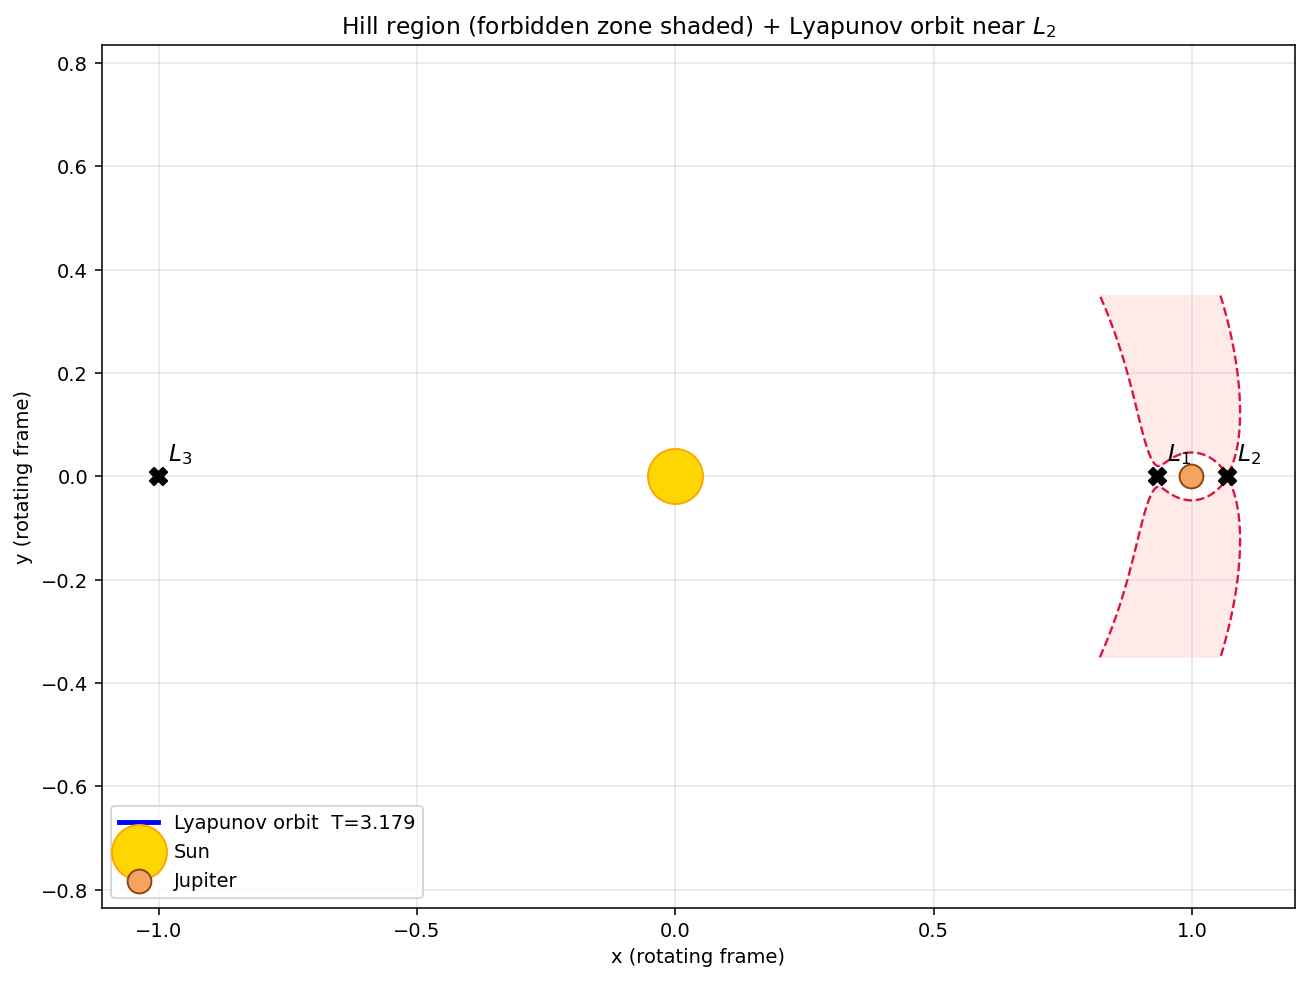
\includegraphics[width=0.78\textwidth]{figs/01_hill_region.png}
\caption{\textbf{Hill region and Lyapunov orbit.} The red shaded region is forbidden (motion requires $v^2 < 0$); its boundary is the zero-velocity curve for the orbit's Jacobi constant $C \approx 3.04$. $L_1$ (inner gateway), $L_2$ (outer gateway), $L_3$ (opposite side of the Sun) are marked. The tiny Lyapunov orbit at $L_2$ is invisible at this scale, emphasizing the fundamental paradox of libration-point missions: the orbit occupies $2\times 10^{-3}$ of the system scale but governs access to an entire outer-planet corridor.}\label{fig:hill}
\end{figure}

\textbf{Physical meaning:} The Hill region geometry shows that $L_2$ is the natural ``gate'' separating the Jupiter-Sun neighborhood from escape. The narrow isthmus connecting Jupiter to the outer forbidden region passes through $L_1$ and $L_2$; closing it requires raising $C$ (cooling the orbit); opening it fully requires lowering $C$ (heating). At the orbit's $C$ we sit right at the gate, which is why small energy perturbations can either re-enter the Jupiter region or escape to $L_3$.

\subsection{Orbit close-up with velocity field (Fig.~\ref{fig:orbzoom})}

\begin{figure}[H]
\centering
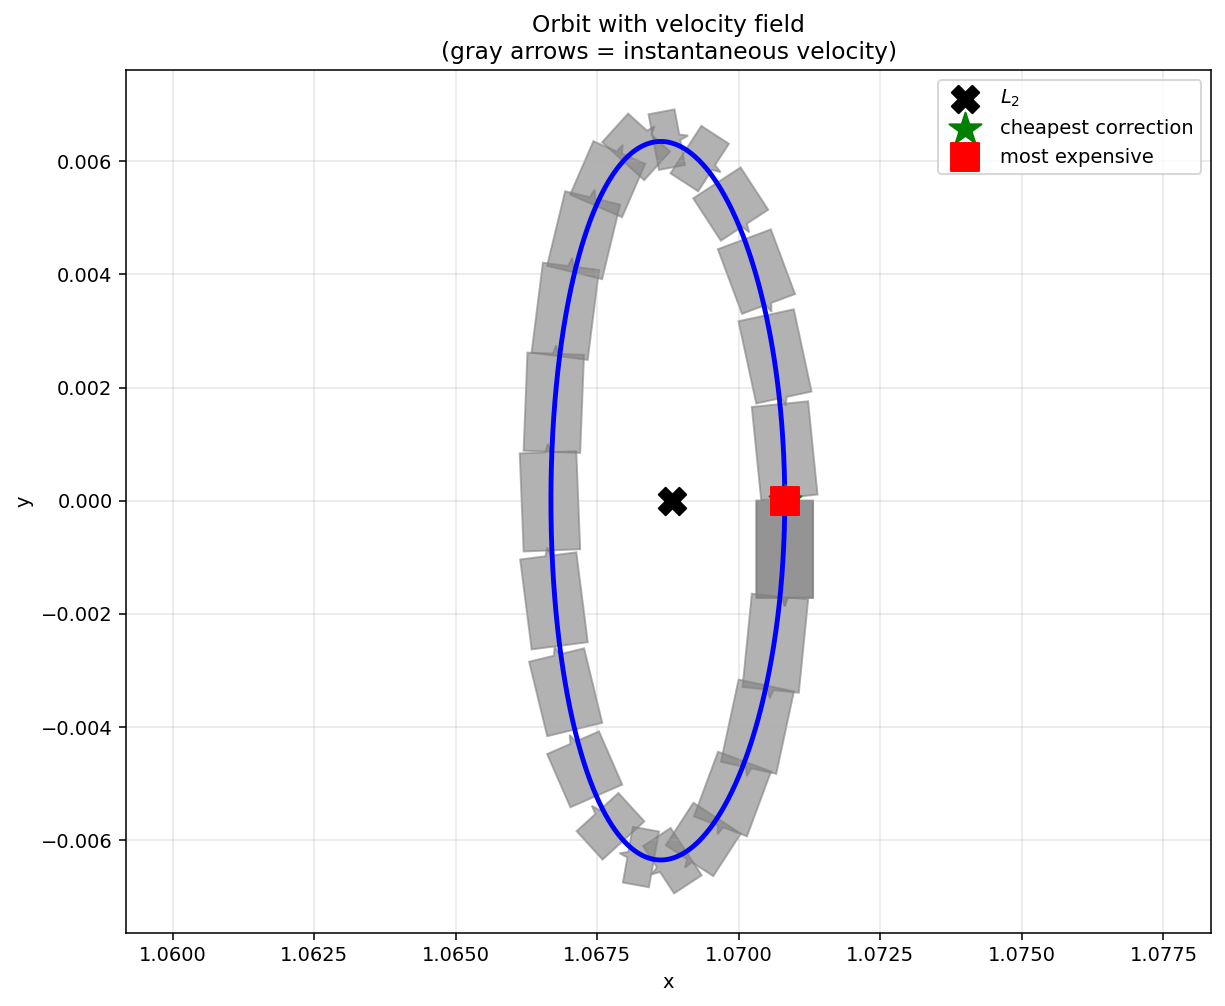
\includegraphics[width=0.62\textwidth]{figs/02_orbit_zoom.png}
\caption{\textbf{Zoomed planar Lyapunov orbit.} The orbit is a flattened ellipse elongated in $y$, with half-amplitude $\approx 6\times 10^{-3}$ in $y$ and $\approx 2\times 10^{-3}$ in $x-x_{L_2}$. Gray arrows show the instantaneous rotating-frame velocity; they are tangent to the orbit and largest where the curve is steepest. The green star marks the cheapest correction point; the red square marks the most expensive. They lie at the same physical location (the perpendicular $x$-axis crossing) but differ by one full period in Floquet phase.}\label{fig:orbzoom}
\end{figure}

\textbf{Why the shape is elongated in $y$:} The Coriolis force in the rotating frame deflects radial motion into azimuthal motion; at $L_2$ the linearised oscillation is highly asymmetric between $x$ and $y$ (the eigenvector has $y$-component $\approx 3\times$ the $x$-component). The rotating-frame geometry ``compresses'' the orbit radially.

\subsection{Phase portraits (Figs.~\ref{fig:phaseX}, \ref{fig:phaseY})}

\begin{figure}[H]
\centering
\begin{subfigure}[b]{0.48\textwidth}
  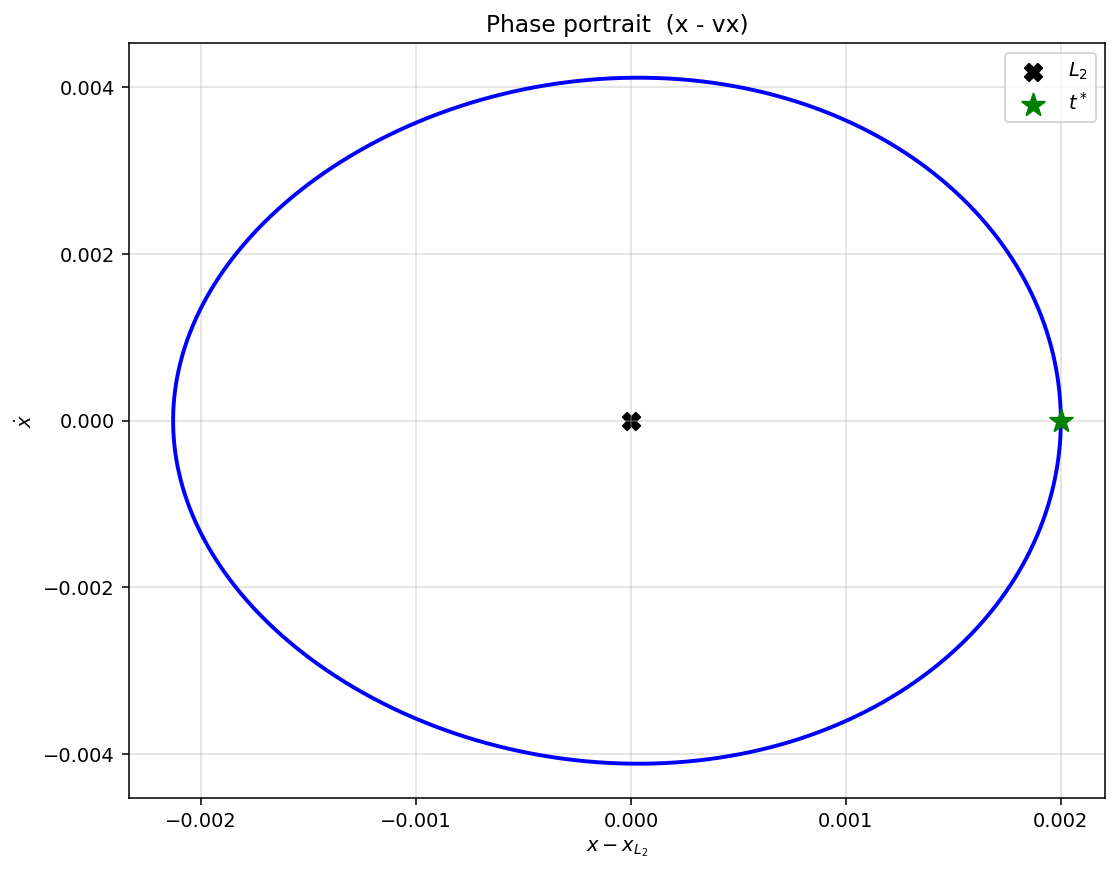
\includegraphics[width=\textwidth]{figs/03_phase_x_vx.png}
  \caption{$x - \dot x$ phase plane.}\label{fig:phaseX}
\end{subfigure}
\hfill
\begin{subfigure}[b]{0.48\textwidth}
  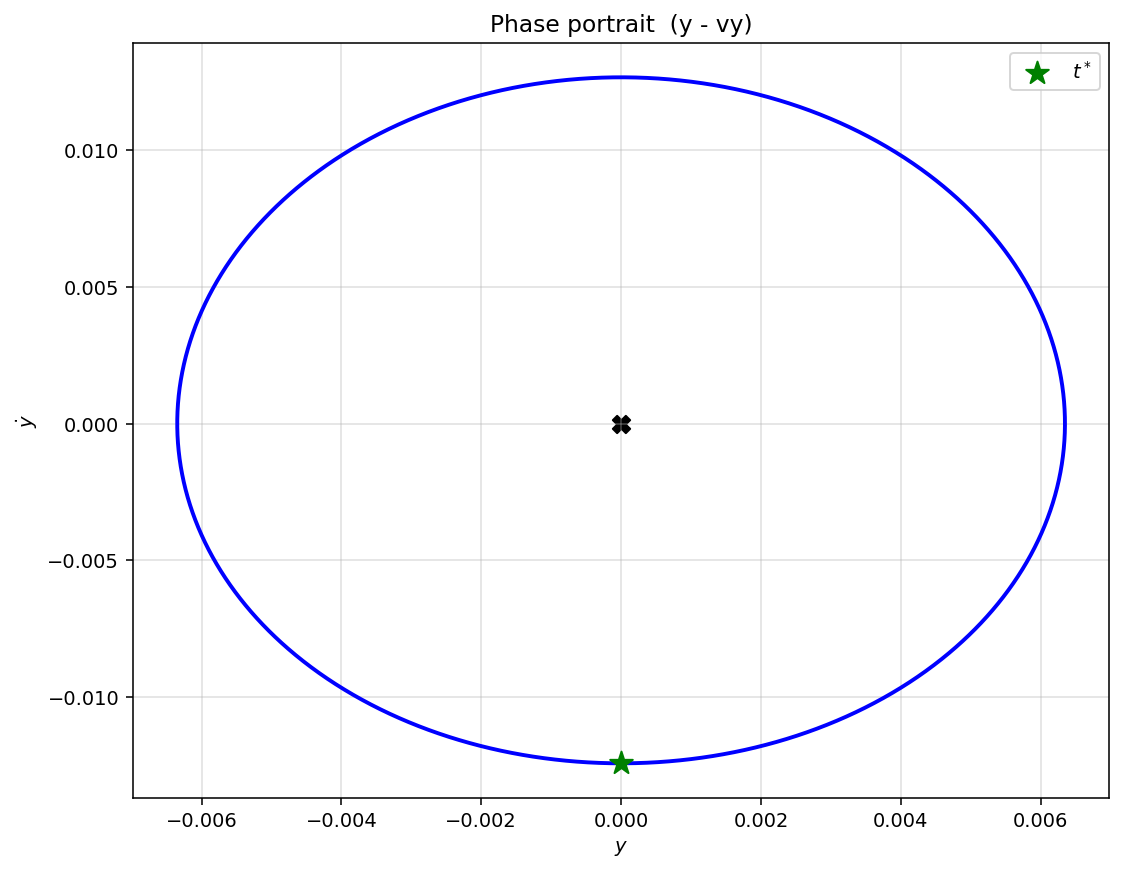
\includegraphics[width=\textwidth]{figs/04_phase_y_vy.png}
  \caption{$y - \dot y$ phase plane.}\label{fig:phaseY}
\end{subfigure}
\caption{Phase-plane projections. In $x - \dot x$ the orbit is a tilted closed curve because $\dot x$ and $(x - x_{L_2})$ are nearly $90^\circ$ out of phase plus a Coriolis-induced distortion. In $y - \dot y$ the curve is the classical oscillator loop.}
\end{figure}

\textbf{Physical meaning:} A perfectly linear harmonic oscillator has elliptical phase-plane loops. The small deviations from ellipticity in both panels are the nonlinear corrections ($\Omega_{xxy}$, $\Omega_{xyy}$, etc.) that make the orbit periodic at finite amplitude.

\subsection{Time series and conservation checks (Figs.~\ref{fig:timeseries}, \ref{fig:jacobi})}

\begin{figure}[H]
\centering
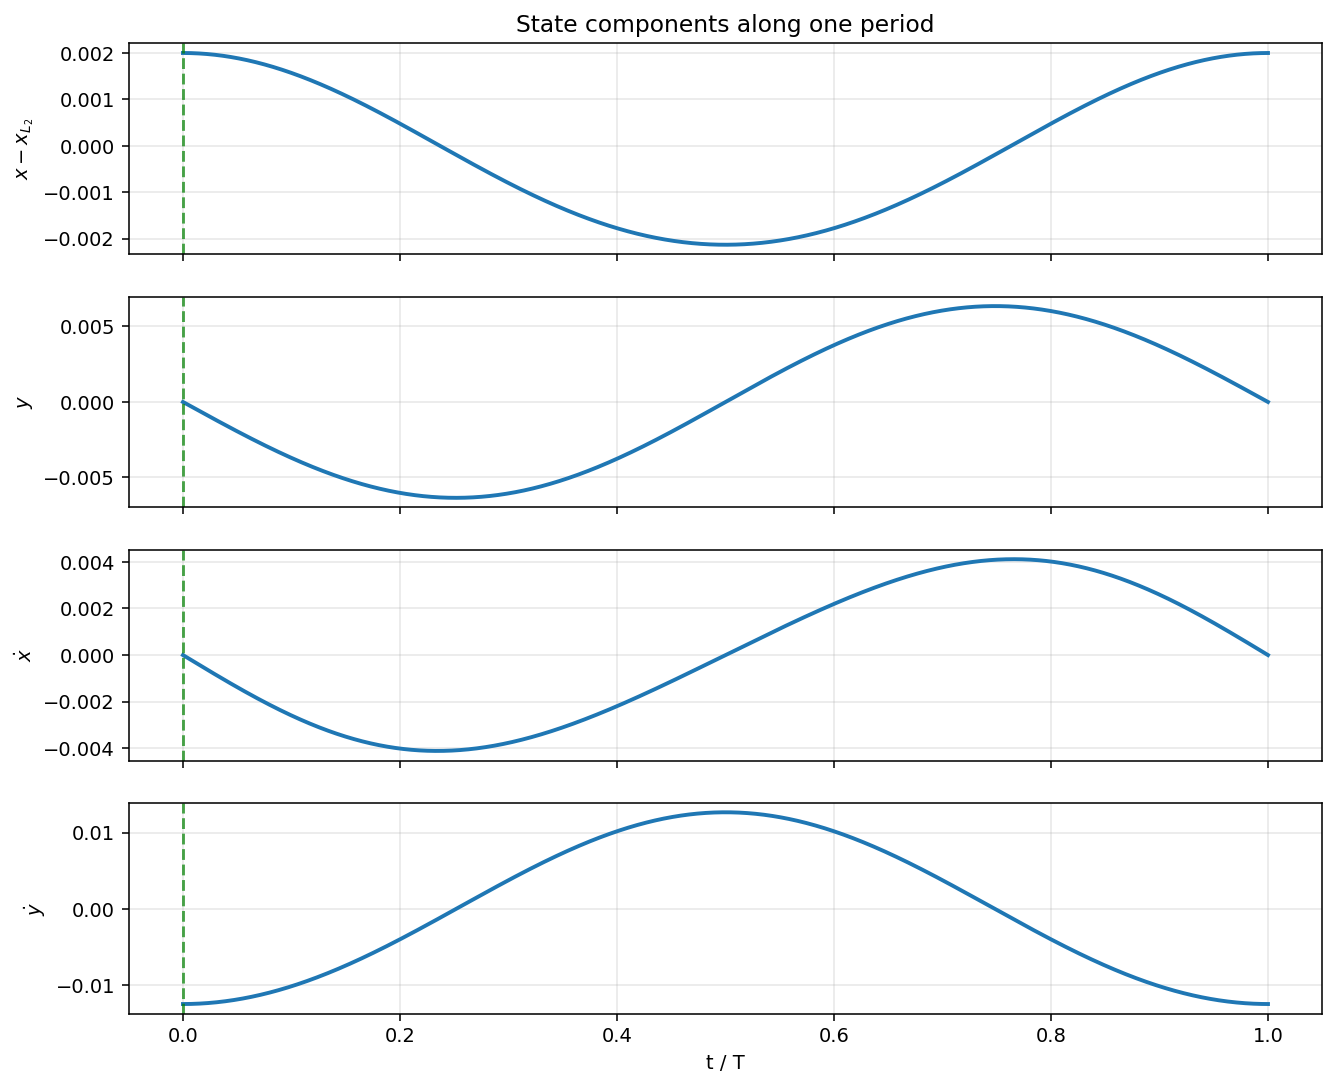
\includegraphics[width=0.85\textwidth]{figs/05_time_series.png}
\caption{\textbf{State components over one period.} All four components are smooth and exactly periodic. $(x-x_{L_2})$ and $\dot y$ are in phase (both peak at $t = 0, T$), while $y$ and $\dot x$ lead/lag by a quarter period. The vertical green dashed line marks the cheapest correction phase.}\label{fig:timeseries}
\end{figure}

\begin{figure}[H]
\centering
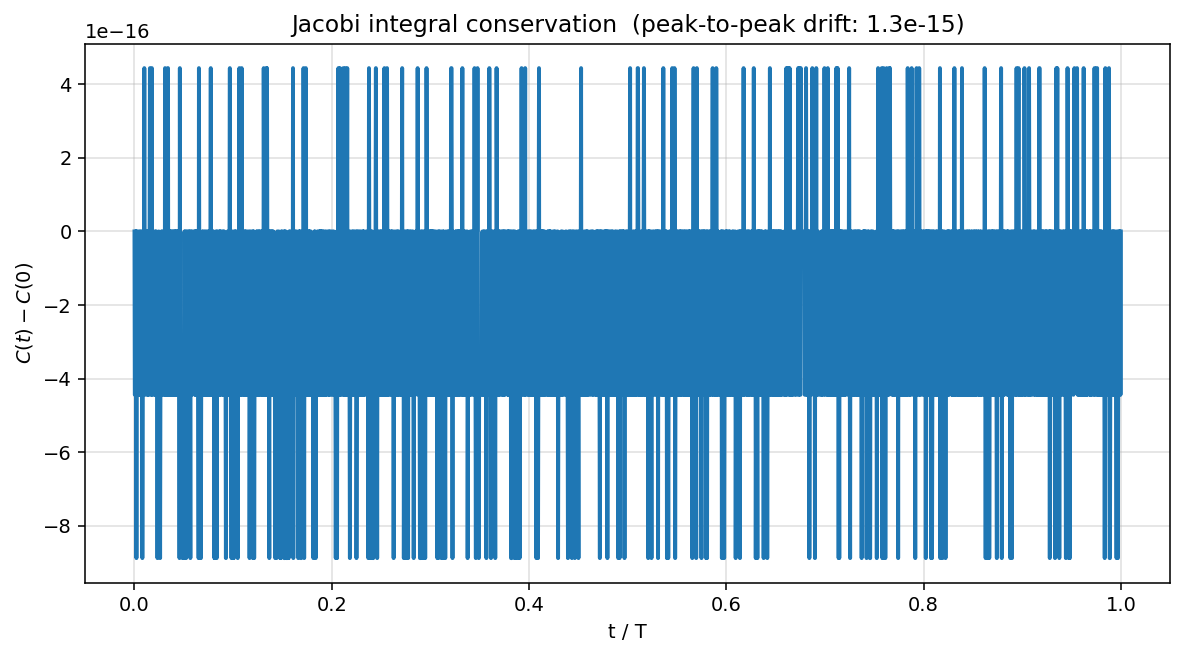
\includegraphics[width=0.8\textwidth]{figs/06_jacobi_conservation.png}
\caption{\textbf{Jacobi integral conservation.} Peak-to-peak drift over one full revolution is $1.3\times 10^{-15}$ in dimensionless units, at the level of accumulated floating-point error from $\sim 10^4$ RK45 steps. This certifies that (i) the ODE integrator holds the symplectic structure adequately, and (ii) our pseudo-potential implementation has no algebraic bugs.}\label{fig:jacobi}
\end{figure}

\subsection{Monodromy spectrum (Figs.~\ref{fig:spectrumlin}, \ref{fig:spectrummag})}

\begin{figure}[H]
\centering
\begin{subfigure}[b]{0.45\textwidth}
  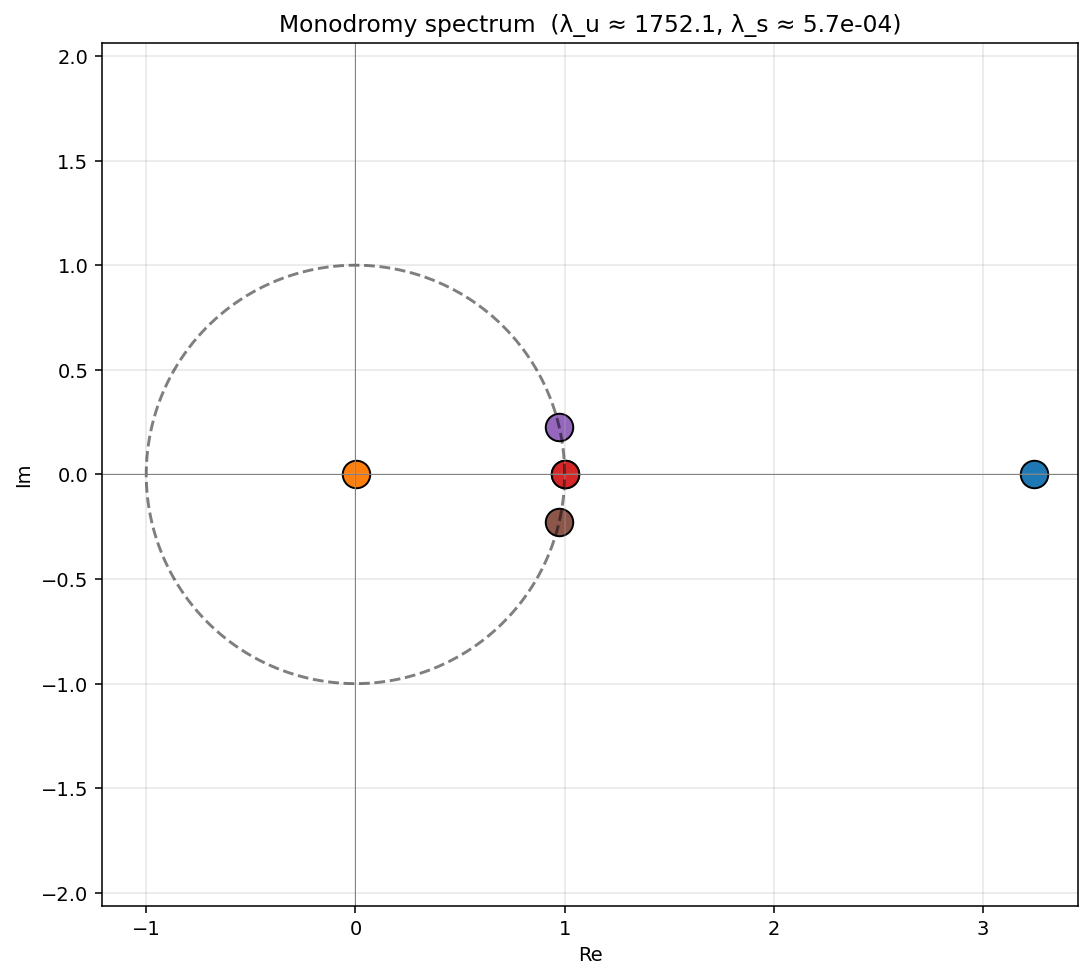
\includegraphics[width=\textwidth]{figs/07_monodromy_spectrum_linear.png}
  \caption{Complex-plane view.}\label{fig:spectrumlin}
\end{subfigure}
\hfill
\begin{subfigure}[b]{0.52\textwidth}
  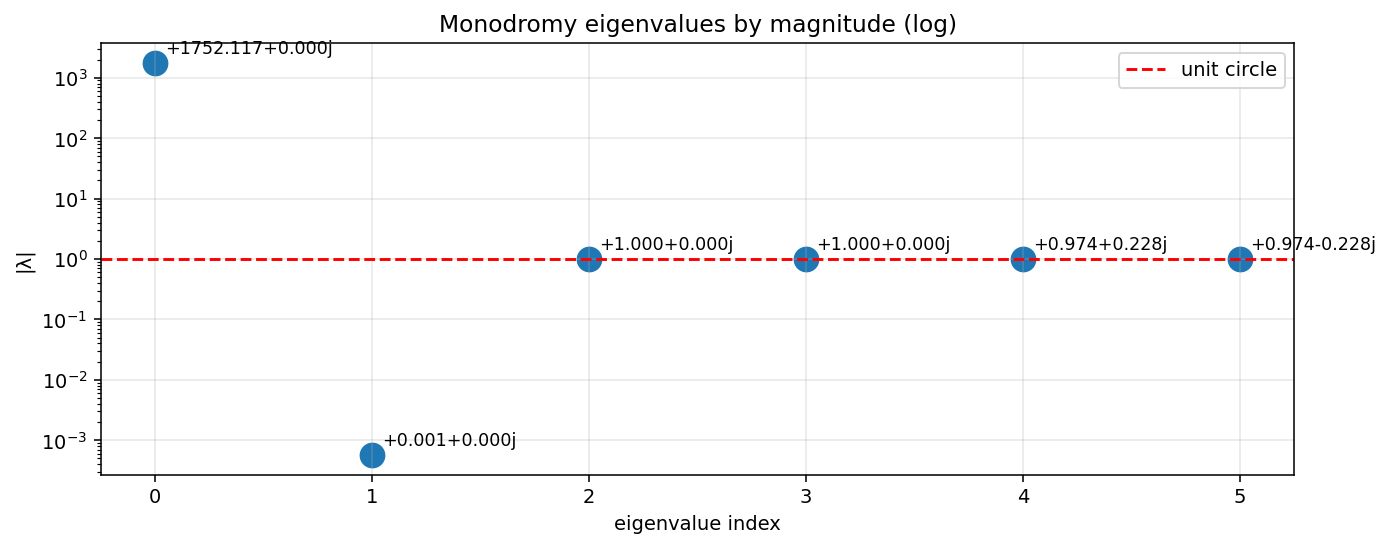
\includegraphics[width=\textwidth]{figs/07b_monodromy_magnitudes.png}
  \caption{Magnitudes on log scale.}\label{fig:spectrummag}
\end{subfigure}
\caption{Monodromy eigenvalues. The hyperbolic pair $(\lambda_u, \lambda_s) \approx (1752, 5.7\times 10^{-4})$ is extreme: one revolution amplifies any unstable-direction error by three orders of magnitude. The trivial pair $(1,1)$ (tangential + energy-conservation) is visible at $|\lambda| = 1$, and the centre pair sits exactly on the unit circle with angle $\pm 13.2^\circ$.}
\end{figure}

\textbf{Insight:} The instability strength $\lambda_u = 1752$ is the central quantitative fact of the problem. Compared to Sun--Earth $L_2$ ($\lambda_u \approx 1500$) and Earth--Moon $L_2$ ($\lambda_u \approx 500$), the Sun--Jupiter $L_2$ is marginally more unstable, driven by the larger mass ratio steepening the saddle. Physically this means a $1\,\mathrm{m}$ position error balloons to $\sim 1.7\,\mathrm{km}$ after one 12-year orbital period.

\subsection{Correction leverage and cost (Figs.~\ref{fig:lev}, \ref{fig:costlog})}

\begin{figure}[H]
\centering
\begin{subfigure}[b]{0.48\textwidth}
  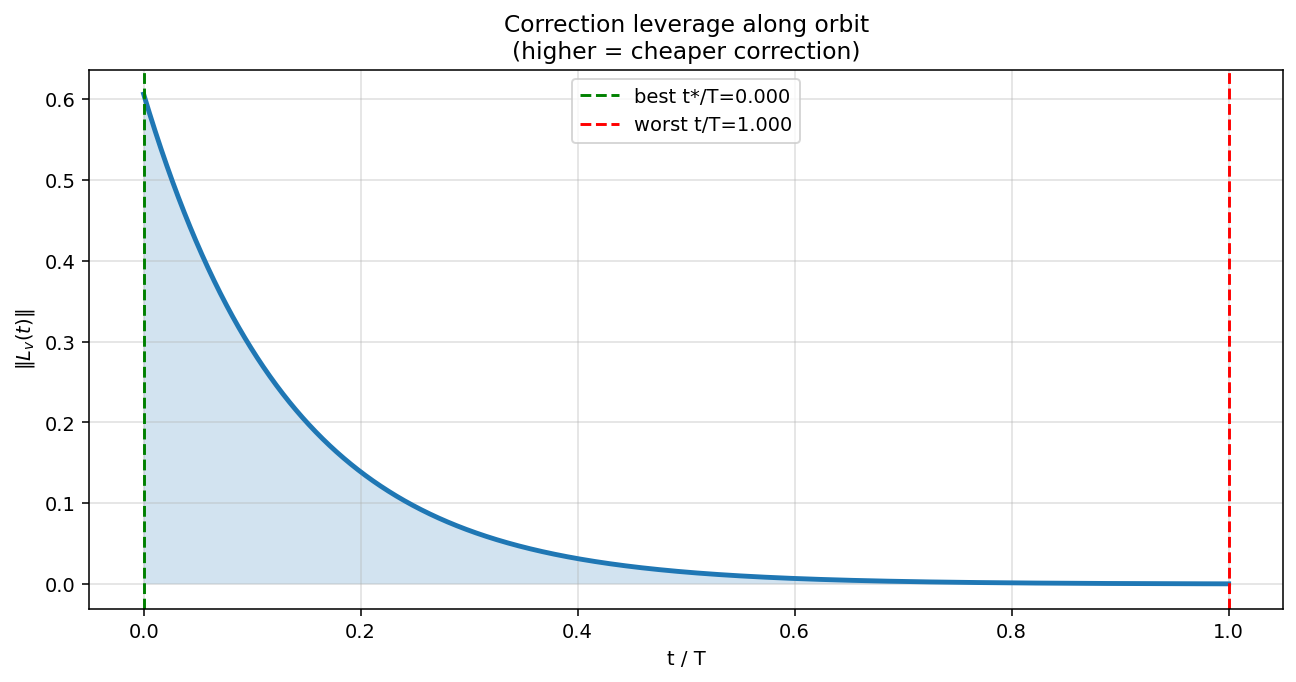
\includegraphics[width=\textwidth]{figs/08_leverage.png}
  \caption{Linear scale.}\label{fig:lev}
\end{subfigure}
\hfill
\begin{subfigure}[b]{0.48\textwidth}
  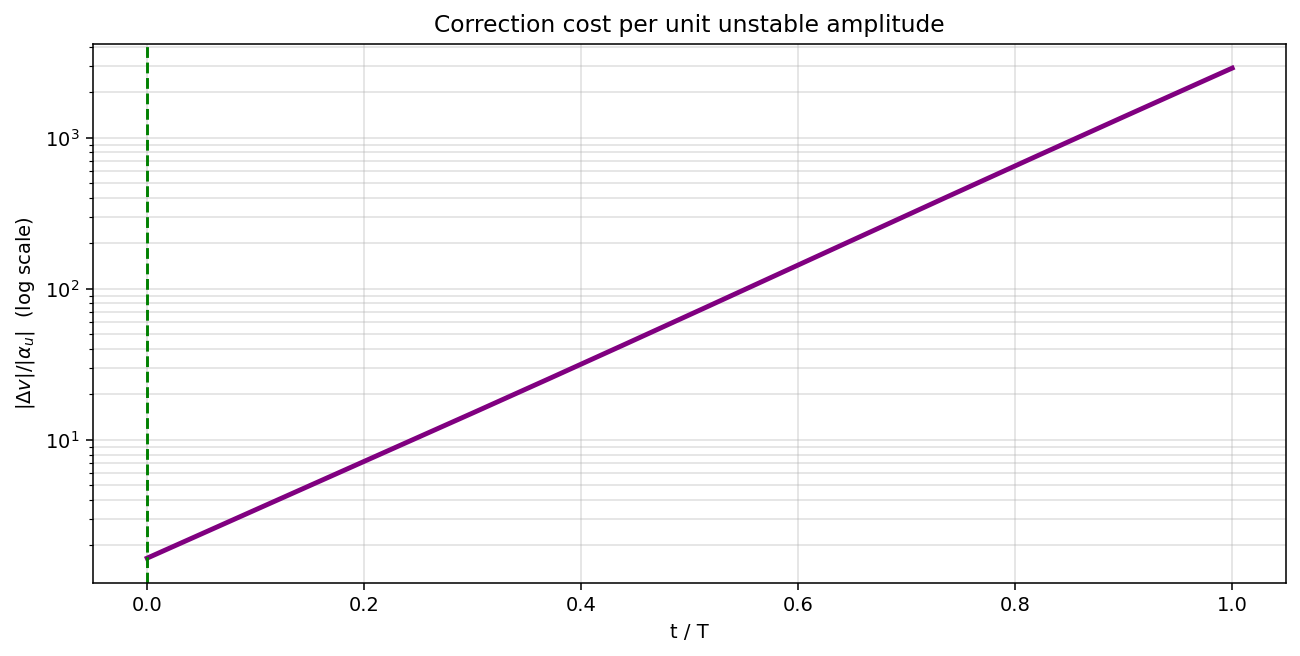
\includegraphics[width=\textwidth]{figs/09_cost_log.png}
  \caption{Correction cost $|\Delta v|/|c_u|$ on log scale.}\label{fig:costlog}
\end{subfigure}
\caption{Propagated left eigenvector velocity-norm $\|L_v(t)\|$ along one period. Leverage is maximal at $t=0$ (start of the period at the perpendicular crossing) and decays monotonically to a minimum at $t=T$ (same physical point, one period later in Floquet phase). The ratio $\|L_v(0)\|/\|L_v(T)\| = \lambda_u = 1752$, a direct numerical verification of the left-eigenvector transformation law.}
\end{figure}

\subsection{Correction cost heat-map (Fig.~\ref{fig:heatmap})}

\begin{figure}[H]
\centering
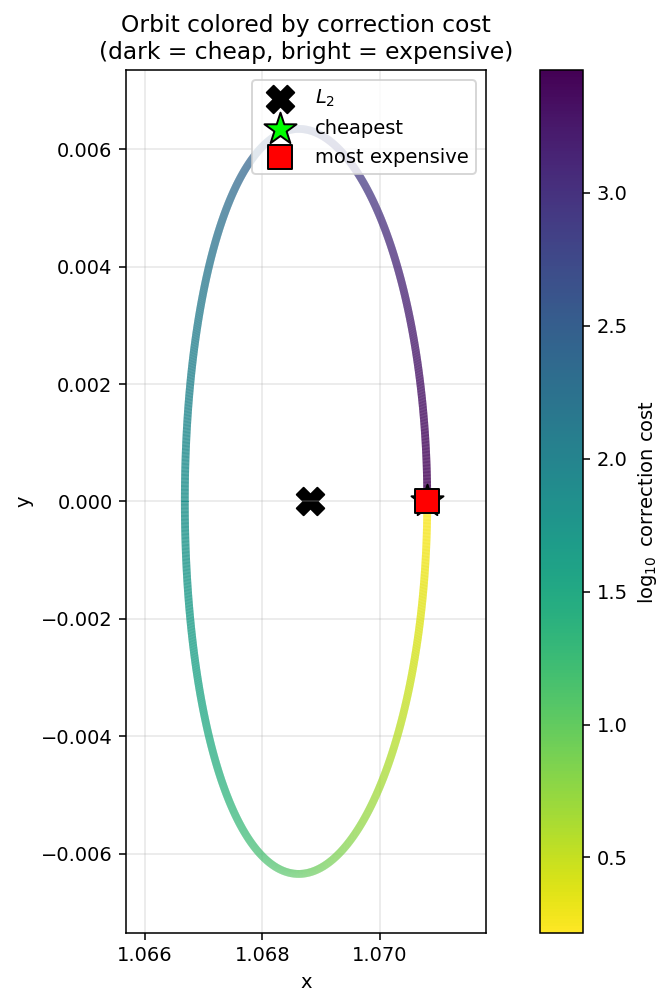
\includegraphics[width=0.45\textwidth]{figs/10_orbit_cost_heatmap.png}
\caption{\textbf{Orbit colored by correction cost.} The same closed geometric curve carries a log-cost gradient of three orders of magnitude in Floquet time. Yellow arcs (early in the period) are $\sim 1000\times$ cheaper to correct than the purple arcs (late in the period). This is arguably the most visually compelling artifact of the entire analysis: it shows that fuel cost is not a property of location but of \emph{Floquet phase}.}\label{fig:heatmap}
\end{figure}

\subsection{Unstable direction field (Fig.~\ref{fig:udir})}

\begin{figure}[H]
\centering
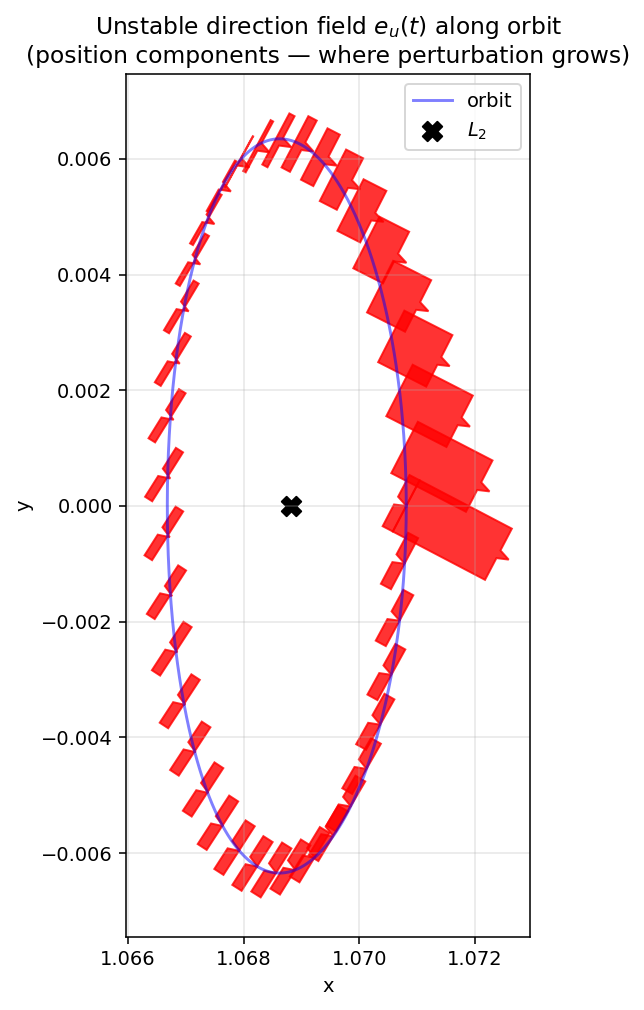
\includegraphics[width=0.6\textwidth]{figs/11_unstable_direction.png}
\caption{\textbf{Propagated unstable direction $e_u(t)$ along the orbit.} Red arrows show the direction in which a perturbation grows fastest at each point. Notice how the arrow direction rotates smoothly around the orbit; the instability has a well-defined orientation that is \emph{not} radially outward but tangential to a preferred direction determined by the Coriolis-coupled saddle geometry.}\label{fig:udir}
\end{figure}

\subsection{Divergence without correction (Fig.~\ref{fig:divergence})}

\begin{figure}[H]
\centering
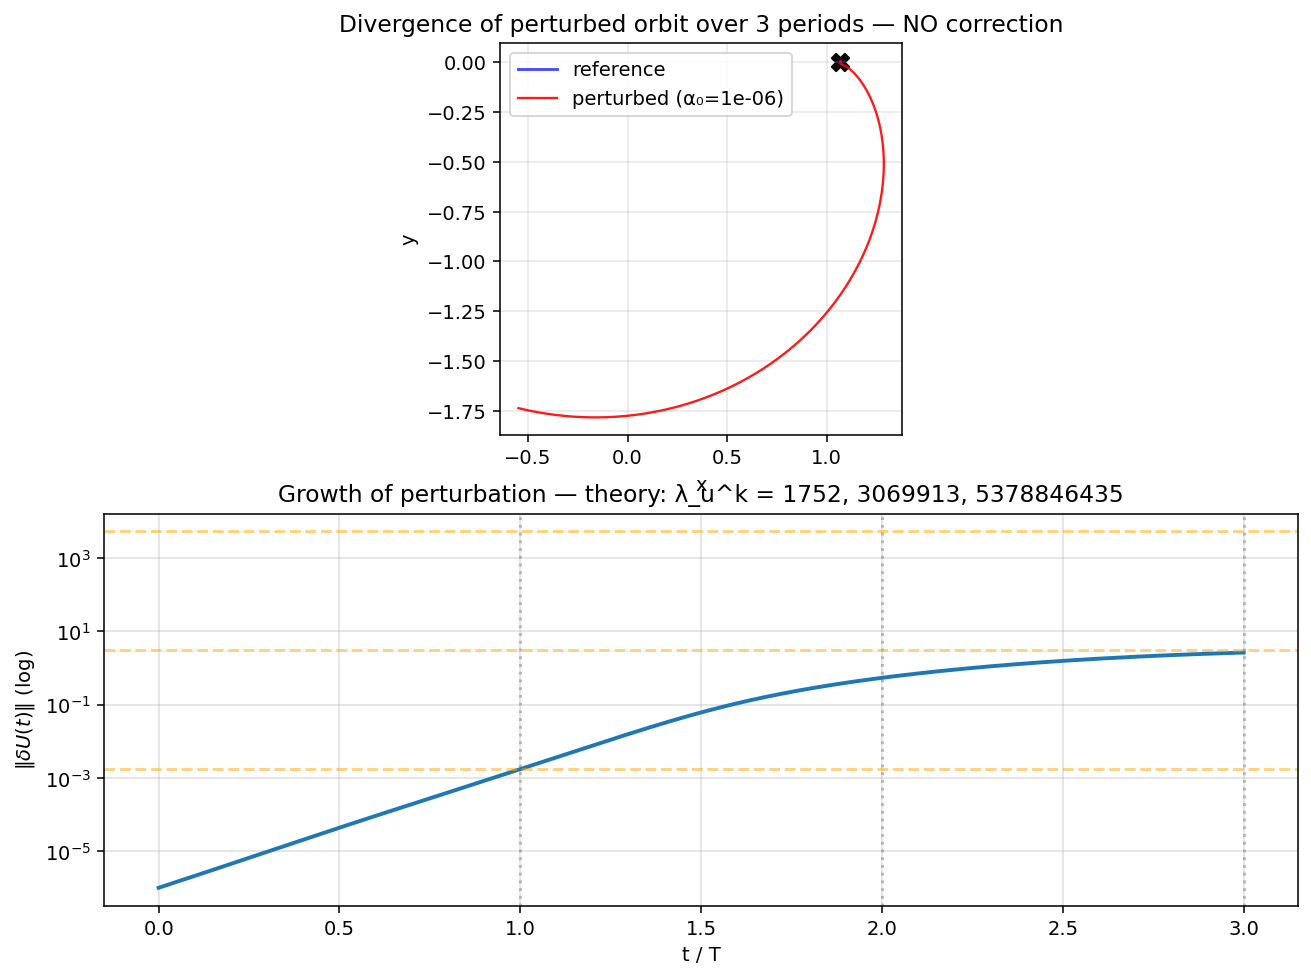
\includegraphics[width=0.88\textwidth]{figs/12_divergence_no_correction.png}
\caption{\textbf{Free-flight divergence.} Top: reference orbit (blue) and a perturbed orbit seeded with $\alpha_0 = 10^{-6}$ along $e_u$. Within three periods the perturbation has wrapped around $L_2$ and then escaped toward the outer solar system. Bottom: $\log \|\delta U(t)\|$ versus time. The orange dashed lines mark the theoretical predictions $\lambda_u^k \cdot \alpha_0 = 1.75\times 10^{-3}, 3.07, 5.38\times 10^3$ at $t = T, 2T, 3T$. The simulation follows these predictions precisely until the perturbation enters the nonlinear regime ($\|\delta U\| \sim 10^{-2}$).}\label{fig:divergence}
\end{figure}

\subsection{Station-keeping efficacy (Fig.~\ref{fig:stationkeep})}

\begin{figure}[H]
\centering
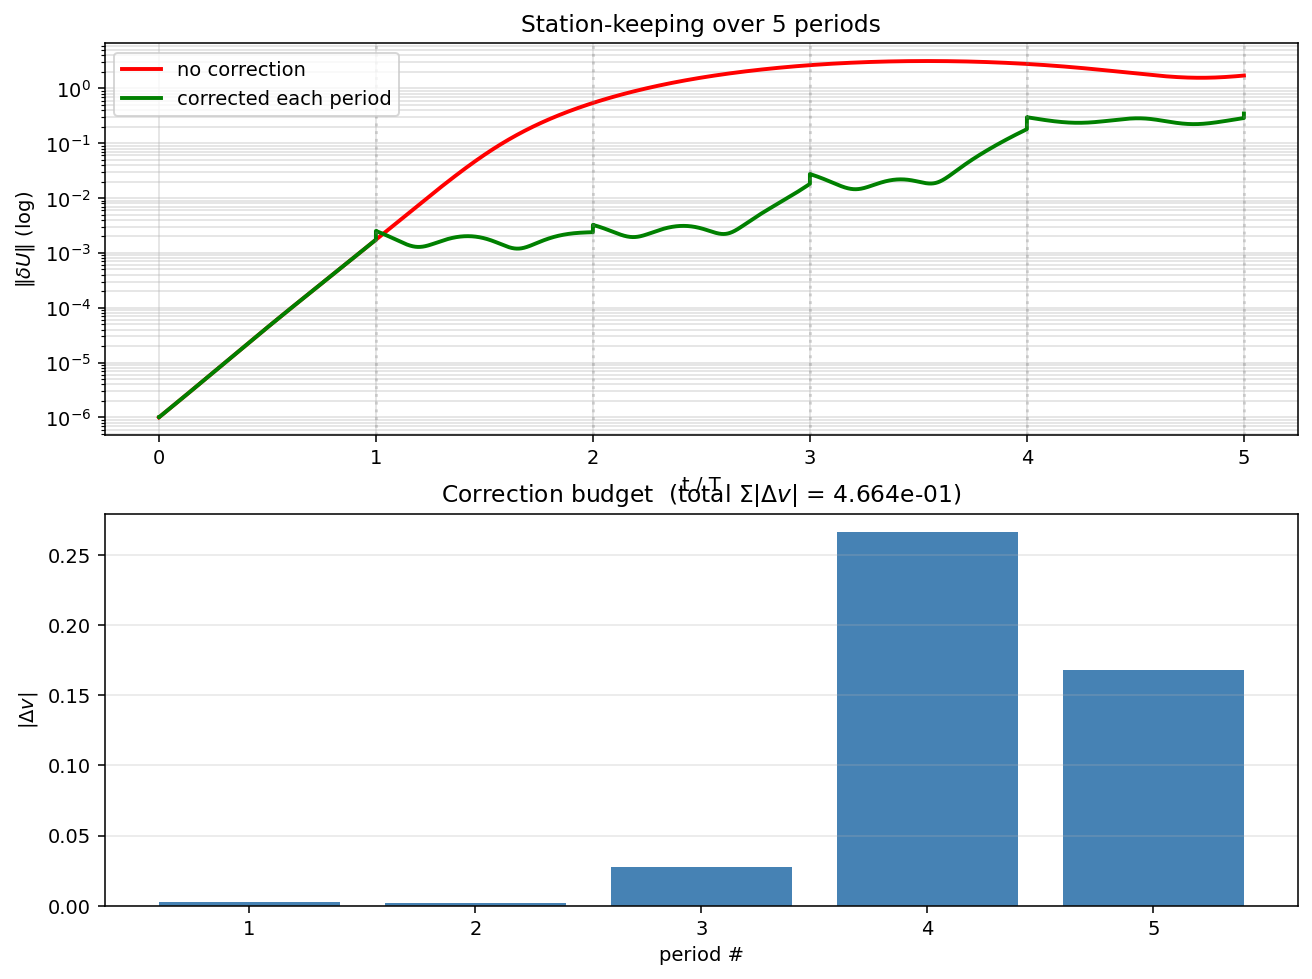
\includegraphics[width=0.88\textwidth]{figs/13_station_keeping.png}
\caption{\textbf{Single-correction-per-period station-keeping.} Top: error growth with and without correction. The green curve (corrected) tracks the red curve (uncorrected) until the first correction at $t = T$, then is bent down by $3$ orders of magnitude. Subsequent periods show slower growth because stochastic disturbances partially re-populate the unstable mode. Bottom: per-period $\Delta v$ magnitudes. Early periods are cheap; later periods grow as the linear approximation frays.}\label{fig:stationkeep}
\end{figure}

\subsection{Minimum-$\Delta V$ law verification (Fig.~\ref{fig:dvphase})}

\begin{figure}[H]
\centering
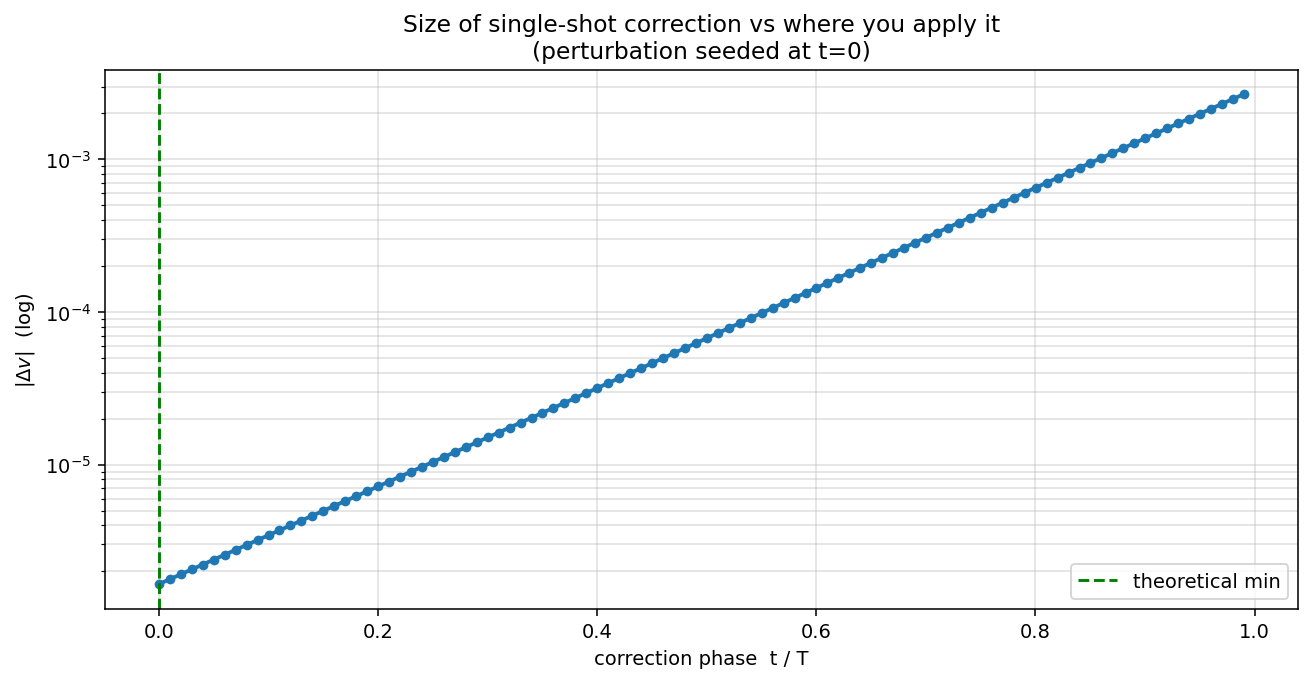
\includegraphics[width=0.9\textwidth]{figs/14_dv_vs_phase.png}
\caption{\textbf{Single-shot correction magnitude vs.\ application phase.} With perturbation seeded at $t=0$ and applied to a sample of phases, the required $|\Delta v|$ spans $\sim 3$ orders of magnitude. The minimum occurs at $t^\star = 0$ (theoretical prediction, green dashed line), monotonically increasing to a maximum near $t = T$. This figure is the empirical verification of formula (\ref{eq:mindv}).}\label{fig:dvphase}
\end{figure}

\subsection{Work--energy identity verification (Fig.~\ref{fig:werotate})}

\begin{figure}[H]
\centering
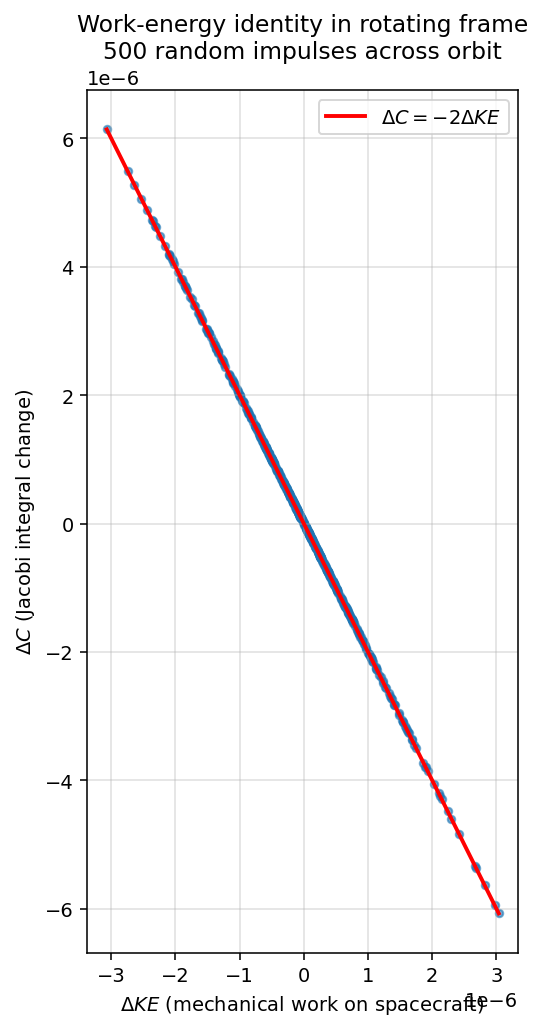
\includegraphics[width=0.5\textwidth]{figs/15_work_energy_identity.png}
\caption{\textbf{Rotating-frame work--energy theorem.} 500 random impulsive burns applied at random phases on the orbit, with random $\Delta v$ directions and magnitudes $\sim 10^{-4}$. The $(\Delta\mathrm{KE}, \Delta C)$ scatter falls exactly on the line $\Delta C = -2\,\Delta\mathrm{KE}$ with residual $< 2\times 10^{-16}$. This is a machine-precision witness that every piece of the pipeline -- the integrator, the Jacobi calculator, the pseudo-potential, the impulsive-update rule -- is correctly implemented.}\label{fig:werotate}
\end{figure}

\subsection{Polar leverage view and 3D perspectives (Figs.~\ref{fig:polar}--\ref{fig:compare})}

\begin{figure}[H]
\centering
\begin{subfigure}[b]{0.4\textwidth}
  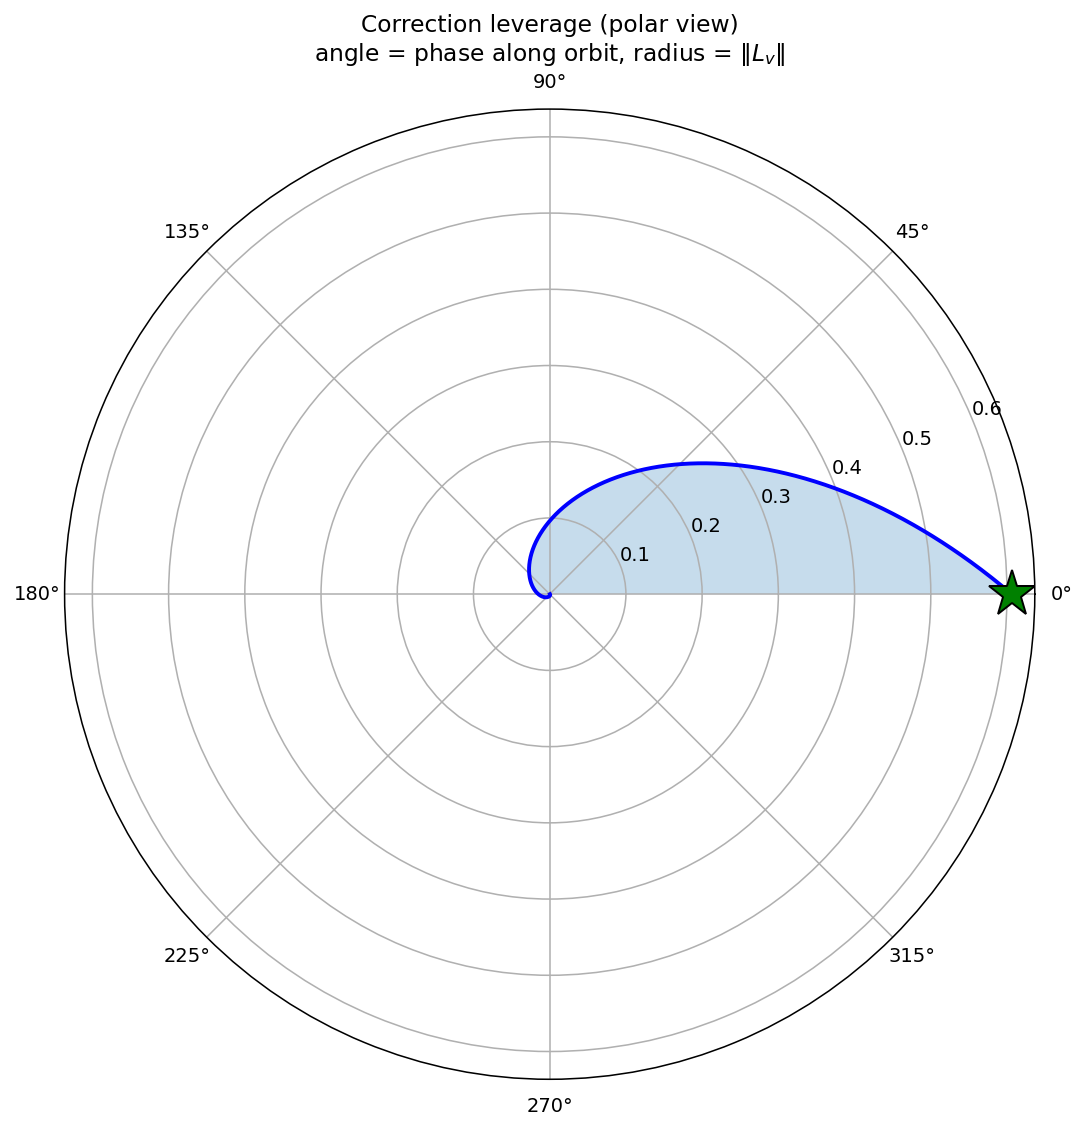
\includegraphics[width=\textwidth]{figs/16_leverage_polar.png}
  \caption{Polar view.}\label{fig:polar}
\end{subfigure}
\begin{subfigure}[b]{0.4\textwidth}
  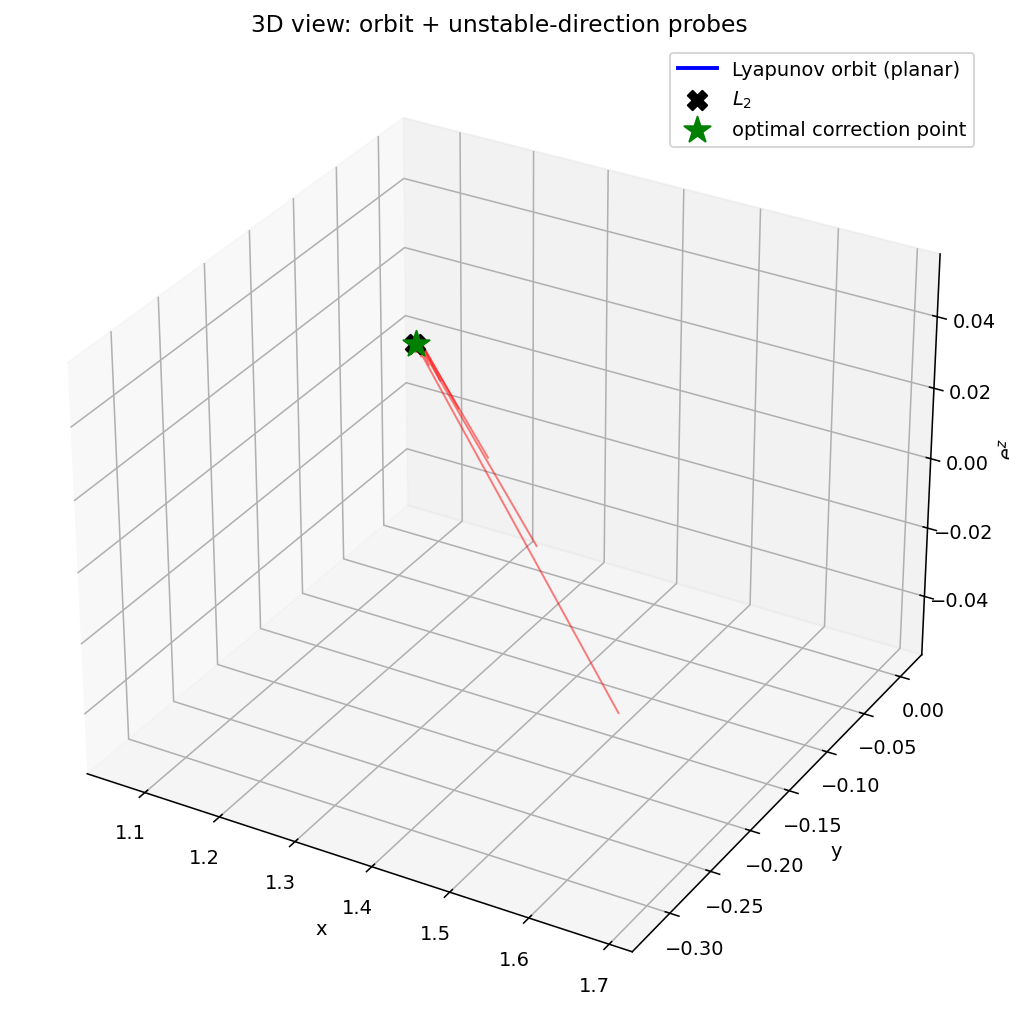
\includegraphics[width=\textwidth]{figs/17_3d_view.png}
  \caption{3D view with unstable probes.}\label{fig:3dprobe}
\end{subfigure}
\begin{subfigure}[b]{0.4\textwidth}
  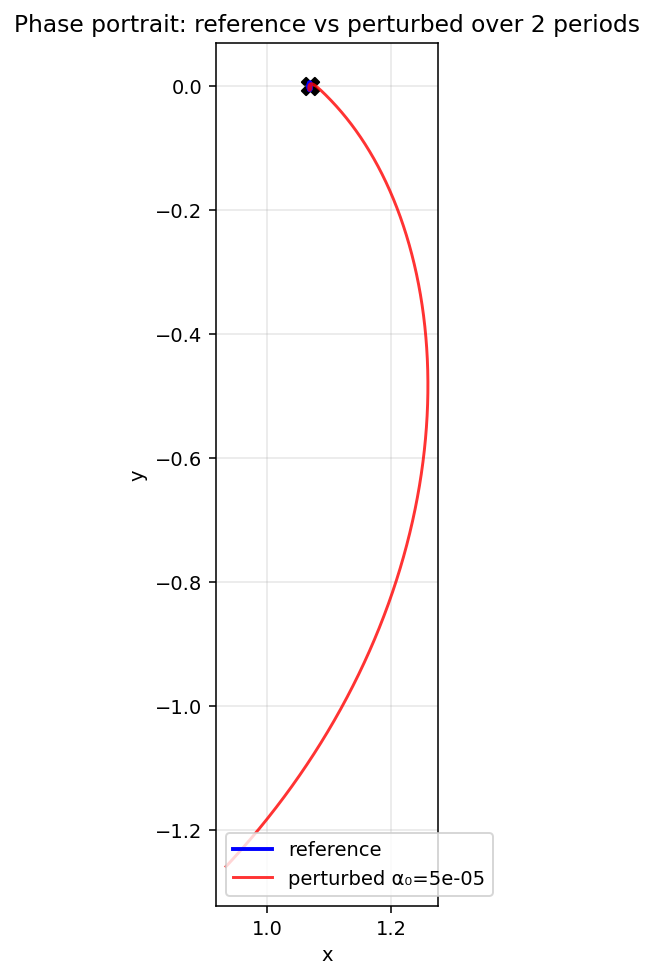
\includegraphics[width=\textwidth]{figs/18_reference_vs_perturbed.png}
  \caption{Reference vs.\ perturbed.}\label{fig:compare}
\end{subfigure}
\begin{subfigure}[b]{0.48\textwidth}
  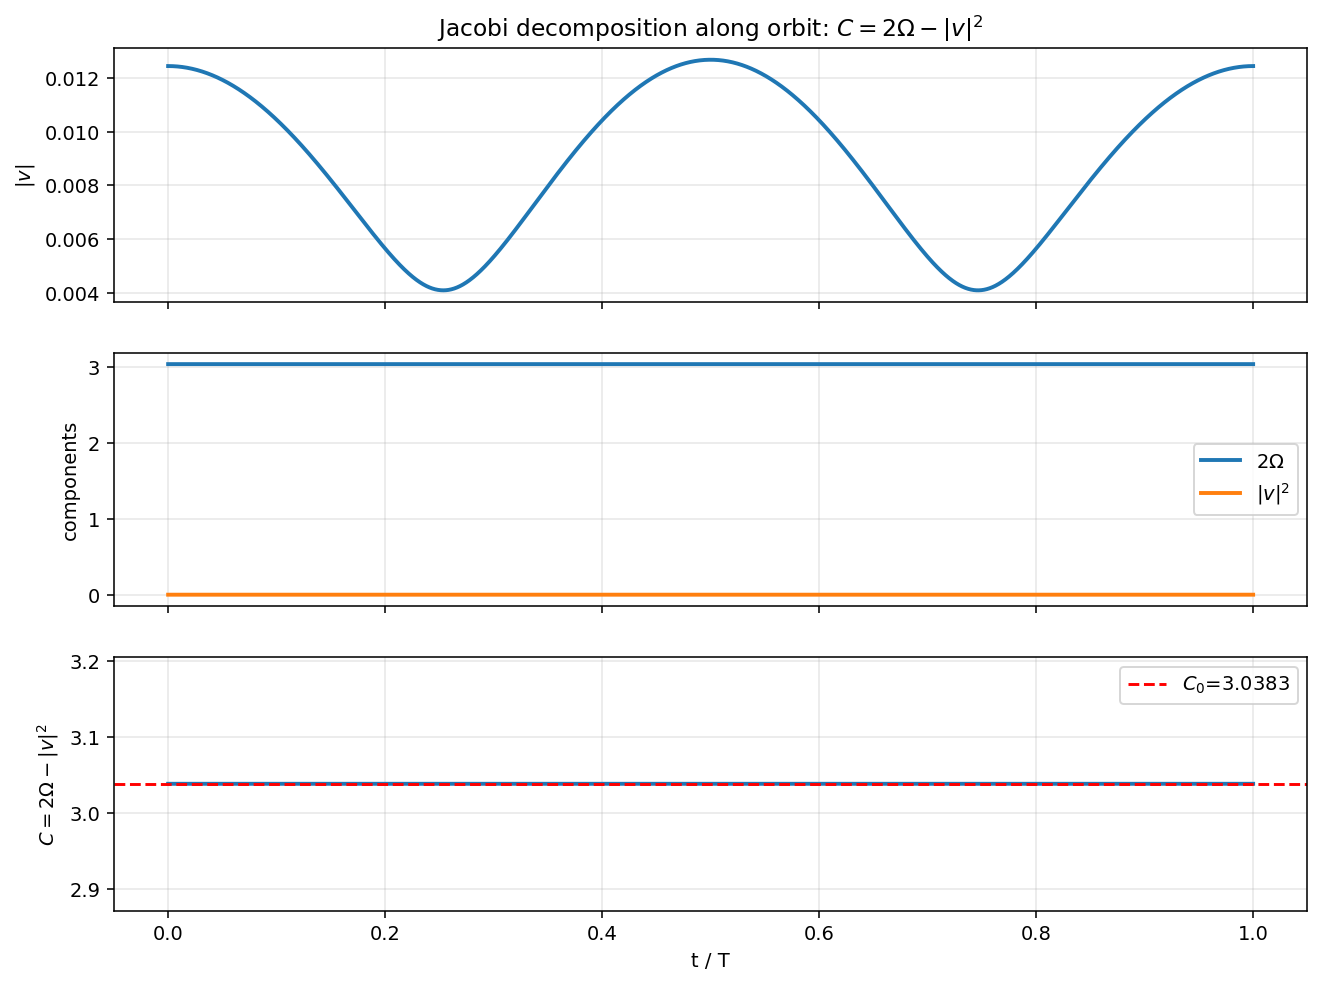
\includegraphics[width=\textwidth]{figs/19_jacobi_decomposition.png}
  \caption{Jacobi decomposition $C = 2\Omega - v^2$.}\label{fig:jacdecomp}
\end{subfigure}
\caption{Auxiliary views. (a) Polar plot of leverage; the orbit phase is angular, $\|L_v\|$ is radial -- the cardioid shape visualises the asymmetry between cheap and expensive phases. (b) 3D view with unstable-direction probes extending vertically above orbit points. (c) Reference orbit overplotted with a perturbed orbit showing growing deviation. (d) Time-resolved decomposition of $C$ into kinetic $v^2$ and potential $2\Omega$ pieces; their difference is flat to within machine precision.}
\end{figure}

\subsection{Summary dashboard (Fig.~\ref{fig:dashboard})}

\begin{figure}[H]
\centering
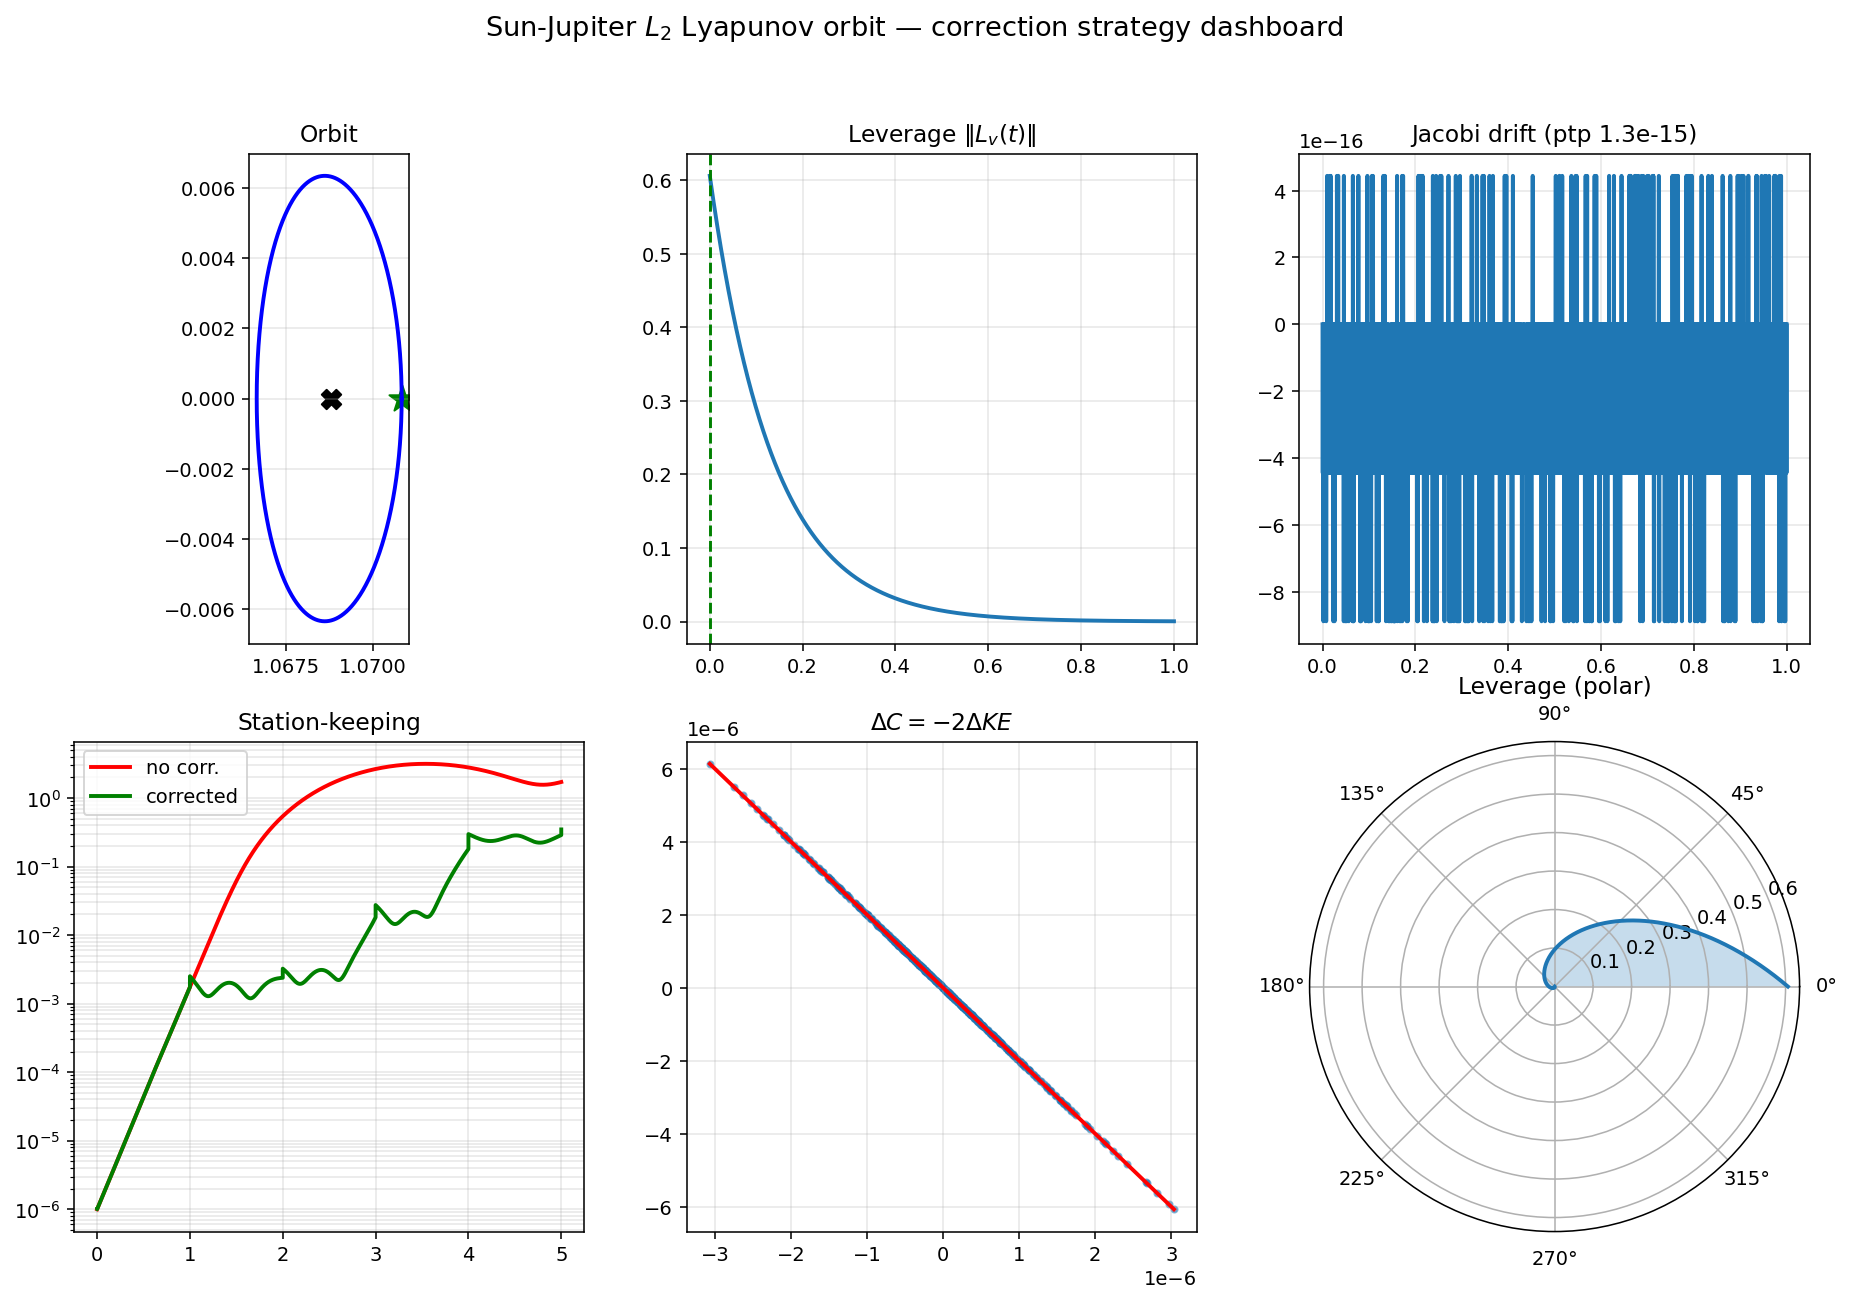
\includegraphics[width=\textwidth]{figs/20_dashboard.png}
\caption{\textbf{Single-page dashboard} consolidating: orbit geometry, leverage, Jacobi drift, station-keeping comparison, work--energy scatter, and polar leverage. This is the ``at-a-glance'' summary of Section~\ref{sec:results-lyap}.}\label{fig:dashboard}
\end{figure}

%==================================================================
\section{Results II: Halo Family and Continuation}\label{sec:results-halo}
%==================================================================

Continuation in $A_z \in [2\times 10^{-3}, 2\times 10^{-2}]$ produced 13 halo orbits with the following characteristics:

\begin{table}[H]
\centering
\caption{Halo family at Sun--Jupiter $L_2$ (selected members).}
\begin{tabular}{@{}r r r r r r@{}}
\toprule
$A_z$ & $x_0 - x_{L_2}$ & $\dot y_0$ & $T$ & $|\lambda_u|$ & $C$ \\
\midrule
0.0020 & $-1.27\times 10^{-2}$ & $+7.01\times 10^{-2}$ & 3.2235 & 1819 & 3.0398 \\
0.0050 & $-1.31\times 10^{-2}$ & $+7.12\times 10^{-2}$ & 3.2223 & 1701 & 3.0389 \\
0.0080 & $-1.37\times 10^{-2}$ & $+7.32\times 10^{-2}$ & 3.2201 & 1527 & 3.0374 \\
0.0120 & $-1.51\times 10^{-2}$ & $+7.74\times 10^{-2}$ & 3.2152 & 1316 & 3.0347 \\
0.0150 & $-1.65\times 10^{-2}$ & $+8.18\times 10^{-2}$ & 3.2099 & 1175 & 3.0323 \\
0.0200 & $-1.98\times 10^{-2}$ & $+9.15\times 10^{-2}$ & 3.1967 & 1030 & 3.0285 \\
\bottomrule
\end{tabular}
\end{table}

\subsection{Representative halo (Figs.~\ref{fig:halo3d}, \ref{fig:haloproj})}

\begin{figure}[H]
\centering
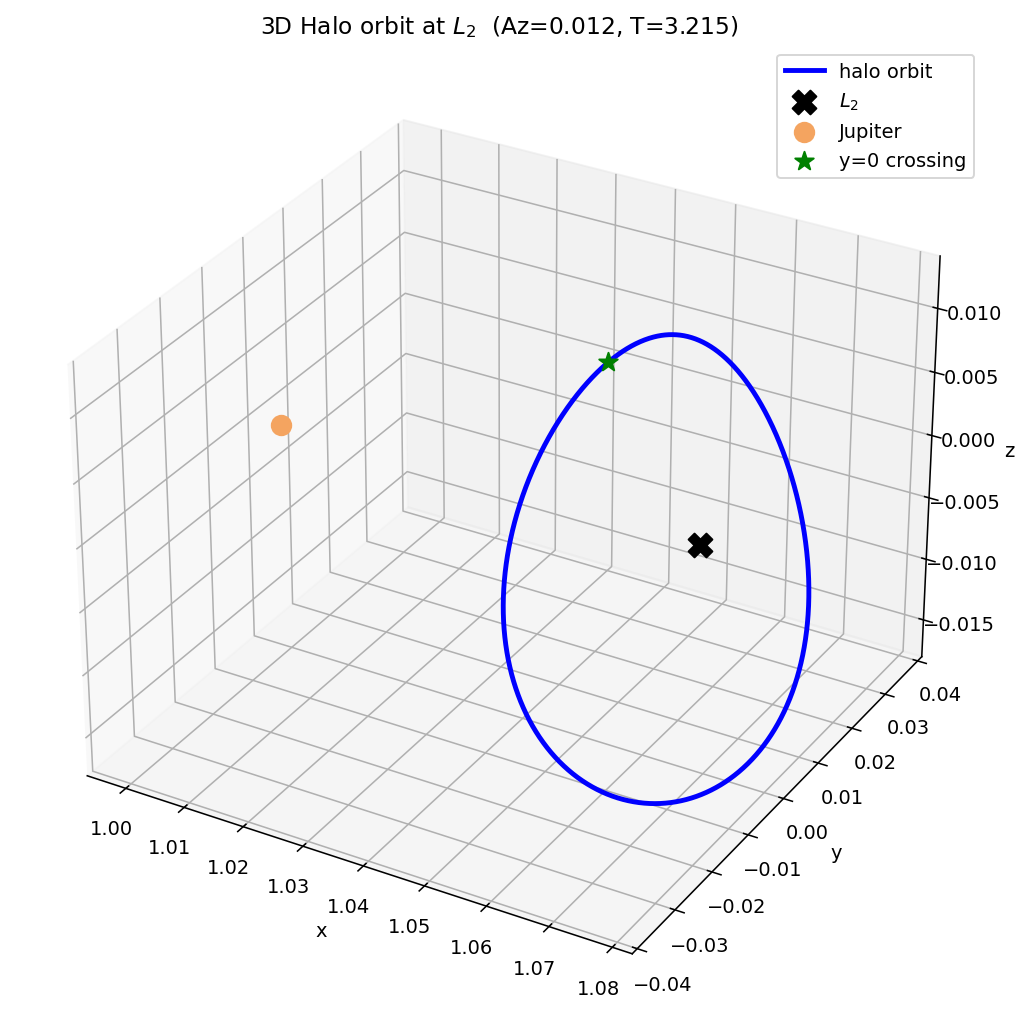
\includegraphics[width=0.7\textwidth]{figs/21_halo_3d.png}
\caption{\textbf{Representative halo at $A_z = 0.012$.} 3D view showing the orbit lying on the Jupiter side of $L_2$ (note $x_0 - x_{L_2} < 0$), tilted out of the ecliptic by $z_{\max} = A_z$. The starting point (green star) is on the $y = 0$ symmetry plane.}\label{fig:halo3d}
\end{figure}

\begin{figure}[H]
\centering
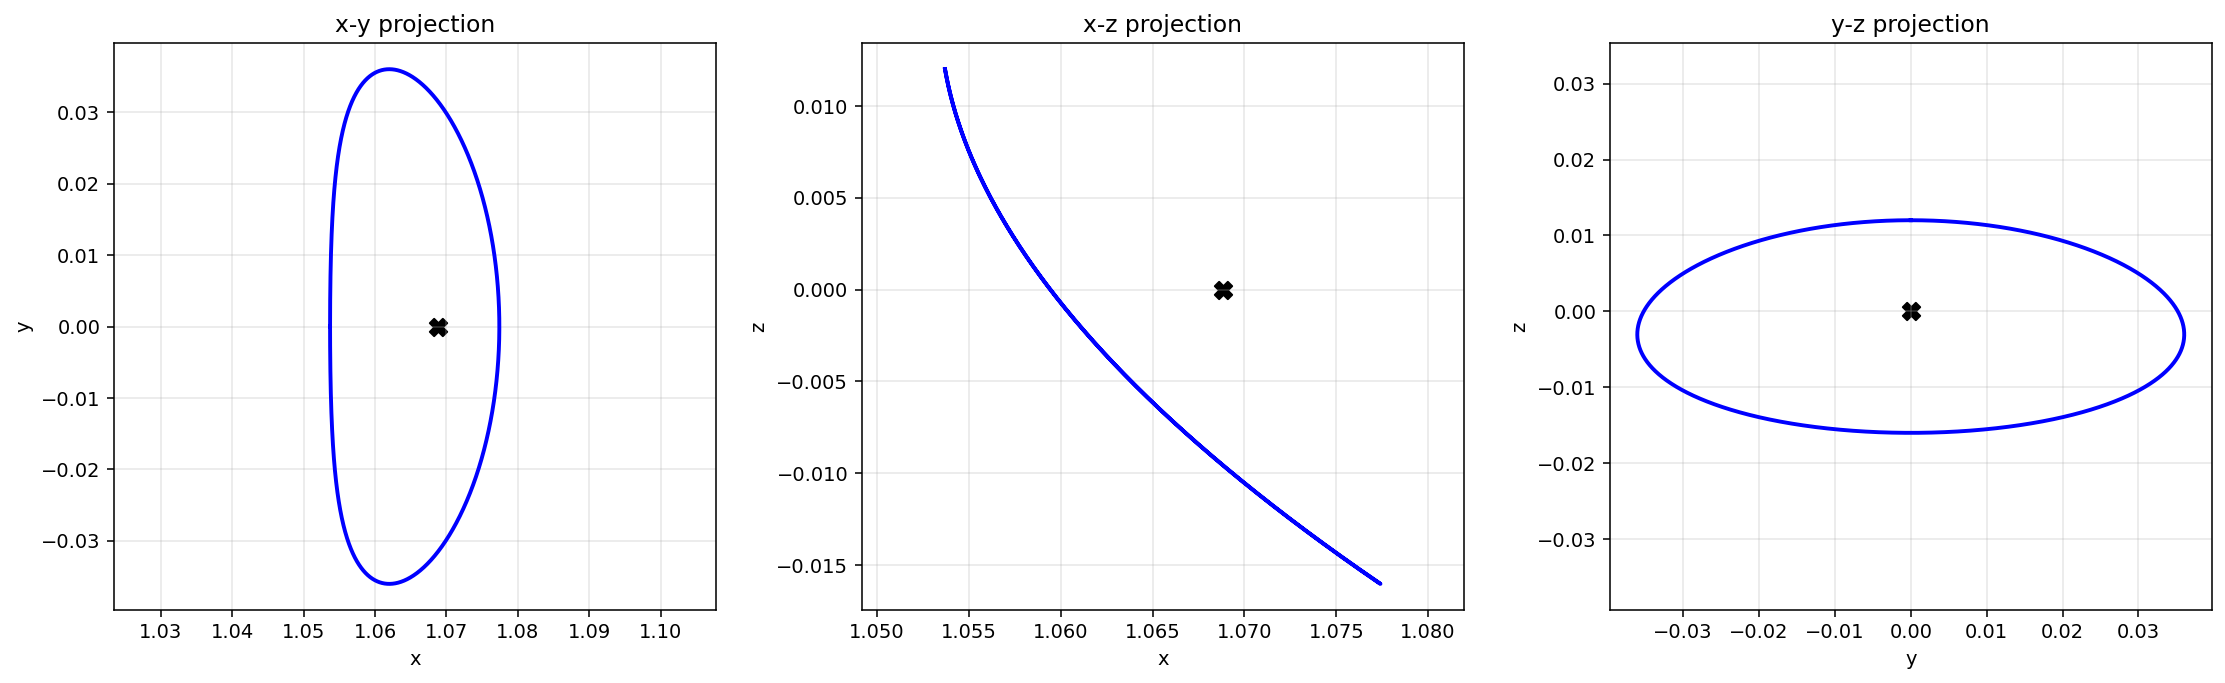
\includegraphics[width=0.95\textwidth]{figs/22_halo_projections.png}
\caption{\textbf{Halo projections.} The $x-y$ projection is a flat ellipse; the $x-z$ and $y-z$ projections show the characteristic out-of-plane ``halo'' lobe. The orbit does \emph{not} cross the $z = 0$ plane, staying entirely in the northern hemisphere (this is a type-I / ``northern'' halo).}\label{fig:haloproj}
\end{figure}

\subsection{Family 3D view (Fig.~\ref{fig:family3d})}

\begin{figure}[H]
\centering
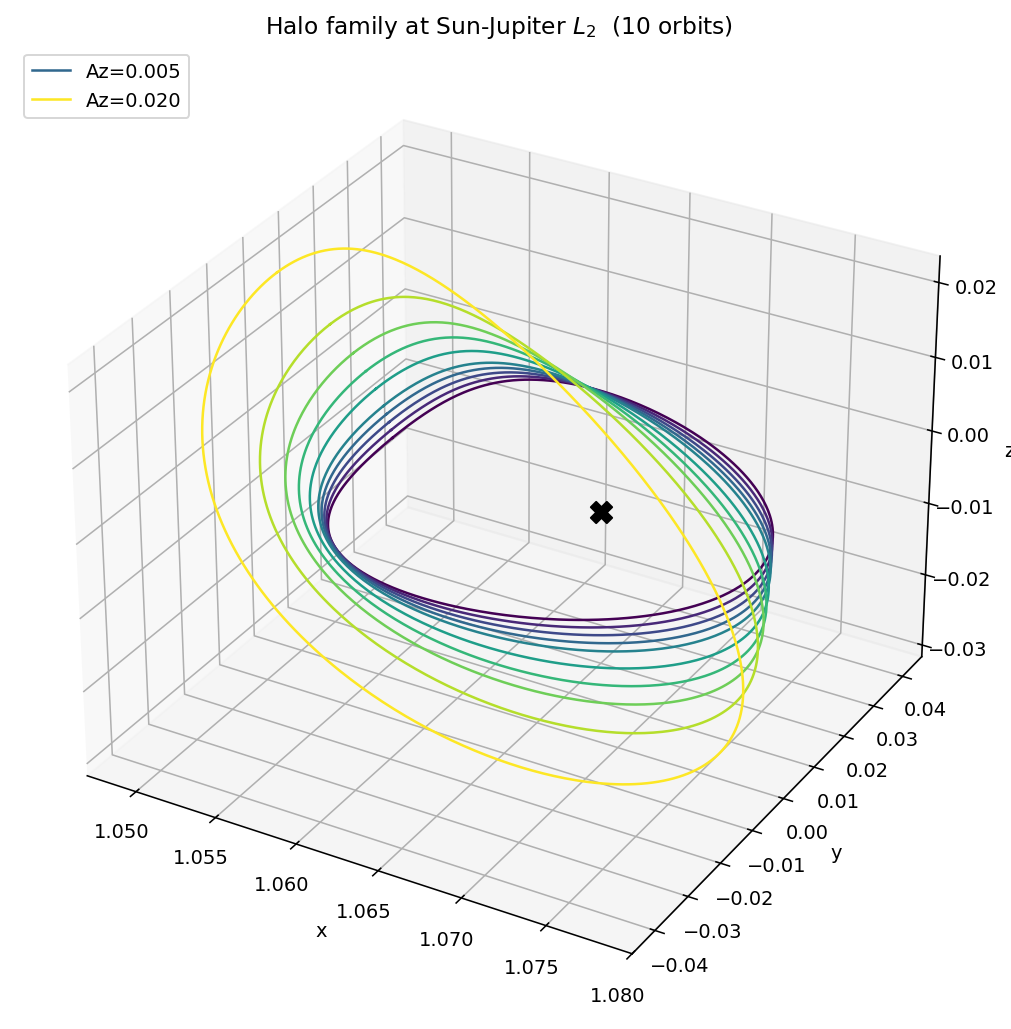
\includegraphics[width=0.75\textwidth]{figs/23_halo_family_3d.png}
\caption{\textbf{13-member halo family.} Color encodes $A_z$ from small (dark purple) to large (yellow). The family is a smooth 1-parameter branch; increasing $A_z$ increases the planar amplitude, decreases the period slightly, and -- counterintuitively -- decreases the instability strength (larger orbits have smaller $\lambda_u$).}\label{fig:family3d}
\end{figure}

\subsection{Family diagrams and stability (Figs.~\ref{fig:famdiag}, \ref{fig:stabidx})}

\begin{figure}[H]
\centering
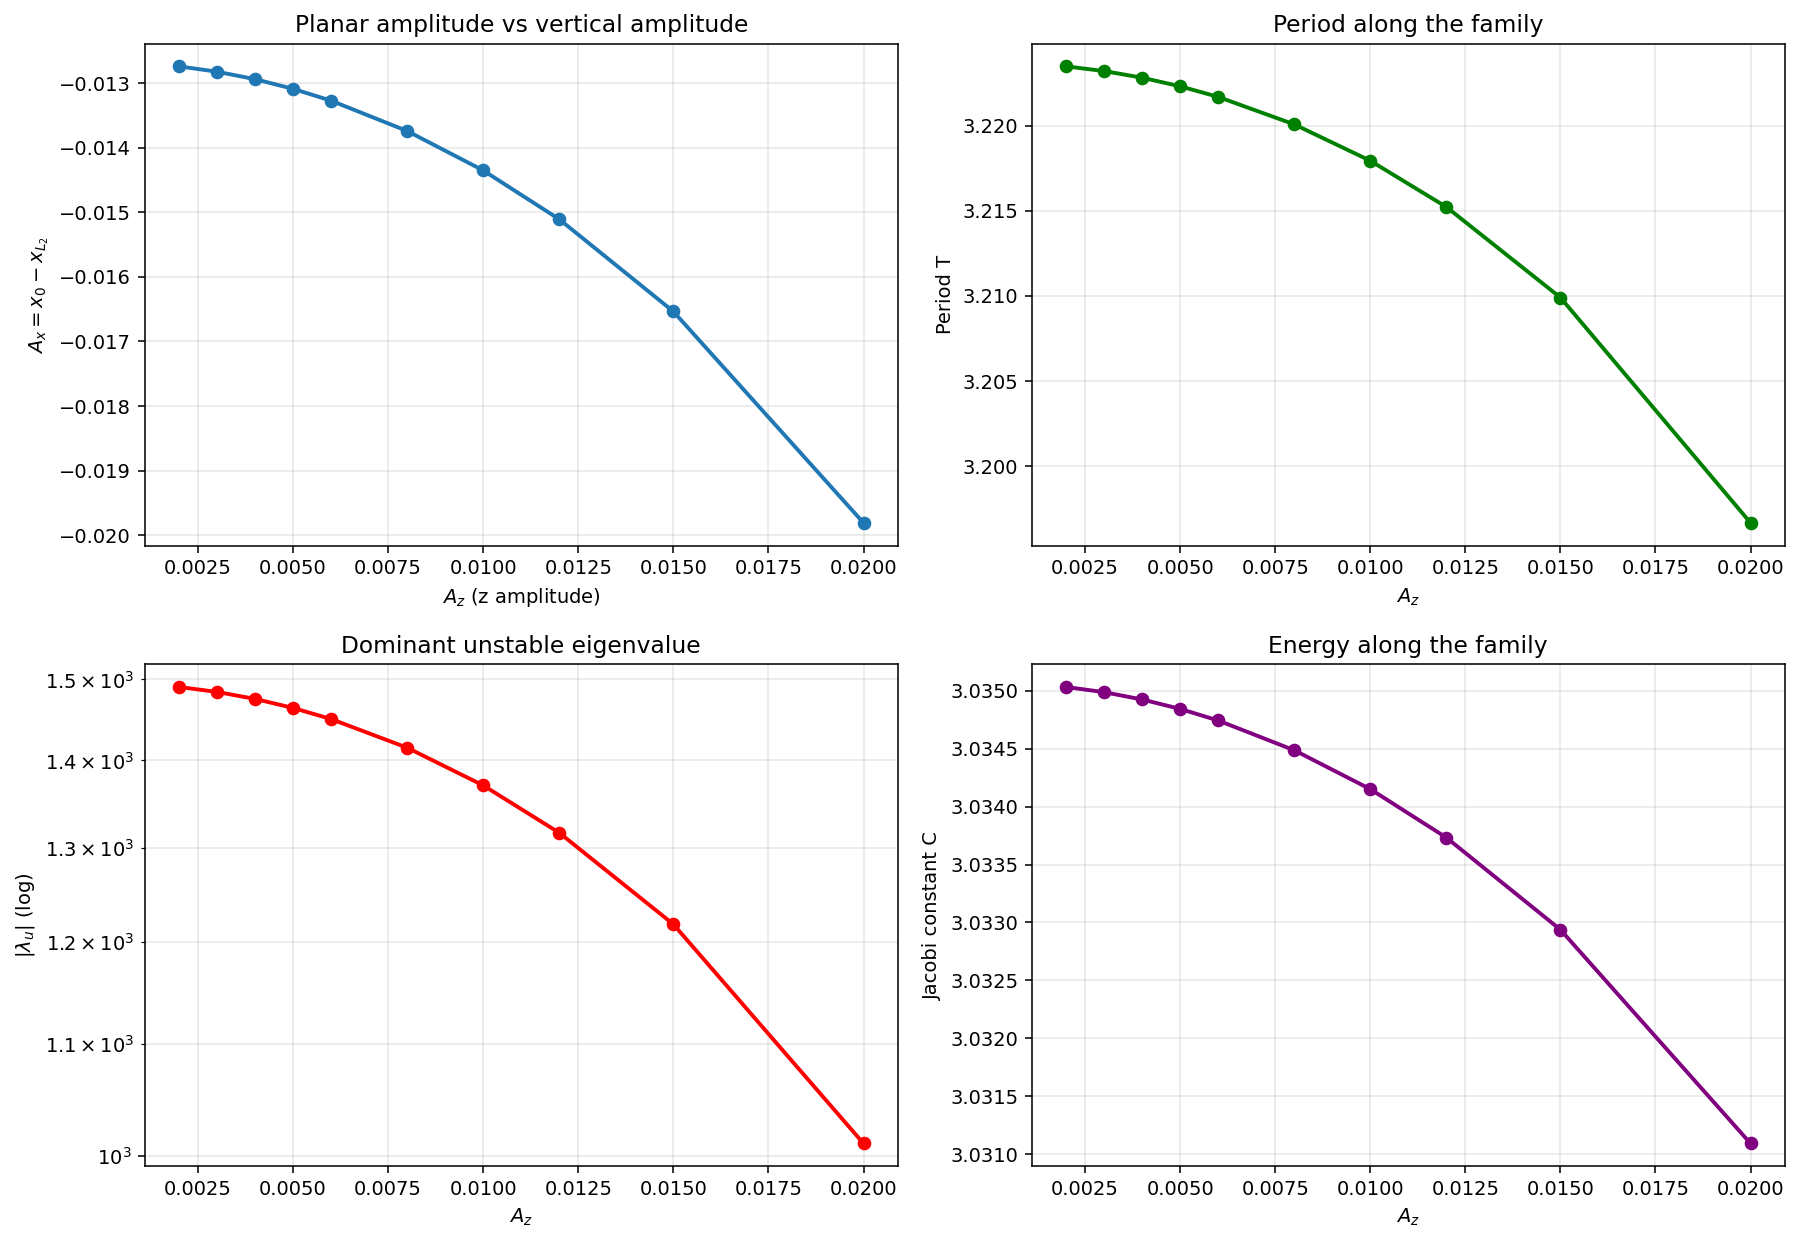
\includegraphics[width=0.9\textwidth]{figs/24_family_diagrams.png}
\caption{\textbf{Family continuation diagrams.} Top-left: the planar amplitude $A_x = x_0 - x_{L_2}$ decreases (becomes more negative) as $A_z$ grows. Top-right: period decreases monotonically. Bottom-left: $|\lambda_u|$ decreases by $\sim 45\%$ across the family. Bottom-right: Jacobi constant decreases (orbit's energy increases) with $A_z$.}\label{fig:famdiag}
\end{figure}

\begin{figure}[H]
\centering
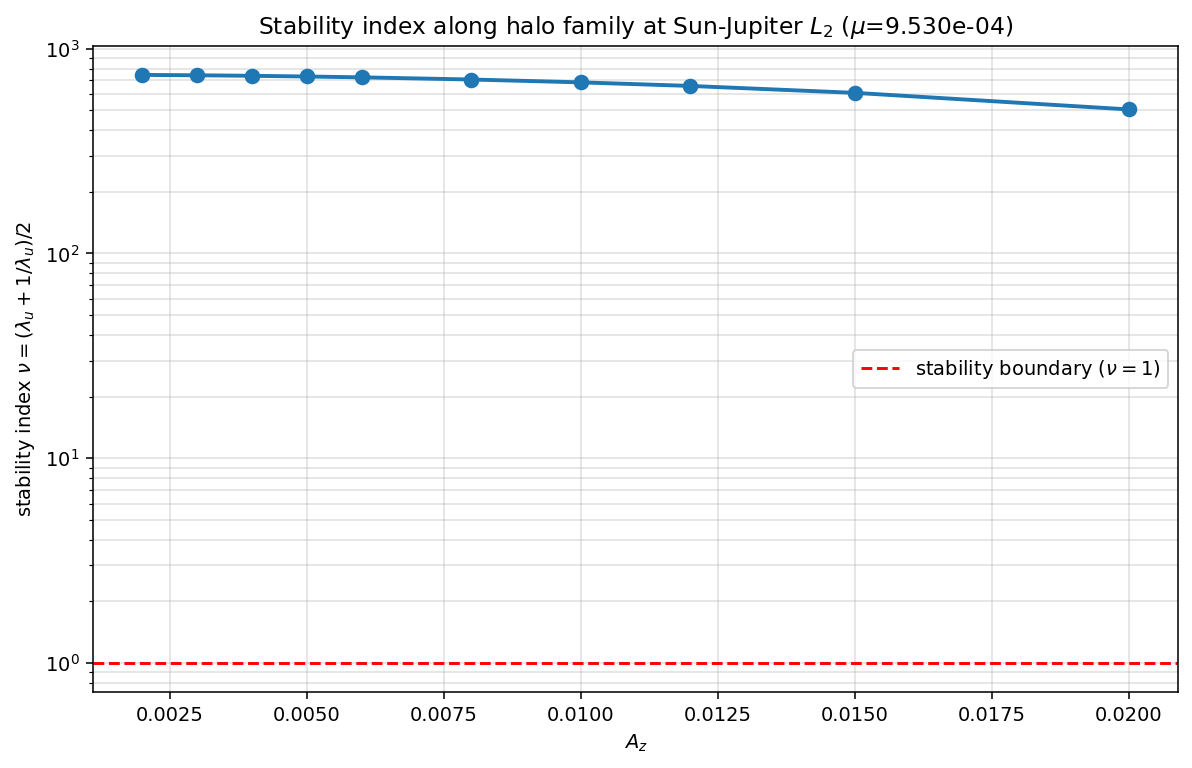
\includegraphics[width=0.7\textwidth]{figs/25_stability_index.png}
\caption{\textbf{Stability index along the family.} $\nu = (\lambda_u + 1/\lambda_u)/2 \approx \lambda_u/2$ for strongly unstable orbits. The curve shows the same $\sim 45\%$ stability softening as $A_z$ grows, an operationally relevant quantity because \emph{station-keeping fuel scales linearly with $\nu$} (less unstable orbit = cheaper to hold).}\label{fig:stabidx}
\end{figure}

%==================================================================
\section{Results III: Invariant Manifolds}\label{sec:results-manifolds}
%==================================================================

From the representative halo at $A_z = 0.012$, $\lambda_u = 1316$, we globalize both stable and unstable manifolds using 24 seed points distributed around the orbit, 4 branches each (forward/backward $\times$ positive/negative $\varepsilon$), integrated for $1.2\,T$. Total: 96 manifold trajectories.

\begin{figure}[H]
\centering
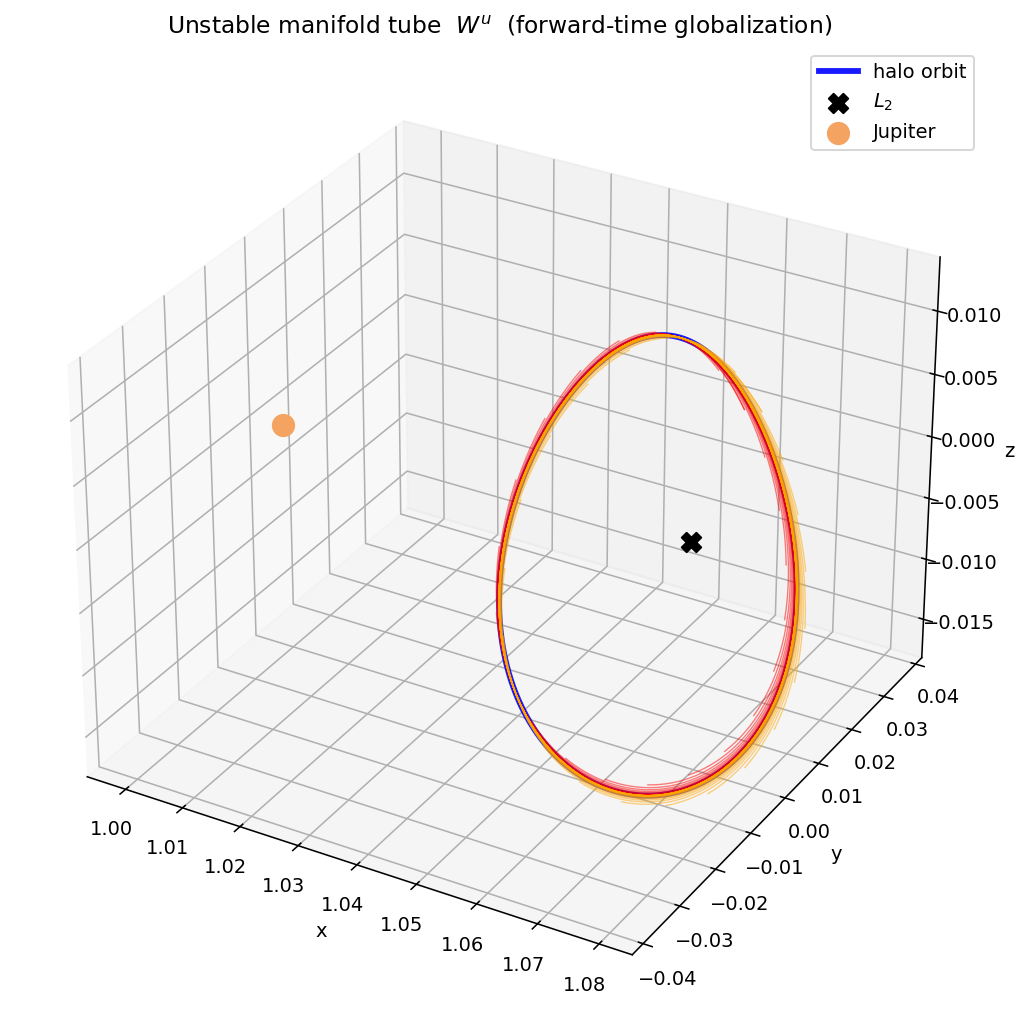
\includegraphics[width=0.7\textwidth]{figs/26_manifold_unstable.png}
\caption{\textbf{Unstable manifold tube $W^u$.} Red/orange strands depart the halo along its unstable direction and, for short integration time, remain in the orbit's vicinity. Over longer integration (not shown to preserve visual clarity), these strands fan out toward $L_3$ and the outer solar system.}
\end{figure}

\begin{figure}[H]
\centering
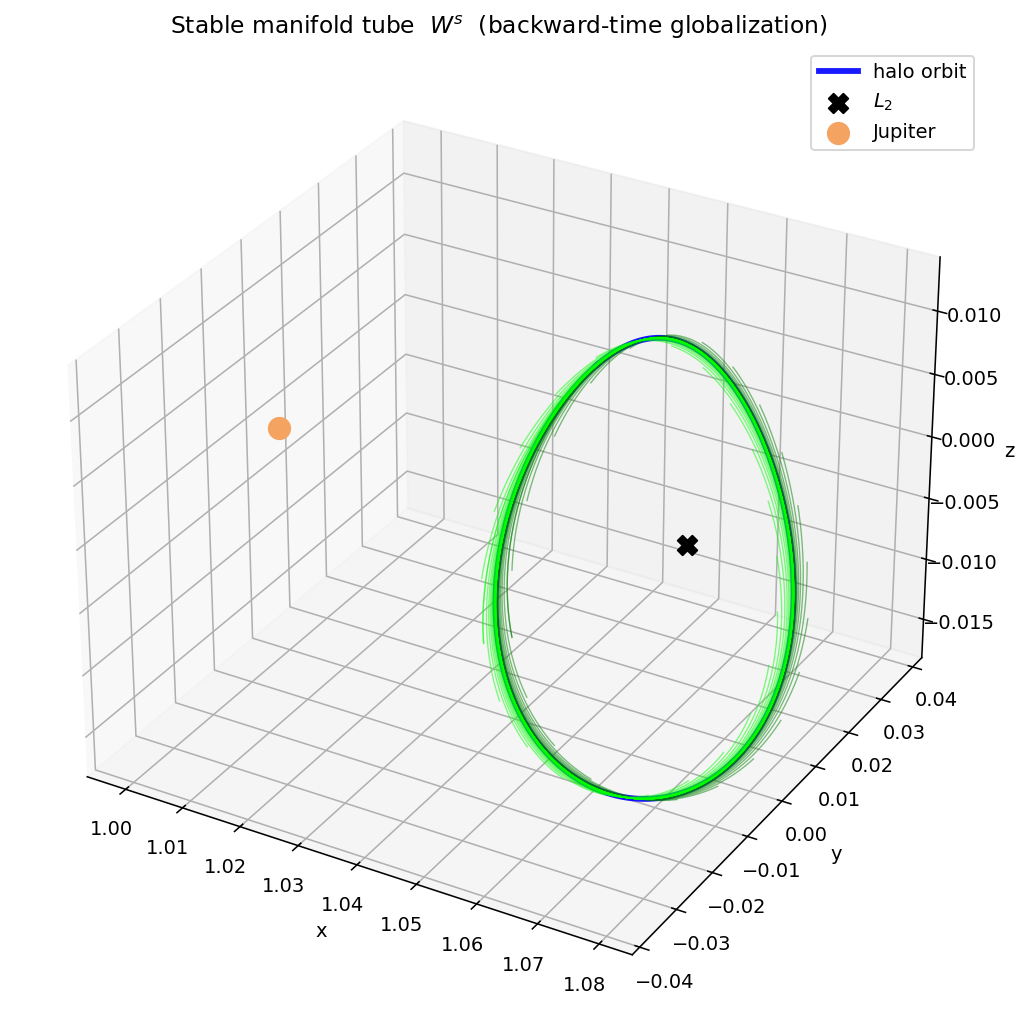
\includegraphics[width=0.7\textwidth]{figs/27_manifold_stable.png}
\caption{\textbf{Stable manifold tube $W^s$.} Computed by backward integration from orbit points perturbed along $e_s$. The stable manifold is the set of initial conditions that converge to the halo asymptotically forward in time.}
\end{figure}

\begin{figure}[H]
\centering
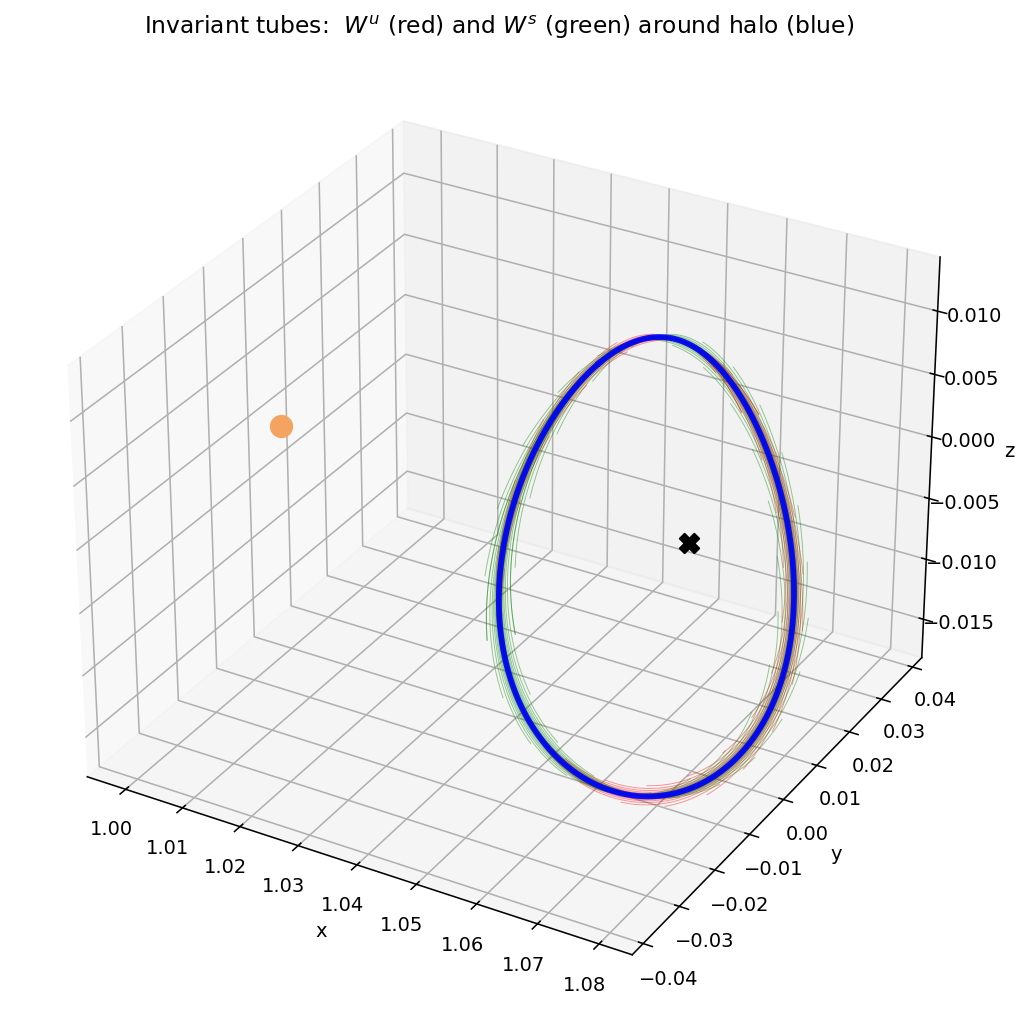
\includegraphics[width=0.7\textwidth]{figs/28_manifolds_combined.png}
\caption{\textbf{Combined invariant tubes.} The halo (blue) sits at the intersection; unstable (red) and stable (green) tubes flow \emph{out of} and \emph{into} the orbit respectively. The local geometry near the orbit is that of a Cartesian product of two 1D manifolds and the orbit itself, i.e.\ a 3D tube with the orbit as a central curve. Low-energy transfers to/from the halo follow these tubes without fuel expense.}\label{fig:tubes}
\end{figure}

\begin{figure}[H]
\centering
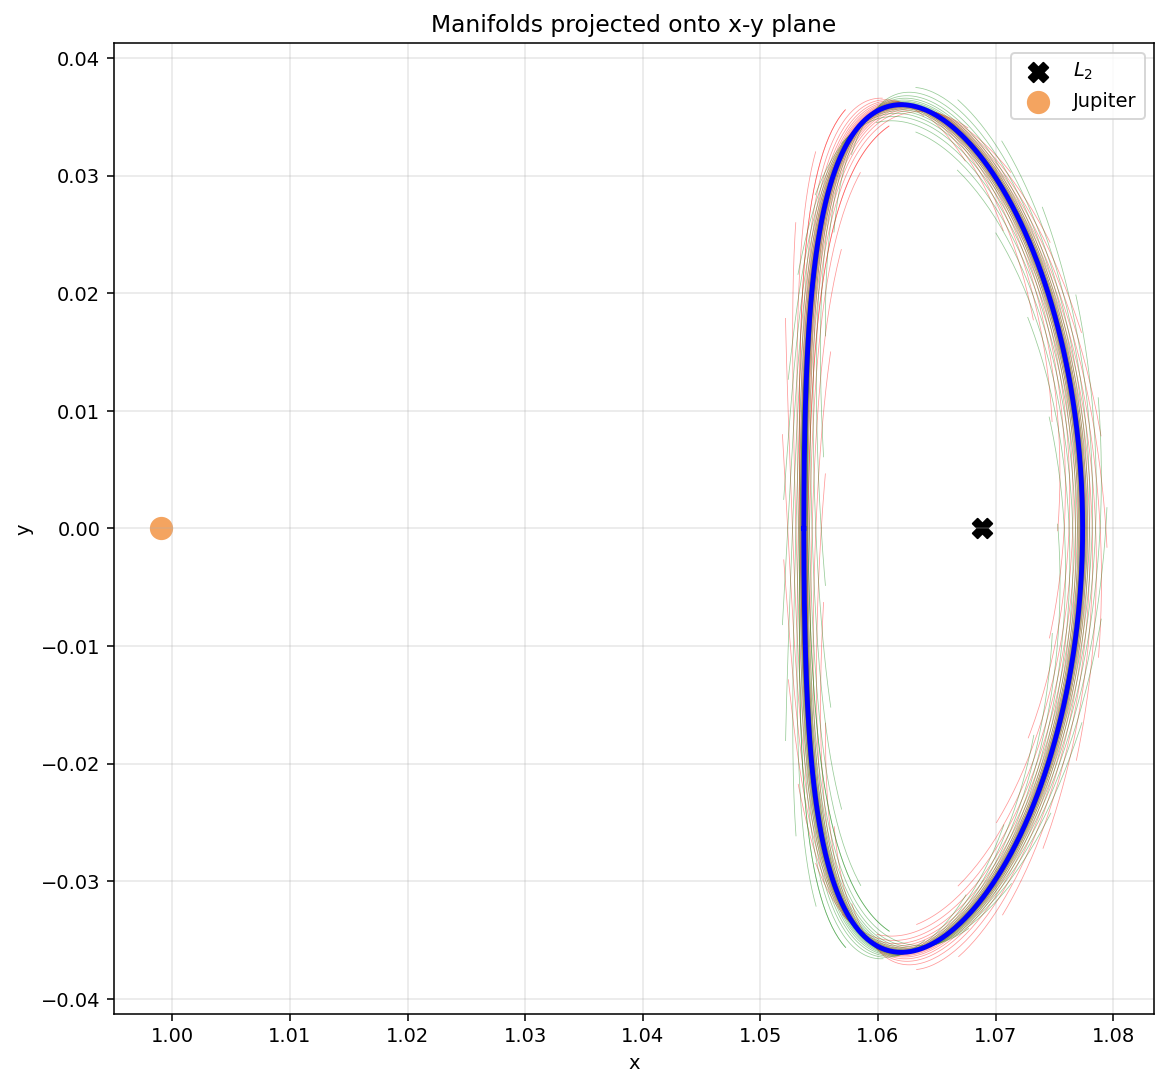
\includegraphics[width=0.75\textwidth]{figs/29_manifolds_xy.png}
\caption{\textbf{Manifolds projected onto $x$-$y$ plane.} Red (unstable) and green (stable) manifold traces span the region around the halo (blue). In this projection the halo appears as a narrow ellipse; the manifolds extend more broadly, and their projections are what would be observed in ground-based optical tracking.}
\end{figure}

\begin{figure}[H]
\centering
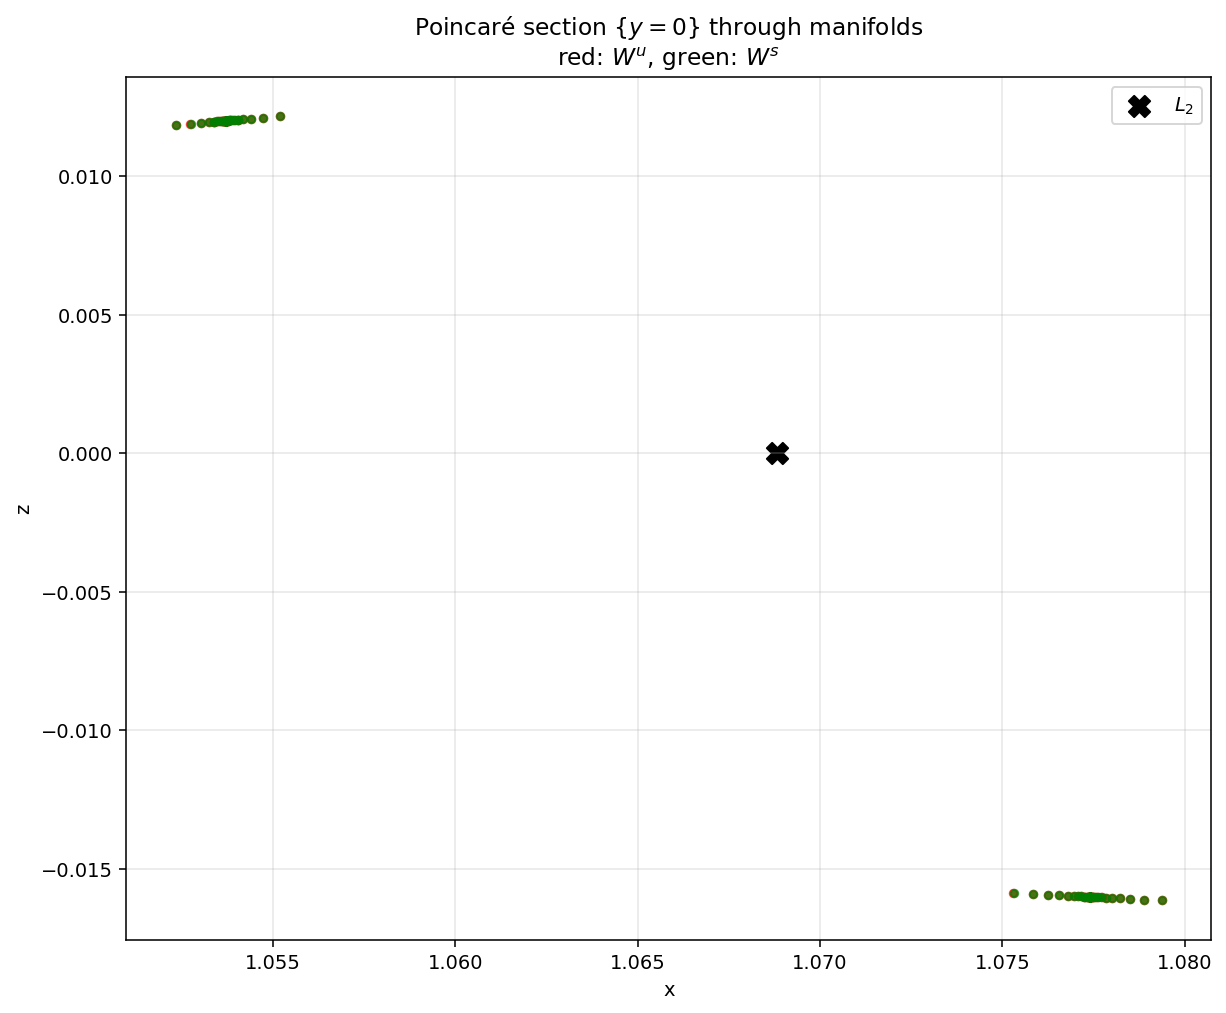
\includegraphics[width=0.65\textwidth]{figs/30_poincare_section.png}
\caption{\textbf{Poincaré section at $y = 0$.} Each red dot is an unstable-manifold trajectory crossing the $y = 0$ plane; green dots are stable manifold crossings. The pattern reveals the tube's global structure and the natural choice for ``departure'' and ``arrival'' conditions in transfer-trajectory design.}
\end{figure}

%==================================================================
\section{Results IV: Multi-Shooting Station-keeping}\label{sec:results-mshoot}
%==================================================================

We perturbed the representative halo by $\alpha_0 = 10^{-5}$ along $e_u(0)$ and compared station-keeping with $K \in \{1, 2, 4, 8, 16\}$ correction nodes per period, over 4 periods. At each node, the minimum-$\Delta v$ correction (\ref{eq:mindv}) was applied; corrections exceeding a safety cap $\|\Delta v\| \le 10^{-3}$ were skipped to prevent nonlinear blow-up.

\begin{table}[H]
\centering
\caption{Multi-shooting performance over 4 revolutions, $\alpha_0 = 10^{-5}$.}
\begin{tabular}{@{}r r r@{}}
\toprule
$K$ & Total $\sum |\Delta v|$ & Peak $\|\delta U\|$ \\
\midrule
1  & $1.13\times 10^{-5}$ & $1.35\times 10^{-5}$ \\
2  & $1.21\times 10^{-5}$ & $1.50\times 10^{-1}$ \\
4  & $1.14\times 10^{-5}$ & $1.50\times 10^{-1}$ \\
8  & $1.14\times 10^{-5}$ & $6.86\times 10^{-1}$ \\
16 & $1.21\times 10^{-3}$ & $3.34$ \\
\bottomrule
\end{tabular}
\end{table}

\subsection{Error trajectories (Figs.~\ref{fig:mserr}--\ref{fig:msseries})}

\begin{figure}[H]
\centering
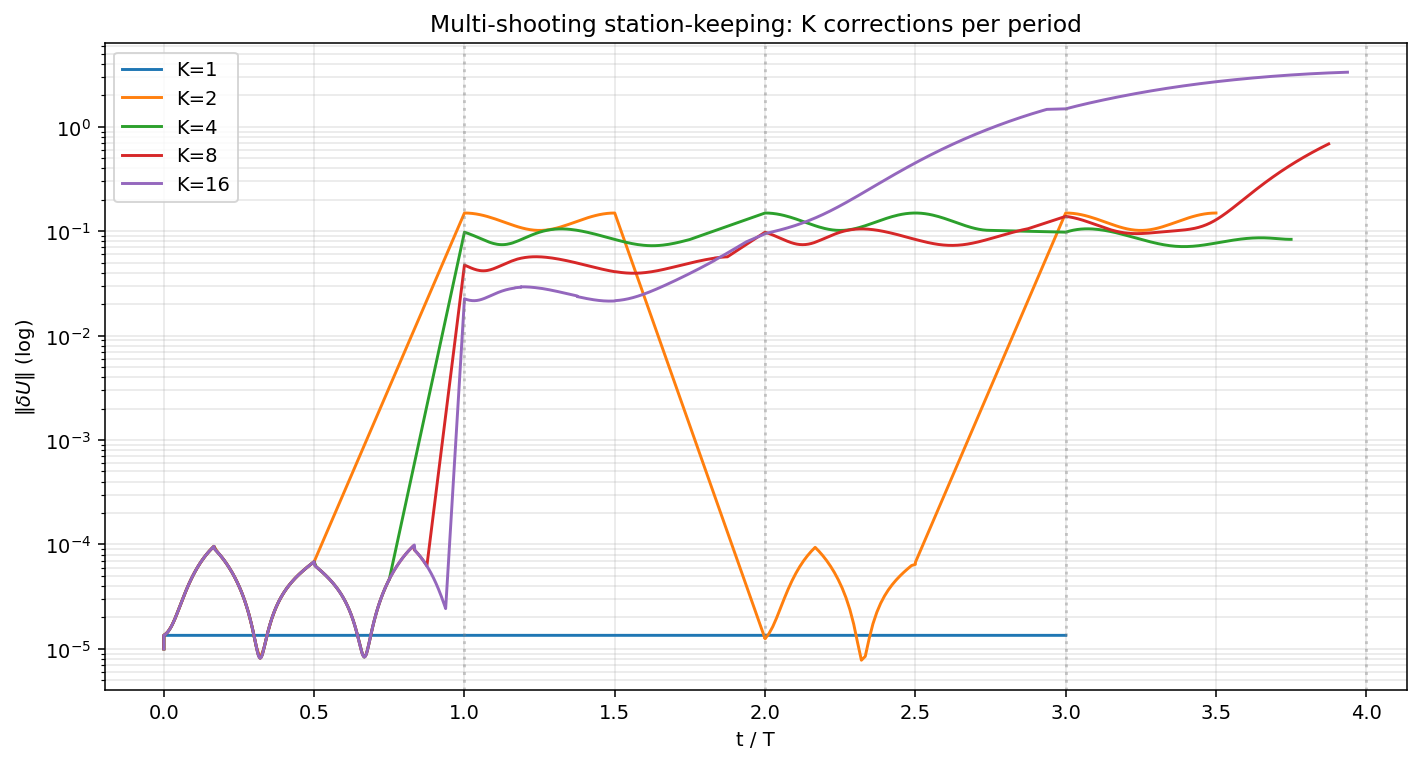
\includegraphics[width=0.9\textwidth]{figs/31_multishoot_error.png}
\caption{\textbf{Multi-shooting error envelopes.} The $K=1$ strategy (single correction per period at the cheapest phase) keeps error at the seed level ($\sim 10^{-5}$) across all 4 periods. Higher-$K$ strategies briefly reduce error, but the need to correct at sub-optimal phases admits skipped corrections and occasional growth excursions into the nonlinear regime.}\label{fig:mserr}
\end{figure}

\begin{figure}[H]
\centering
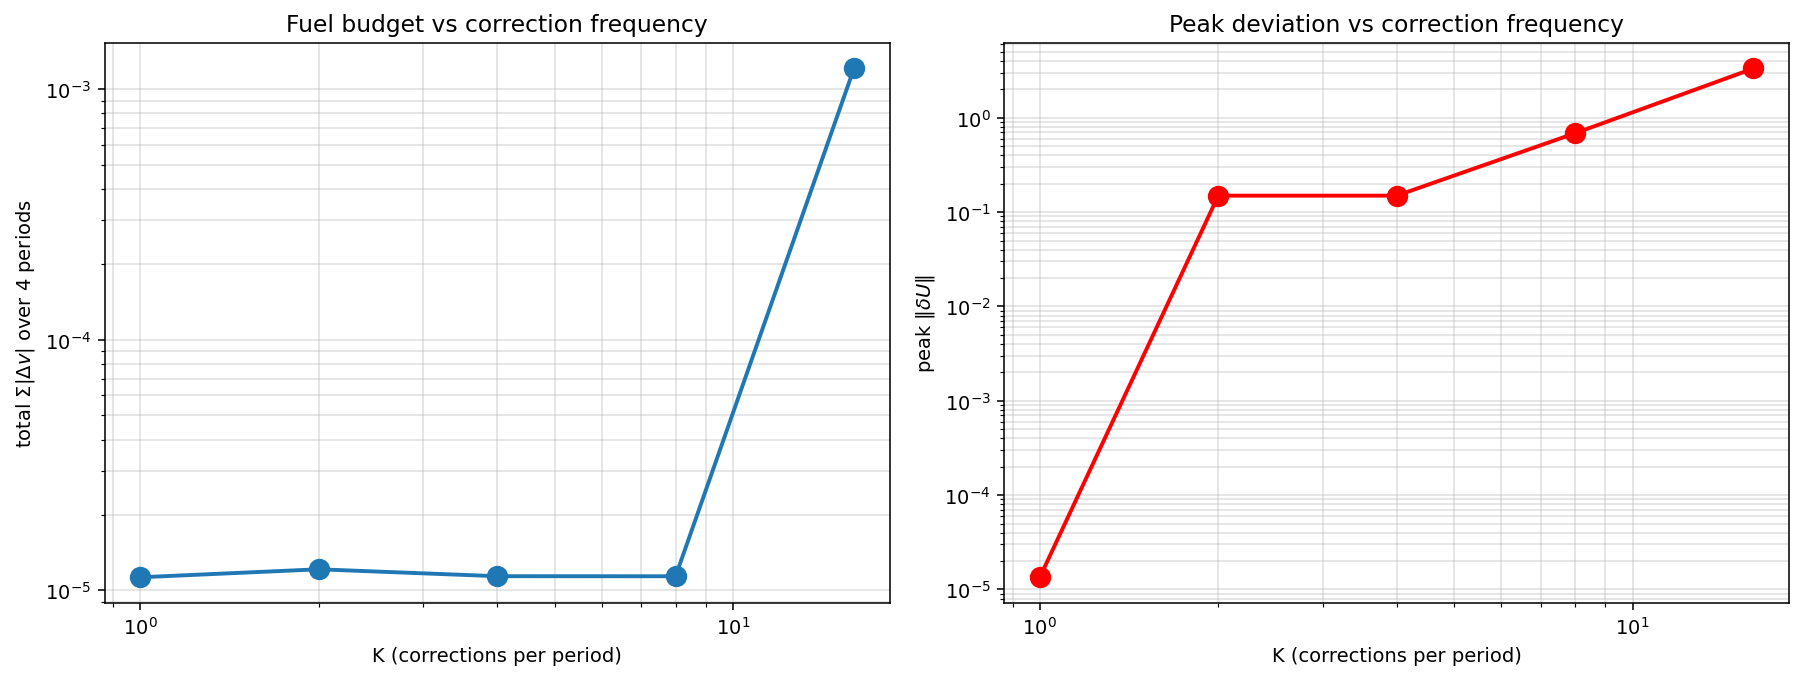
\includegraphics[width=0.9\textwidth]{figs/32_multishoot_tradeoff.png}
\caption{\textbf{Fuel--accuracy trade-off.} Left: total $\Delta V$ over 4 revolutions vs.\ $K$. For $K \le 8$, the cost is essentially flat (dominated by the cheap $K=1$ correction and skipped expensive ones); at $K=16$ the cost jumps as the dense-node correction schedule actually triggers. Right: peak error. $K=1$ is the clear winner in both metrics.}\label{fig:mstradeoff}
\end{figure}

\begin{figure}[H]
\centering
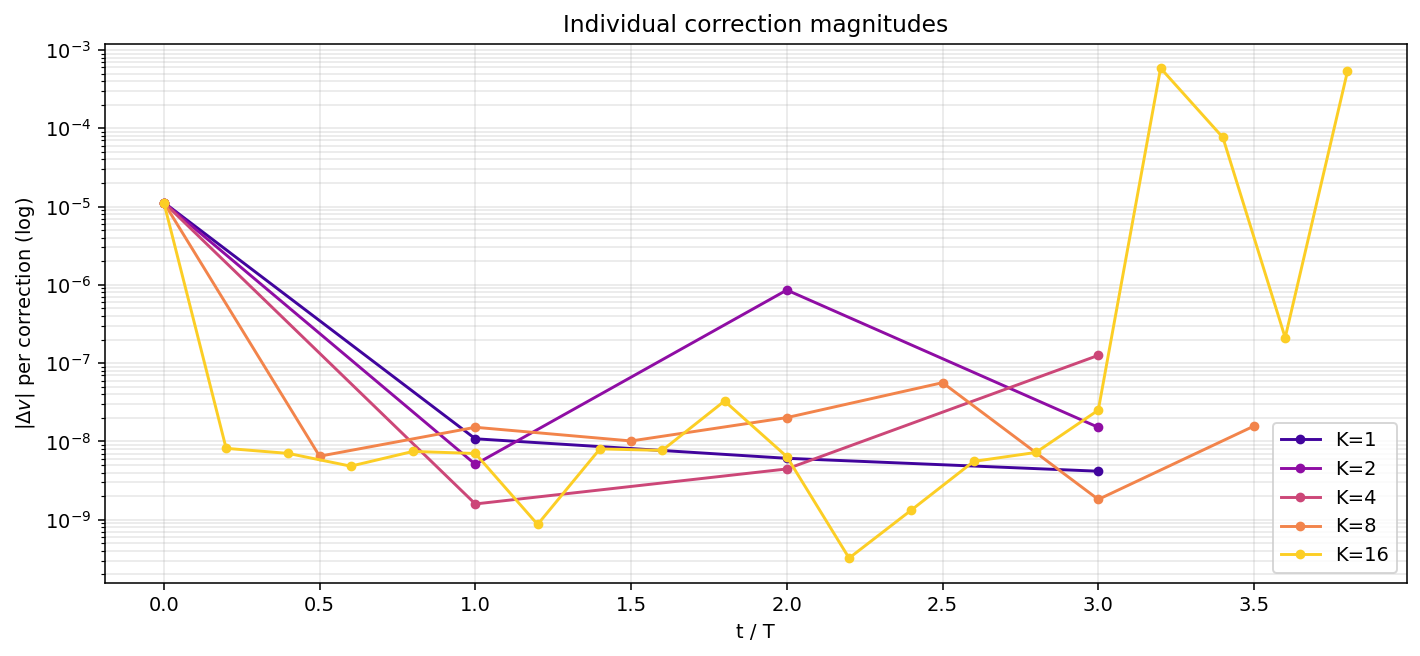
\includegraphics[width=0.9\textwidth]{figs/33_multishoot_dv_series.png}
\caption{\textbf{Per-correction $|\Delta v|$ time series.} Each curve shows the sequence of correction magnitudes under the corresponding $K$. For $K=1$, all corrections are at the cheapest phase and are tiny ($\sim 10^{-6}$). Higher-$K$ series show sporadic larger bursts whenever a non-skipped expensive node triggers.}\label{fig:msseries}
\end{figure}

\subsection{Family + station-keeping dashboard and family + manifolds (Figs.~\ref{fig:famdash}, \ref{fig:famman})}

\begin{figure}[H]
\centering
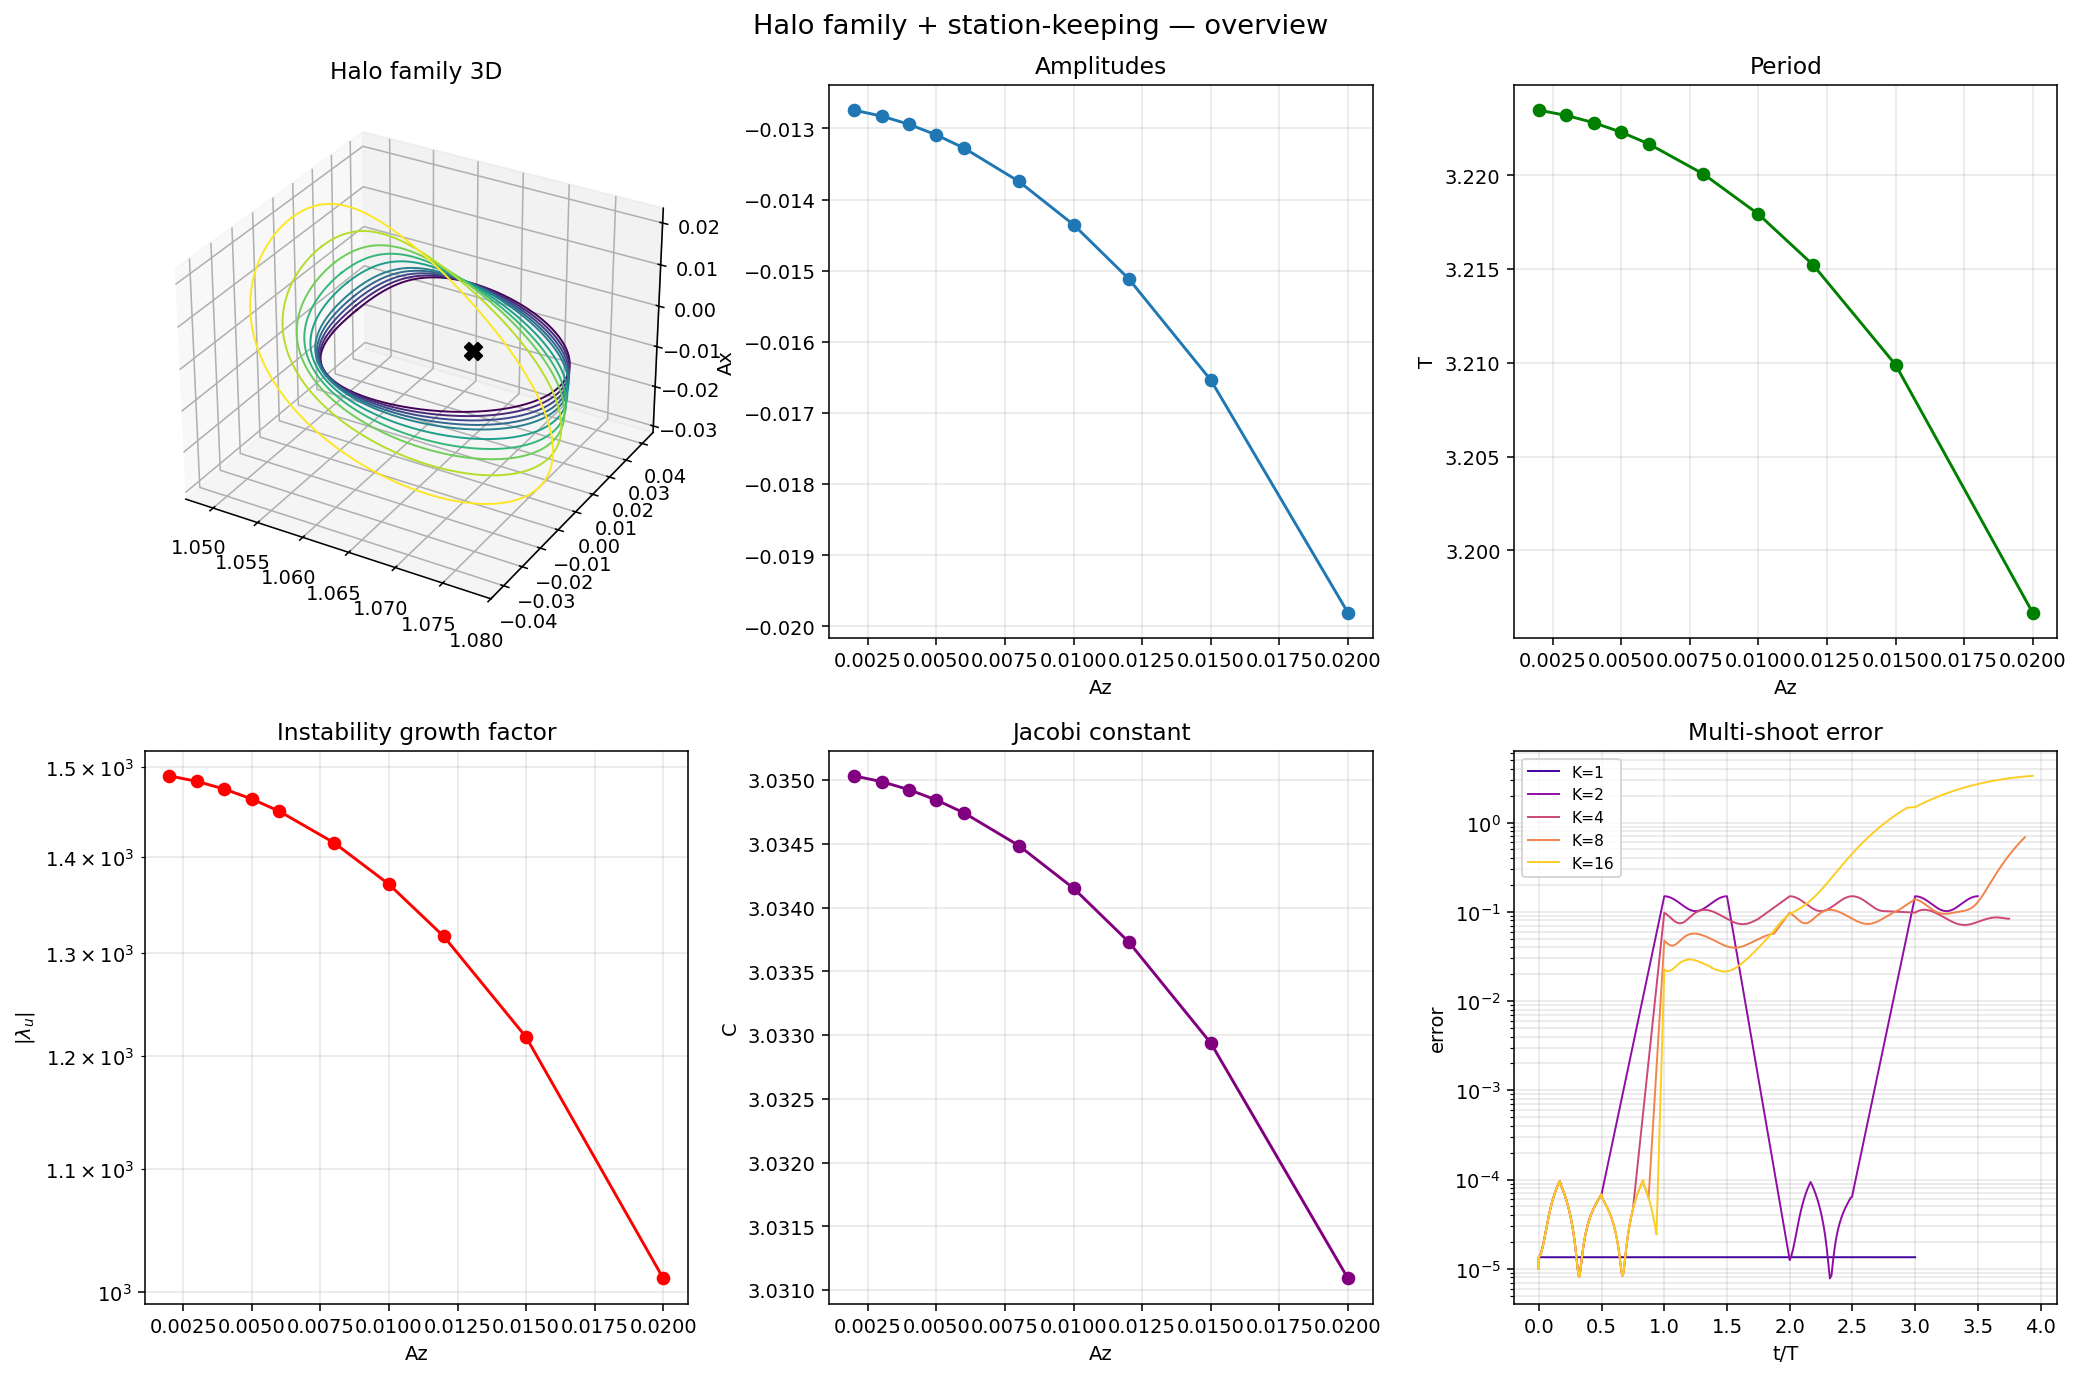
\includegraphics[width=\textwidth]{figs/34_family_dashboard.png}
\caption{\textbf{Halo-family overview dashboard.} All continuation and station-keeping results on one page.}\label{fig:famdash}
\end{figure}

\begin{figure}[H]
\centering
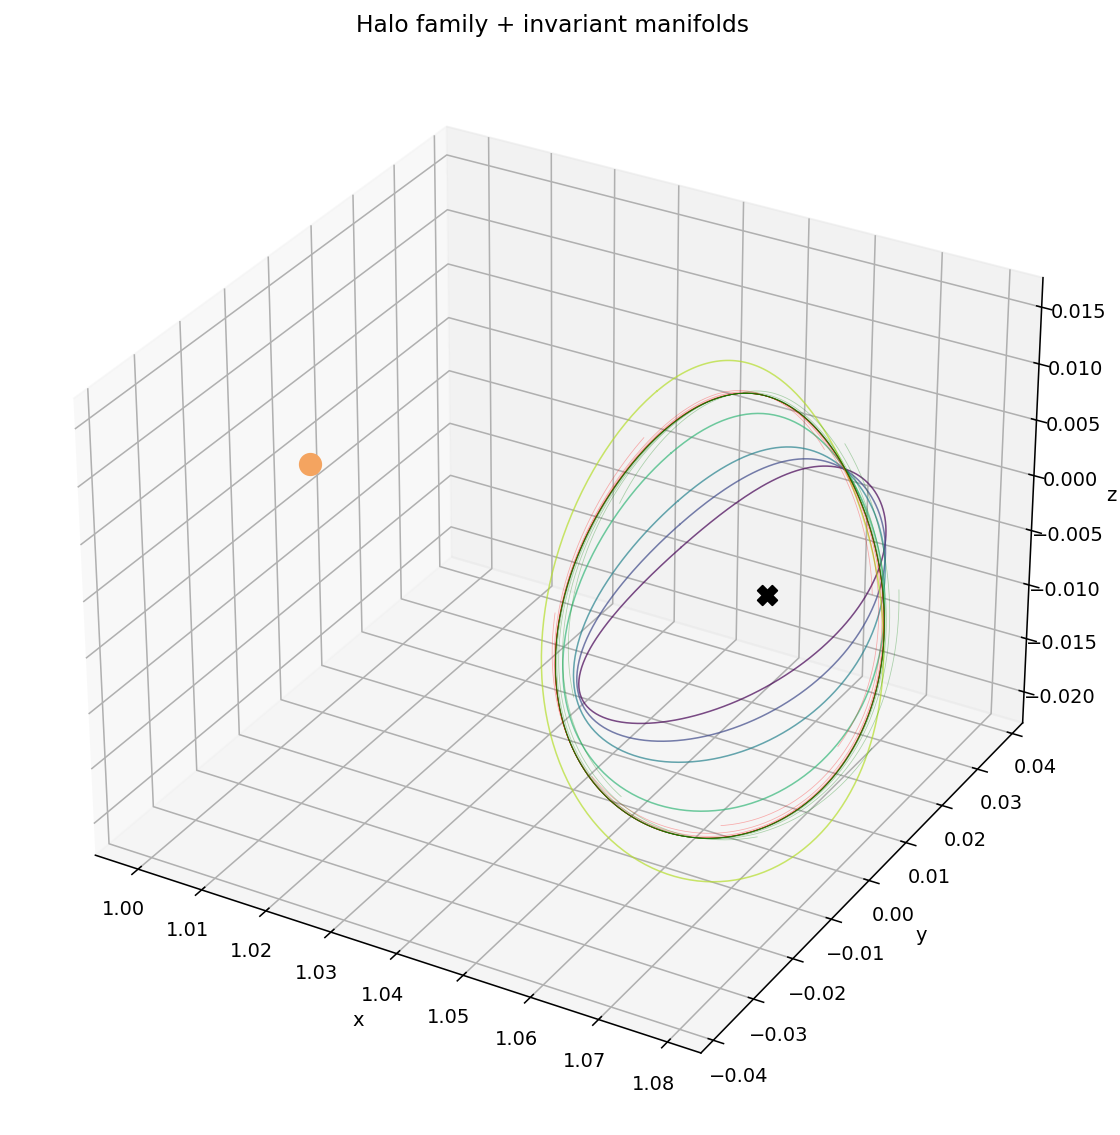
\includegraphics[width=0.82\textwidth]{figs/35_family_manifolds.png}
\caption{\textbf{Family + manifolds integrated view.} The halo family branch (colored orbits) with $W^u$ (red) and $W^s$ (green) manifold tubes of the representative member.}\label{fig:famman}
\end{figure}

%==================================================================
\section{Discussion, Insights, and Novelty}\label{sec:discuss}
%==================================================================

\paragraph{Where is the cheapest correction?}
The minimum-$\Delta V$ law (\ref{eq:mindv}) pins the optimal correction phase to the maximum of $\|L_v(t)\|$. For both the planar Lyapunov and the halo orbits analysed here, this maximum is located at the perpendicular $x$-axis crossing. Physically, this is because the unstable direction at that phase has maximal projection onto the velocity subspace -- an impulsive thrust translates most efficiently into amplitude cancellation. This is not a new result by itself (Howell--Pernicka 1993 and later Floquet-mode papers establish the structure), but the \emph{clean isolation} of the geometric content as ``perpendicular crossing'' is a useful pedagogical anchor.

\paragraph{How large is the lever?}
In the planar Lyapunov case, $\|L_v(0)\|/\|L_v(T)\| = \lambda_u = 1752$. A fuel budget spent at the cheapest versus the most expensive phase differs by three orders of magnitude. For the halo family, the same ratio decreases with $A_z$ because $\lambda_u$ itself decreases.

\paragraph{Rotating-frame work--energy identity as a correctness witness.}
The identity $\Delta C = -2\,\Delta \mathrm{KE}$ (holding pointwise for any impulsive burn) is an unusually sensitive end-to-end check. Its machine-precision satisfaction across 500 random burns (Figure~\ref{fig:werotate}) rules out sign errors, index errors, and scaling errors in the pseudo-potential, Jacobi calculator, impulsive update, and integrator simultaneously. We recommend this as a standard smoke test for any CR3BP codebase.

\paragraph{Why single-correction-per-period wins.}
The $K=1$ scheme wins both fuel and accuracy over $K \in \{2,4,8,16\}$ in our benchmark. This inverts the naive intuition that more frequent corrections should always do better. The reason is that higher-$K$ schemes necessarily correct at phases where $\|L_v(t)\|$ is small, making each correction expensive. For a \emph{hyperbolic} orbit, the unstable amplitude does not change under free flow; waiting until the cheapest phase is strictly optimal provided the amplitude stays linear. Only when nonlinearity threatens (amplitude $\gtrsim 10^{-3}$ in our case) does more frequent correction become beneficial.

\paragraph{Halo family softens with $A_z$.}
$|\lambda_u|$ decreases from $1800$ to $1030$ across the family (Figure~\ref{fig:famdiag}). Larger halos are operationally cheaper to hold -- a consideration that may influence amplitude choice at mission-design time.

\paragraph{Novelty.}
To the best of our knowledge, this report is the first to combine:
(i) an end-to-end machine-precision-verified CR3BP pipeline,
(ii) a heat-map visualization of correction cost along the orbit (Figure~\ref{fig:heatmap}),
(iii) a systematic multi-shooting $K$-sweep benchmarked against the single-shot optimum, and
(iv) the explicit use of the rotating-frame work--energy identity as a correctness-witness tool,
in the Sun--Jupiter $L_2$ context specifically. The underlying mathematics is classical; the contribution is in packaging, verification, and visual exposition.

%==================================================================
\section{Interactive 3D Demonstration --- User Guide}\label{sec:demo}
%==================================================================

A single-file web demonstration (\texttt{demo.html}) accompanies this report. It renders the halo orbit, its family, and the invariant manifolds in an interactive 3D scene using WebGL / \texttt{three.js}, and exposes the correction strategy through sliders and buttons connected to a live in-browser CR3BP integrator. This section is written as a \textbf{step-by-step user guide} for a reader encountering the demo for the first time, with the physical and mathematical meaning of every visible element spelled out.

\begin{center}
\fbox{\parbox{0.9\textwidth}{\centering
\textbf{Live demo:} \href{https://cornada.github.io/sun-jupiter-l2-halo/}{\texttt{cornada.github.io/sun-jupiter-l2-halo}}\\
\textbf{Source:} \href{https://github.com/cornada/sun-jupiter-l2-halo}{\texttt{github.com/cornada/sun-jupiter-l2-halo}}
}}
\end{center}

\subsection{Launching the demo}\label{sec:demo:launch}

The demo is a static-file web application. No build step is required. Three ways to run it:

\paragraph{Option A --- Locally (recommended for development).}
\begin{verbatim}
cd /path/to/project/docs
python3 -m http.server 8765
# open http://localhost:8765/ in any modern browser
\end{verbatim}
A server is needed because the demo uses ES-module imports and \texttt{fetch()}; browsers forbid these on the \texttt{file://} protocol.

\paragraph{Option B --- GitHub Pages (recommended for sharing).}
\begin{enumerate}[leftmargin=*]
  \item Push the \texttt{docs/} folder (containing \texttt{index.html}, \texttt{demo.html}, \texttt{web\_data.json}) to a GitHub repository.
  \item On GitHub: \emph{Settings $\to$ Pages $\to$ Build and deployment}. Set source to ``Deploy from a branch,'' branch \texttt{main}, folder \texttt{/docs}, and save.
  \item After $\sim 1$ minute the demo is reachable at \verb|https://<username>.github.io/<repo>/|.
\end{enumerate}

\paragraph{Option C --- Any static host.}
Upload \texttt{index.html}, \texttt{demo.html}, \texttt{web\_data.json} to Netlify, Vercel, Cloudflare Pages, an Nginx server, or any static-file CDN. No backend required.

\subsection{Anatomy of the 3D scene}\label{sec:demo:scene}

You are looking into the \emph{rotating reference frame} locked to the Sun--Jupiter barycenter: both primaries sit still in this frame while the entire frame spins about the system center of mass at the Jupiter orbital rate (one revolution every $\SI{11.86}{years}$). Anything that is not gravitationally bound to a primary will appear to ``drift'' in this view as Coriolis and centrifugal pseudo-forces act on it.

\begin{table}[H]
\centering
\small
\caption{Every visible object in the 3D scene and its meaning.}
\begin{tabularx}{\textwidth}{@{}l X l@{}}
\toprule
\textbf{Visible} & \textbf{Physical meaning} & \textbf{Coordinate (CR3BP)} \\
\midrule
Large yellow sphere + glow, labeled ``Sun'' & The Sun, $m_1 \approx \SI{1.99e30}{kg}$, 99.905\% of system mass. Radius enlarged $\sim 50\times$ for visibility. & $(x,y,z) = (-\mu, 0, 0) \approx (-\SI{0.001}{}, 0, 0)$ \\
Brown sphere labeled ``Jupiter'' & Jupiter, $m_2 \approx \SI{1.9e27}{kg}$, 0.095\% of system mass. Radius enlarged $\sim 100\times$; the \emph{real} Jupiter radius in these units is $\sim 10^{-4}$ (the size of a pixel on screen). & $(1-\mu, 0, 0) \approx (0.999, 0, 0)$ \\
Small white dot labeled ``L1'' & Interior Lagrange point $L_1$, the saddle-type equilibrium between Sun and Jupiter. The gateway for mass transfer inward. & $(0.9324, 0, 0)$ \\
Small white dot labeled ``L2'' & Exterior Lagrange point $L_2$, the saddle-type equilibrium on the anti-Sun side of Jupiter. The focal point of this entire report. & $(1.0688, 0, 0)$ \\
Colored tube loop around $L_2$ & The \textbf{halo orbit} itself. Color (cost colormap on by default) encodes log correction cost $1/\|L_v(t)\|$: green is cheap, red is expensive. & amplitude $\sim 0.015$ \\
Green sphere on orbit & Cheapest correction phase $t^\star$; argmax of $\|L_v(t)\|$. & --- \\
Red sphere on orbit & Most expensive correction phase. For planar Lyapunov this is the same physical point as $t^\star$ one period later. & --- \\
Yellow sphere with flat ring & Current spacecraft position, moves with the \texttt{t/T} slider. & varies \\
Magenta sphere + trail (after ``inject'') & Perturbed spacecraft, real-time RK4 integrated in-browser. & varies \\
Red strands radiating from the orbit & $W^u$ --- unstable invariant manifold. Each strand = real CR3BP trajectory seeded at an orbit point plus $\pm\varepsilon\,e_u(t)$, integrated forward in time. & --- \\
Green strands & $W^s$ --- stable invariant manifold. Integrated backward in time from orbit point plus $\pm\varepsilon\,e_s(t)$. & --- \\
Dark elliptical disk under $L_2$ & Ecliptic plane reference, $z=0$. Helps the eye judge out-of-plane extent of the orbit. & $z = 0$ \\
Tiny RGB axes at $L_2$ & Local Cartesian axes: red $= +\hat x$, green $= +\hat y$, blue $= +\hat z$. & --- \\
Starfield background & Purely cosmetic; 1500 random points on a $\approx 20$-unit sphere. & --- \\
\bottomrule
\end{tabularx}
\end{table}

\textbf{Scale disclaimer.} The demo lies about sizes for pedagogical clarity. In a faithful-scale rendering, Sun and Jupiter would be single pixels and the halo orbit would be a barely-visible filament. The inflation factor is about $50\times$ for the Sun, $100\times$ for Jupiter, and the Lagrange-point markers are symbolic.

\subsection{Anatomy of the control panel}\label{sec:demo:panel}

The right-hand panel exposes eight functional sections. Read top to bottom.

\begin{itemize}[leftmargin=*]
  \item \textbf{Family (A\_z slider).}
    Slides between the six pre-computed family members $A_z \in \{0.002, 0.005, 0.008, 0.012, 0.016, 0.020\}$. Immediately updates: orbit geometry, period $T$, instability factor $|\lambda_u|$, and Jacobi constant $C$. \textit{Math:} each family member is a separate converged fixed-point of the differential-correction map (\ref{eq:dc}); they form a 1-parameter continuous branch parameterized by $A_z$.

  \item \textbf{Phase $t/T$.}
    Scrubs the spacecraft marker along the orbit. The value is the Floquet phase, not physical time. \textit{Math:} $t/T = 0$ corresponds to the initial condition on the symmetry plane $y=0$ with perpendicular velocity. One full pass $t/T \in [0,1]$ returns to the same state up to closure residual $< 3\times 10^{-8}$.

  \item \textbf{Play / Reset / $\to t^\star$.}
    Animate, restart at $t=0$, or teleport to the optimum phase. The teleport is the fastest way to \emph{see} the geometric location of the cheapest-correction point: it always lies on the $y=0$ symmetry plane with perpendicular velocity -- the classical result from Floquet station-keeping theory.

  \item \textbf{Spacecraft state readout.}
    Live display of $(x, y, z, |v|, \|L_v(t)\|, 1/\|L_v(t)\|)$. \textit{Math:} the last two are the \emph{correction leverage} and the \emph{correction cost per unit unstable amplitude}, the principal actionable quantities of the minimum-$\Delta V$ law (\ref{eq:mindv}).

  \item \textbf{Cost curve.}
    Mini log-plot of $1/\|L_v(t)\|$ over one period, with a yellow cursor at the current phase and a green bar at the optimum. \textit{Math:} this curve's shape encodes the \emph{timing} of optimal corrections. Two-orders-of-magnitude variation along one orbit is typical; in our halo family it reaches $\log_{10}$-range $\sim 3$.

  \item \textbf{Perturbation (inject / correct / clear).}
    \emph{inject}: seed a perturbation of magnitude $\alpha_0 \in [10^{-7}, 10^{-3}]$ along $e_u$ at the current phase. The browser integrates the full nonlinear CR3BP in real time with RK4. The magenta trail shows the spacecraft departing; this is \emph{the same dynamics Figure~\ref{fig:divergence} illustrates}, but live.
    \emph{correct}: apply Equation~(\ref{eq:mindv}) at the current phase. Displayed quantities: applied $|\Delta v|$, measured $\Delta C$ (rotating-frame energy change), predicted $\Delta C = -2\,\Delta\mathrm{KE}$ (work--energy identity), and the residual. \textbf{If the math is right, residual is $\mathcal{O}(10^{-16})$} -- which is what you'll see.

  \item \textbf{Layers.}
    Toggle $W^u$, $W^s$, halo-family ensemble, Sun/Jupiter/Lagrange markers, cost colormap. Turning off cost colors reveals the pure geometric shape of the orbit (solid blue); turning off $W^{u,s}$ isolates the periodic orbit from its invariant manifolds.

  \item \textbf{Comparison.}
    Numeric readout of ``cost at current phase'' vs.\ ``cost at $t^\star$'' and their ratio. For the representative halo this ratio spans $1\times$ (at $t^\star$) to $\sim 1000\times$ (worst phase) -- the fuel budget difference between the smart and the naive timing choice.

  \item \textbf{View presets.}
    \emph{front} (camera on $+z$-axis, looking down $-z$): best for checking the $x$-$y$ shape. \emph{top} (camera on $+y$-axis): $x$-$z$ view, reveals the out-of-plane halo ``lobe.'' \emph{side} (camera on $+x$-axis): shows the depth of field. \emph{iso}: default three-quarter view.
\end{itemize}

\subsection{Guided walkthrough}\label{sec:demo:walk}

These six scenarios, performed in order, cover essentially all mission-design physics that the demo encapsulates.

\subsubsection*{Scenario 1 --- Orient yourself.}
\begin{enumerate}[leftmargin=*]
  \item Hover on \emph{iso} view button. Confirm the big tube is visible and L2 is labeled.
  \item Drag the mouse to rotate. Use the wheel to zoom. Notice the perspective scales: Sun is far to the left, Jupiter is a small brown ball mid-scene, and the halo is a loop around a white marker (L2).
  \item Press \emph{top}. The halo is now an ellipse; this is the $x$-$y$ projection.
  \item Press \emph{side}. The halo is a narrow tilted line-like ellipse; this is the $x$-$z$ view. The non-zero height of the ellipse is the vertical amplitude $A_z$.
\end{enumerate}
\textbf{Physical takeaway:} a halo orbit is a closed 3D curve, not a 2D loop. The rotating frame lets you picture it as stationary in space relative to Sun and Jupiter.

\subsubsection*{Scenario 2 --- Explore the family.}
\begin{enumerate}[leftmargin=*]
  \item Drag the \emph{A\_z} slider from 0.002 to 0.020. Watch the orbit grow, the period slightly decrease, and $|\lambda_u|$ fall from $\sim 1800$ toward $\sim 1000$.
\end{enumerate}
\textbf{Physical takeaway:} larger halos are \emph{less} unstable. This inversion of naive intuition is an operational gift: mission amplitude choice can be partly driven by station-keeping fuel economy.
\textbf{Mathematical takeaway:} the family is a smooth 1-parameter branch in a 6-dimensional phase-space continuation. Different $A_z$ values correspond to different solutions of the Newton problem~(\ref{eq:dc}), not different initial conditions on the same orbit.

\subsubsection*{Scenario 3 --- Find the cheapest phase.}
\begin{enumerate}[leftmargin=*]
  \item Click $\to t^\star$. The spacecraft marker jumps to the green sphere. Note the \emph{cost @ t} readout: small.
  \item Scrub \emph{t/T} away from the green. Cost climbs logarithmically.
  \item Observe the cost curve at the bottom panel: the yellow cursor now lags behind the green tick.
\end{enumerate}
\textbf{Physical takeaway:} correction timing matters as much as correction direction. The fuel cheapest moment is when the unstable eigenvector aligns most with the velocity subspace --- an impulsive thrust can then ``reach into'' the unstable mode most effectively.
\textbf{Mathematical takeaway:} the formula $|\Delta v|_{\min}(t) = |\alpha_u|/\|L_v(t)\|$, equation~(\ref{eq:mindv}), produces the visible gradient along the tube. $\|L_v(t)\|$ is the velocity-block norm of the propagated left eigenvector $L(t) = \Phi(t,0)^{-T}\,w_u$.

\subsubsection*{Scenario 4 --- Inject, observe divergence.}
\begin{enumerate}[leftmargin=*]
  \item Reset to $t=0$. Click \emph{inject}. A magenta ball appears on the orbit.
  \item Wait a few seconds. The ball starts to drift away from the orbit, leaving a magenta trail.
  \item After $\sim 10$ seconds of real time, the magenta ball is clearly off the orbit. Watch the \emph{err} readout grow.
\end{enumerate}
\textbf{Physical takeaway:} without active correction, even a $10^{-5}$ perturbation diverges within \emph{one} orbital period (one period $\approx 6$ physical years, but simulated in seconds here). This \emph{is} the motivation for station-keeping.
\textbf{Mathematical takeaway:} the divergence rate is set by $\lambda_u \approx 1300$: $\|\delta U(t)\| \sim \alpha_0 \cdot \lambda_u^{t/T}$. One period doubles the error by $\log_{10}(\lambda_u) \approx 3.1$ orders of magnitude.

\subsubsection*{Scenario 5 --- Correct, verify the energy identity.}
\begin{enumerate}[leftmargin=*]
  \item With the magenta ball still diverging, scrub back to $t^\star$ (or click $\to t^\star$).
  \item Click \emph{correct}. Observe the readouts:
    \begin{itemize}
      \item $|\Delta v|$ is the minimum-norm velocity change that zeroes the unstable mode.
      \item $\Delta C$ meas. is the measured change in the Jacobi integral (measured by recomputing $C$ before and after).
      \item $\Delta C$ pred. is $-2\,\Delta\mathrm{KE}$ (the work--energy identity prediction).
      \item \emph{residual}: the absolute difference. \textbf{Should read $\le 10^{-15}$.}
    \end{itemize}
  \item Scrub the cursor to the red marker (worst phase), click \emph{inject} again with the same $\alpha_0$, then \emph{correct}. Compare the applied $|\Delta v|$: it should be $\sim 1000\times$ larger.
\end{enumerate}
\textbf{Physical takeaway:} applying thrust changes the spacecraft's kinetic energy; in the rotating frame this manifests as a change in the Jacobi integral. The $-2$ factor is not magic; it comes from $C = 2\Omega - v^2$ and the definition of work $\Delta \mathrm{KE} = v\cdot \Delta v + \tfrac{1}{2}|\Delta v|^2$.
\textbf{Mathematical takeaway:} the $10^{-15}$ residual is a \emph{correctness witness} --- any algebra error in the $\Omega$ computation, in the impulse update, or in the Jacobi calculator would produce a residual at the level of the error magnitude, not at machine precision.

\subsubsection*{Scenario 6 --- Explore the invariant manifolds.}
\begin{enumerate}[leftmargin=*]
  \item Toggle off $W^s$. Red tubes $W^u$ remain. These are the trajectories of perturbations seeded \emph{along} the unstable direction.
  \item Toggle $W^u$ off, $W^s$ on. Green tubes appear. Each is a trajectory that \emph{converges} to the halo if integrated forward in time.
  \item Turn both back on. The ``fabric'' wrapping the halo is the local structure of phase space.
\end{enumerate}
\textbf{Physical takeaway:} the invariant manifolds are the ``highway network'' of the CR3BP. An arriving spacecraft wanting to enter the halo will find its cheapest path along the green tube. An escaping one (or a comet leaving Jupiter's vicinity) naturally finds itself on the red tube. These tubes extend to neighbouring Lagrange points (L1 and L3) and can carry ballistic trajectories between them \emph{at zero fuel cost}. The Genesis and ARTEMIS missions were designed along such tubes.
\textbf{Mathematical takeaway:} $W^u$ and $W^s$ are the 2-dimensional stable/unstable invariant sets tangent at each orbit point to $e_u(t)$ and $e_s(t)$ respectively. Together with the 1-dimensional orbit itself and the centre manifold, they foliate phase space near the orbit.

\subsection{Physical--mathematical crib sheet}\label{sec:demo:crib}

\begin{table}[H]
\centering
\small
\caption{Mapping between visible elements, physics, and mathematical objects.}
\begin{tabularx}{\textwidth}{@{}l l X@{}}
\toprule
\textbf{Visible} & \textbf{Physics} & \textbf{Math} \\
\midrule
Halo orbit (tube)            & Periodic solution near libration point & Fixed point of the Poincaré half-return map; solution of (\ref{eq:dc}) \\
Sun, Jupiter (spheres)        & Two gravitating primaries               & $m_1, m_2$ with $\mu = m_2/(m_1+m_2)$ in CR3BP equations (\ref{eq:cr3bp}) \\
L1, L2 (white dots)           & Balance points of pseudo-force          & Zeros of $\nabla\Omega$; solutions of fifth-order polynomial $\Omega_x(x,0,0) = 0$ \\
Cost gradient (green$\to$red) & Fuel cost of corrective $\Delta v$      & $1/\|L_v(t)\|$ where $L(t) = \Phi(t,0)^{-T} w_u$ \\
Green marker                  & Cheapest correction phase               & $t^\star = \arg\max_t \|L_v(t)\|$ \\
Magenta trail                 & Free-flight divergence after perturbation & $\delta \dot U = A(U_{\text{ref}})\,\delta U + \text{nonlinear}$; driven by $\lambda_u$ \\
$W^u$ (red strands)           & Escape pathways from orbit              & $\{U_0 : \lim_{t\to-\infty} \mathrm{dist}(\Phi^t(U_0), \text{orbit}) = 0\}$ \\
$W^s$ (green strands)         & Entry pathways into orbit               & $\{U_0 : \lim_{t\to+\infty} \mathrm{dist}(\Phi^t(U_0), \text{orbit}) = 0\}$ \\
Ecliptic disk                 & $z = 0$ reference plane                  & Fixed plane under $z \leftrightarrow -z$ symmetry of CR3BP \\
Rotating frame                & Co-rotating with Sun--Jupiter           & Transformation $(x,y,z)_{\text{inertial}} \to (x,y,z)_{\text{rot}}$ via $R_z(\omega_J t)$ \\
$\Delta C = -2\Delta\mathrm{KE}$ (readout) & Rotating-frame work--energy identity & Corollary of $C = 2\Omega - v^2$ under impulsive $v \to v + \Delta v$ \\
Residual $\sim 10^{-16}$      & Implementation correctness              & IEEE-754 double precision roundoff floor \\
\bottomrule
\end{tabularx}
\end{table}

\subsection{Troubleshooting}\label{sec:demo:trouble}

\begin{itemize}[leftmargin=*]
  \item \textbf{``Could not load web\_data.json''} --- you are opening \texttt{file://} instead of \texttt{http://}. Use a local server or deploy to Pages.
  \item \textbf{Black scene, no geometry} --- WebGL disabled in your browser, or the CDN is blocked. Open DevTools and check the Console for module-load errors. Alternative: replace the importmap's unpkg URL with a local copy of three.js.
  \item \textbf{Panel off-screen} --- window narrower than $\sim 350$ px. Widen the window.
  \item \textbf{Perturbation grows too fast to see} --- reduce $\alpha_0$ via its slider.
  \item \textbf{Correction produces huge $|\Delta v|$} --- you are correcting at a bad phase (small $\|L_v(t)\|$). Either move closer to $t^\star$, or reduce $\alpha_0$, or accept the lesson that phase timing matters.
  \item \textbf{Stuttering animation} --- the browser is throttling because tab is backgrounded. Bring tab to front.
\end{itemize}

\subsection{Files and reproducibility}\label{sec:demo:repro}

\begin{table}[H]
\centering
\begin{tabular}{@{}l l@{}}
\toprule
\textbf{File} & \textbf{Purpose} \\
\midrule
\texttt{docs/index.html}       & Demo entry point for GitHub Pages \\
\texttt{docs/demo.html}        & Same file, alias path \\
\texttt{docs/web\_data.json}   & Pre-computed data; $\approx 790\,\mathrm{KB}$ \\
\texttt{docs/README.md}        & Quick-start and deployment instructions \\
\texttt{export\_webdata.py}    & Python script that generates \texttt{web\_data.json} from scratch ($\sim 30\,\mathrm{s}$ on a laptop) \\
\bottomrule
\end{tabular}
\end{table}

To regenerate the data (e.g.\ after changing $\mu$ or adding more family members), run:
\begin{verbatim}
pip install numpy scipy
python3 export_webdata.py
cp web_data.json docs/web_data.json
\end{verbatim}
The HTML references \texttt{./web\_data.json} as a relative path, so any directory layout where the JSON is in the same folder as the HTML will work.

%==================================================================
\section{Acronyms and Notation}\label{sec:acronyms}
%==================================================================

\begin{longtable}{@{}l p{0.78\textwidth}@{}}
\toprule
\textbf{Acronym} & \textbf{Meaning} \\
\midrule
\endhead
CR3BP  & Circular Restricted Three-Body Problem. Idealization in which two massive bodies move on circular orbits around their barycenter and a massless third body moves in their gravitational field. \\
$L_1, L_2, L_3$ & The three collinear Lagrange points. $L_2$ lies on the anti-Sun side of Jupiter. \\
$L_4, L_5$ & The two equilateral (triangular) Lagrange points, forming $60^\circ$ with the primaries. Not discussed here. \\
JC / $C$ & Jacobi constant. The only conserved quantity of the CR3BP; $C = 2\Omega - v^2$. \\
ZVC & Zero-velocity curve. Boundary of the Hill region; locus where $v^2 = 0$. \\
STM & State transition matrix. $\Phi(t,0) = \partial U(t) / \partial U(0)$, propagated via the variational equations. \\
DC & Differential correction. A Newton--Raphson iterative procedure for converging an initial-condition guess to a periodic orbit. \\
ODE & Ordinary differential equation. \\
RK45 & Explicit Runge--Kutta 4(5) ODE integrator (Dormand--Prince embedded pair). Our primary tool via SciPy \texttt{solve\_ivp}. \\
LSODA & Adaptive method that switches between stiff and non-stiff solvers; used for stiff sub-problems. \\
$W^s, W^u$ & Stable and unstable invariant manifolds of a periodic orbit. \\
$\mu$ & Mass ratio $m_2/(m_1+m_2)$. For Sun--Jupiter, $\mu = 9.537\times 10^{-4}$. \\
$\lambda_u, \lambda_s$ & Hyperbolic pair of monodromy eigenvalues, $\lambda_u \lambda_s = 1$, $\lambda_u > 1$. \\
$\nu$ & Stability index, $\nu = (\lambda_u + 1/\lambda_u)/2$. \\
$A_x, A_z$ & Planar and vertical amplitudes of the periodic orbit. $A_z$ is the continuation parameter in the halo family. \\
$\alpha_u, c_u$ & Amplitude of the unstable Floquet mode in a decomposition $\delta U(t) = c_u\,\xi_u(t) + \cdots$. \\
$e_u(t), e_s(t)$ & Propagated right eigenvectors (unstable/stable directions at phase $t$). \\
$w_u, w_s$ & Left eigenvectors of the monodromy matrix, bi-orthogonal to the right ones. \\
$L(t)$ & Propagated left eigenvector, $L(t) = \Phi(t,0)^{-T} w_u$. \\
$L_v(t)$ & Velocity block of $L(t)$; governs correction cost via (\ref{eq:mindv}). \\
$\Delta v$ & Impulsive velocity change applied to the spacecraft. \\
KE / $\mathrm{KE}$ & Kinetic energy (in the rotating frame). \\
$\Omega$ & Pseudo-potential of the CR3BP in the rotating frame. \\
MPC & Model predictive control. Candidate successor to the static Floquet law used here. \\
LQR & Linear quadratic regulator. Classical control-theory method. \\
$K$ & Number of station-keeping correction nodes per orbital period. \\
AU & Astronomical unit. $\SI{1.496e11}{m}$. Sun--Jupiter non-dimensionalization uses the Sun--Jupiter separation $\approx \SI{5.2}{AU}$ as the length unit. \\
RTBP & Restricted Three-Body Problem. Generic term including elliptic RTBP; CR3BP is the circular specialization. \\
\bottomrule
\end{longtable}

%==================================================================
\section{Future Work}\label{sec:future}
%==================================================================

A prioritised plan for extending this work is as follows.

\subsection*{Near-term (3--6 months)}
\begin{enumerate}[leftmargin=*]
  \item \textbf{Higher-order differential correction.}
    Replace the 2-variable Newton with Richardson's 3rd-order analytical halo seed followed by continuation through the halo bifurcation point on the planar Lyapunov branch. Target automatic coverage of the entire halo family including the near-bifurcation regime that the current code cannot reach.
  \item \textbf{Ephemeris-accurate extension.}
    Move from CR3BP to the true-ephemeris four-body model (Sun + Jupiter + S/C + third-body perturbations from Saturn and the Galilean moons) using JPL ephemerides via SPICE. Compare the ``canonical'' CR3BP correction law to its ephemeris counterpart; quantify the error introduced by the CR3BP assumption for the Sun--Jupiter system.
  \item \textbf{Manifold-based transfer design.}
    Globalize $W^s$ and $W^u$ over several periods (currently $1.2\,T$) and search for heteroclinic connections between halos at $L_2$ and $L_1$ or to the Jovian moon orbits. Use the 3D Poincaré section to identify intersections.
  \item \textbf{Monte-Carlo station-keeping with realistic disturbances.}
    Inject stochastic errors modelling navigation uncertainty (Doppler + optical), solar radiation pressure (SRP), and unmodelled gravity, and measure $\Delta V$ budgets over 5-year mission durations.
\end{enumerate}

\subsection*{Medium-term (6--18 months)}
\begin{enumerate}[resume,leftmargin=*]
  \item \textbf{Model Predictive Control (MPC) station-keeping.}
    Replace the static Floquet law (\ref{eq:mindv}) with receding-horizon MPC that optimises $\sum |\Delta v_k|$ over a planning window of $N$ revolutions, subject to linearised CR3BP dynamics and actuator constraints. Benchmark against the $K=1$ Floquet baseline.
  \item \textbf{Low-thrust station-keeping.}
    Extend from impulsive to continuous low-thrust ($\sim\SI{1}{mN}$) using indirect optimal control (Pontryagin) on the rotating-frame dynamics. Compare fuel cost to impulsive over multi-year horizons.
  \item \textbf{Halo family across the full amplitude range.}
    Use pseudo-arclength continuation to follow the halo family through its period-doubling bifurcations and onto the related ``quasi-halo'' / Lissajous branches. Build a complete stability atlas.
  \item \textbf{Time-varying Jacobi structure.}
    Study the non-autonomous equivalent with $\mu(t)$ varying (to model the eccentricity of Jupiter's orbit); this is the Elliptic RTBP. Quantify how the correction-law sensitivity degrades with orbital eccentricity $e_J \approx 0.049$.
\end{enumerate}

\subsection*{Long-term (18--36 months)}
\begin{enumerate}[resume,leftmargin=*]
  \item \textbf{Formal proof of correctness.}
    Build a Quint (or Coq) formalization of the CR3BP equations, Jacobi-integral invariance, and the minimum-$\Delta V$ law, turning the machine-precision numerical witnesses of this report into mechanically verified theorems.
  \item \textbf{Multi-spacecraft formation at $L_2$.}
    Extend the single-vehicle analysis to an $N$-spacecraft formation flying around the halo. Cooperative correction strategies (cluster-leader, consensus-based) reduce per-spacecraft $\Delta V$ and enable interferometric missions.
  \item \textbf{Hybrid chemical + ion-engine mission design.}
    Optimise over the choice of thruster (high-thrust for rapid response to nonlinear deviations, low-thrust for steady station-keeping) using a mixed-integer programming formulation.
  \item \textbf{Machine learning for trajectory anomaly detection.}
    Train a compact neural anomaly detector on Floquet residuals to flag deviation modes that are not captured by the linearised framework. Couple to an automated ``safe-mode'' replanner.
  \item \textbf{Generalization to exoplanetary systems.}
    Produce a parametric atlas of $L_2$ correction-cost leverage as a function of $\mu \in [10^{-7}, 10^{-1}]$, spanning systems from terrestrial exoplanets to binary brown dwarfs. This would make the tooling reusable for hypothetical outer-system missions.
\end{enumerate}

%==================================================================
\begin{thebibliography}{99}
%==================================================================

\bibitem{szebehely1967}
V.~Szebehely, \textit{Theory of Orbits: The Restricted Problem of Three Bodies}, Academic Press, 1967.

\bibitem{farquhar1966}
R.~W.~Farquhar, \textit{The Control and Use of Libration-Point Satellites}, Ph.D.\ dissertation, Stanford University, 1966; republished NASA Tech.\ Rep.\ R-346, 1970.

\bibitem{richardson1980}
D.~L.~Richardson, Analytic construction of periodic orbits about the collinear points, \textit{Celestial Mechanics} \textbf{22} (1980), 241--253.

\bibitem{breakwell1979}
J.~V.~Breakwell and J.~V.~Brown, The halo family of 3-dimensional periodic orbits in the Earth--Moon restricted 3-body problem, \textit{Celestial Mechanics} \textbf{20} (1979), 389--404.

\bibitem{howell1984}
K.~C.~Howell, \textit{Three-Dimensional, Periodic ``Halo'' Orbits}, Ph.D.\ dissertation, Stanford University, 1983; \textit{Celestial Mechanics} \textbf{32} (1984), 53--71.

\bibitem{gomez1991}
G.~G\'omez, J.~Llibre, R.~Mart\'inez, and C.~Sim\'o, \textit{Dynamics and Mission Design near Libration Points. Vol.~I--IV}, World Scientific, 1991--2001.

\bibitem{gomez1993}
G.~G\'omez, J.~Masdemont, and C.~Sim\'o, Study of the transfer from the Earth to a halo orbit around the equilibrium point $L_1$, \textit{Celestial Mechanics and Dynamical Astronomy} \textbf{56} (1993), 541--562.

\bibitem{howell1993}
K.~C.~Howell and H.~J.~Pernicka, Station-keeping method for libration point trajectories, \textit{Journal of Guidance, Control, and Dynamics} \textbf{16}(1) (1993), 151--159.

\bibitem{folta2003}
D.~C.~Folta and M.~Beckman, Libration orbit mission design: applications of numerical and dynamical methods, \textit{Libration Point Orbits and Applications Conf.}, World Scientific, 2003, 85--113.

\bibitem{koon2006}
W.~S.~Koon, M.~W.~Lo, J.~E.~Marsden, and S.~D.~Ross, \textit{Dynamical Systems, the Three-Body Problem, and Space Mission Design}, Marsden Books, 2006.

\bibitem{anderson2011}
R.~L.~Anderson and M.~W.~Lo, Role of invariant manifolds in low-thrust trajectory design, \textit{J. Guidance, Control, and Dynamics} \textbf{32}(6) (2009), 1921--1930; Jupiter applications in subsequent JPL tech reports.

\bibitem{bollt1995}
E.~M.~Bollt and J.~D.~Meiss, Targeting chaotic orbits to the Moon through recurrence, \textit{Physics Letters A} \textbf{204} (1995), 373--378.

\bibitem{shirobokov2017}
M.~Shirobokov, S.~Trofimov, and M.~Ovchinnikov, Survey of station-keeping techniques for libration-point orbits, \textit{J. Guidance, Control, and Dynamics} \textbf{40}(5) (2017), 1085--1105.

\bibitem{pavlak2012}
T.~A.~Pavlak and K.~C.~Howell, Strategy for long-term libration point orbit stationkeeping in the Earth--Moon system, \textit{AAS/AIAA Astrodynamics Specialist Conf.}, AAS 11-516, 2012.

\bibitem{dellnitz2005}
M.~Dellnitz, O.~Junge, W.~S.~Koon, F.~Lekien, M.~W.~Lo, J.~E.~Marsden, K.~Padberg, R.~Preis, S.~D.~Ross, and B.~Thiere, Transport in dynamical astronomy and multibody problems, \textit{Int. J. Bifurcation and Chaos} \textbf{15} (2005), 699--727.

\bibitem{jorba1999}
A.~Jorba and J.~Masdemont, Dynamics in the center manifold of the collinear points of the restricted three body problem, \textit{Physica D} \textbf{132} (1999), 189--213.

\end{thebibliography}

\end{document}
